\documentclass[11pt]{book}	%use"amsart"insteadof"article"forAMSLaTeXformat
\usepackage{geometry}		%Seegeometry.pdftolearnthelayoutoptions.Therearelots.
\geometry{letterpaper}		%...ora4paperora5paperor...
%\geometry{landscape}		%Activateforforrotatedpagegeometry
%\usepackage[parfill]{parskip}		%Activatetobeginparagraphswithanemptylineratherthananindent
\usepackage{graphicx}				%Usepdf,png,jpg,orepsßwithpdflatex;useepsinDVImode
								%TeXwillautomaticallyconverteps-->pdfinpdflatex		
\usepackage{amssymb}
\usepackage{amsmath}
\usepackage{amsthm}
\newtheorem{definition}{Definition}
\newtheorem{theorem}{Theorem}
\usepackage[colorlinks]{hyperref}

%----macros begin---------------------------------------------------------------
\usepackage{color}
\usepackage{amsthm}

\def\conv{\mbox{\textrm{conv}\,}}
\def\aff{\mbox{\textrm{aff}\,}}
\def\E{\mathbb{E}}
\def\R{\mathbb{R}}
\def\Z{\mathbb{Z}}
\def\tex{\TeX}
\def\latex{\LaTeX}
\def\v#1{{\bf #1}}
\def\p#1{{\bf #1}}
\def\T#1{{\bf #1}}

\def\vet#1{{\left(\begin{array}{cccccccccccccccccccc}#1\end{array}\right)}}
\def\mat#1{{\left(\begin{array}{cccccccccccccccccccc}#1\end{array}\right)}}

\def\lin{\mbox{\rm lin}\,}
\def\aff{\mbox{\rm aff}\,}
\def\pos{\mbox{\rm pos}\,}
\def\cone{\mbox{\rm cone}\,}
\def\conv{\mbox{\rm conv}\,}
\newcommand{\homog}[0]{\mbox{\rm homog}\,}
\newcommand{\relint}[0]{\mbox{\rm relint}\,}

%----macros end-----------------------------------------------------------------

\title{LARCC --- LINEAR ALGEBRAIC REPRESENTATION FOR COMPUTING WITH COCHAINS
%\footnote{This document is part of the \emph{Linear Algebraic Representation with CoChains} (LAR-CC) framework~\cite{cclar-proj:2013:00}. \today}
}
\author{LARCC Team}
\date{\today}							%Activatetodisplayagivendateornodate

\begin{document}
\maketitle
\nonstopmode

\tableofcontents
\newpage

\begin{document}


\include{frame}
%% -------------------------------------------------------------------------
%% ------ nuweb macros (redefine as desired, or omit with "nuweb -p") ------
%% -------------------------------------------------------------------------
%\providecommand{\NWtxtMacroDefBy}{Macro defined by}
%\providecommand{\NWtxtMacroRefIn}{Macro referenced in}
%\providecommand{\NWtxtMacroNoRef}{Macro never referenced}
%\providecommand{\NWtxtDefBy}{Defined by}
%\providecommand{\NWtxtRefIn}{Referenced in}
%\providecommand{\NWtxtNoRef}{Not referenced}
%\providecommand{\NWtxtFileDefBy}{File defined by}
%\providecommand{\NWsep}{${\diamond}$}
%\providecommand{\NWlink}[2]{\hyperlink{#1}{#2}}
%\providecommand{\NWtarget}[2]{% move baseline up by \baselineskip 
%  \raisebox{\baselineskip}[1.5ex][0ex]{%
%    \mbox{%
%      \hypertarget{#1}{%
%        \raisebox{-1\baselineskip}[0ex][0ex]{%
%          \mbox{#2}%
%}}}}}
%% -------------------------------------------------------------------------
%
%
%\documentclass[11pt,oneside]{article}	%use"amsart"insteadof"article"forAMSLaTeXformat
%\usepackage{geometry}		%Seegeometry.pdftolearnthelayoutoptions.Therearelots.
%\geometry{letterpaper}		%...ora4paperora5paperor...
%%\geometry{landscape}		%Activateforforrotatedpagegeometry
%%\usepackage[parfill]{parskip}		%Activatetobeginparagraphswithanemptylineratherthananindent
%\usepackage{graphicx}				%Usepdf,png,jpg,orepsßwithpdflatex;useepsinDVImode
%								%TeXwillautomaticallyconverteps-->pdfinpdflatex		
%\usepackage{amssymb,amsmath,amsthm}
%\newtheorem{definition}{Definition}
%\usepackage[colorlinks=true]{hyperref}
%
%\input{macros}
%
\chapter{Module Lar2psm
%\footnote{This document is part of the \emph{Linear Algebraic Representation with CoChains} (LAR-CC) framework~\cite{cclar-proj:2013:00}. \today}
}
%\author{Alberto Paoluzzi}
%%\date{}							%Activatetodisplayagivendateornodate
%
%\begin{document}
%\maketitle
%%\nonstopmode

\begin{abstract}
This software module contains all the functions needed to interface the LAR data structure and/or the geometric  objects defined by it with the Plasm environment. In particular, it will include the interfaces towards the visualization primitives provided by the language.
\end{abstract}



%\tableofcontents
%\newpage

\section{Introduction}
The standard definition of vectors and matrices in plasm is the list of vector coordinates and the list of matrix rows, respectively.

\section{Implementation}

Since the present \texttt{lar2psm} module is an interface between the \texttt{larcc} library and the PLaSM language, and its various incarnations, it should allow to import the language itself (in Python, the \texttt{pyplasm} module). 
%------------------------------------------------------------------
\begin{flushleft} \small
\begin{minipage}{\linewidth} \label{scrap1}
\protect\makebox[0ex][r]{\NWtarget{nuweb2a}{\rule{0ex}{0ex}}\hspace{1em}}$\langle\,$Import the pyplasm module\nobreak\ {\footnotesize 2a}$\,\rangle\equiv$
\vspace{-1ex}
\begin{list}{}{} \item
\mbox{}\verb@from pyplasm import * @\\
\mbox{}\verb@@{\NWsep}
\end{list}
\vspace{-1ex}
\footnotesize\addtolength{\baselineskip}{-1ex}
\begin{list}{}{\setlength{\itemsep}{-\parsep}\setlength{\itemindent}{-\leftmargin}}
\item {\NWtxtMacroNoRef}.
\end{list}
\end{minipage}\\[4ex]
\end{flushleft}
%------------------------------------------------------------------

An useful utility will allow for the creation of a subdirectory from a \texttt{dirpath} \emph{string}.
%------------------------------------------------------------------
\begin{flushleft} \small
\begin{minipage}{\linewidth} \label{scrap2}
\protect\makebox[0ex][r]{\NWtarget{nuweb2b}{\rule{0ex}{0ex}}\hspace{1em}}$\langle\,$Create directory from path\nobreak\ {\footnotesize 2b}$\,\rangle\equiv$
\vspace{-1ex}
\begin{list}{}{} \item
\mbox{}\verb@import os@\\
\mbox{}\verb@def createDir(dirpath):@\\
\mbox{}\verb@    if not os.path.exists(dirpath):@\\
\mbox{}\verb@        os.makedirs(dirpath)@\\
\mbox{}\verb@@{\NWsep}
\end{list}
\vspace{-1ex}
\footnotesize\addtolength{\baselineskip}{-1ex}
\begin{list}{}{\setlength{\itemsep}{-\parsep}\setlength{\itemindent}{-\leftmargin}}
\item \NWtxtMacroRefIn\ \NWlink{nuweb2c}{2c}\NWlink{nuweb6a}{, 6a}.
\end{list}
\end{minipage}\\[4ex]
\end{flushleft}
%------------------------------------------------------------------

It may be useful to define the repository(ies) for the unit tests associated to the module:
%------------------------------------------------------------------
\begin{flushleft} \small
\begin{minipage}{\linewidth} \label{scrap3}
\protect\makebox[0ex][r]{\NWtarget{nuweb2c}{\rule{0ex}{0ex}}\hspace{1em}}\verb@"test/py/lar2psm-tests.py"@\nobreak\ {\footnotesize 2c }$\equiv$
\vspace{-1ex}
\begin{list}{}{} \item
\mbox{}\verb@@\hbox{$\langle\,$Create directory from path\nobreak\ {\footnotesize \NWlink{nuweb2b}{2b}}$\,\rangle$}\verb@@\\
\mbox{}\verb@createDir('test/py/lar2psm/')@\\
\mbox{}\verb@@{\NWsep}
\end{list}
\vspace{-2ex}
\end{minipage}\\[4ex]
\end{flushleft}
%------------------------------------------------------------------


\subsection{Convex combination}
Next we define the \texttt{CCOMB} function that accepts as input a \texttt{vectors} list (i.e., a matrix) and returns \emph{the} point their convex combination.
%------------------------------------------------------------------
\begin{flushleft} \small
\begin{minipage}{\linewidth} \label{scrap4}
\protect\makebox[0ex][r]{\NWtarget{nuweb2d}{\rule{0ex}{0ex}}\hspace{1em}}$\langle\,$Compute the convex combination of a list of vectors\nobreak\ {\footnotesize 2d}$\,\rangle\equiv$
\vspace{-1ex}
\begin{list}{}{} \item
\mbox{}\verb@import scipy as sp@\\
\mbox{}\verb@from pyplasm import *@\\
\mbox{}\verb@def CCOMB(vectors):@\\
\mbox{}\verb@    return (sp.array(VECTSUM(vectors)) / float(len(vectors))).tolist()  @\\
\mbox{}\verb@@{\NWsep}
\end{list}
\vspace{-1ex}
\footnotesize\addtolength{\baselineskip}{-1ex}
\begin{list}{}{\setlength{\itemsep}{-\parsep}\setlength{\itemindent}{-\leftmargin}}
\item \NWtxtMacroRefIn\ \NWlink{nuweb5d}{5d}.
\end{list}
\end{minipage}\\[4ex]
\end{flushleft}
%------------------------------------------------------------------

\paragraph{Unit tests}
First we test \texttt{CCOMB} with some special data, then with some random vectors.
%------------------------------------------------------------------
\begin{flushleft} \small
\begin{minipage}{\linewidth} \label{scrap5}
\protect\makebox[0ex][r]{\NWtarget{nuweb3a}{\rule{0ex}{0ex}}\hspace{1em}}\verb@"test/py/lar2psm/test-ccomb.py"@\nobreak\ {\footnotesize 3a }$\equiv$
\vspace{-1ex}
\begin{list}{}{} \item
\mbox{}\verb@@\hbox{$\langle\,$Import the module\nobreak\ ({\footnotesize \NWtarget{nuweb3b}{3b}\label{scrap6}
 }\mbox{}\verb@lar2psm@ ) {\footnotesize \NWlink{nuweb5a}{5a}}$\,\rangle$}\verb@@\\
\mbox{}\verb@from lar2psm import *@\\
\mbox{}\verb@@\hbox{$\langle\,$\texttt{CCOMB} unit tests\nobreak\ {\footnotesize \NWlink{nuweb7}{7}}$\,\rangle$}\verb@@\\
\mbox{}\verb@@{\NWsep}
\end{list}
\vspace{-2ex}
\end{minipage}\\[4ex]
\end{flushleft}
%------------------------------------------------------------------

\subsection{LAR model of a cell complex}

A very important concept introduced by the LAR package is the definition of the \emph{model} of a cell complex, as a pair made by a list of vertices, given as lists of coordinates, and a topological relation.

\begin{definition}[LAR model]
A \emph{LAR model} is a pair, e.g.~a Python tuple \emph{\texttt(V, FV)}, where:
\begin{enumerate}
\item \texttt{V} is the list of vertices, given as lists of coordinates;
\item \texttt{FV} is a \emph{cell-vertex} relation, in this case the face-vertex relation, given as a list of cells, where each cell is given as a list of vertex indices.
\end{enumerate}
\end{definition}

\paragraph{Examples} 
Some very simple examples of 0D, 1D, and 2D models follows. They are displayed in Figure~\ref{fig:lar2psm-01}.
%------------------------------------------------------------------
\begin{flushleft} \small
\begin{minipage}{\linewidth} \label{scrap7}
\protect\makebox[0ex][r]{\NWtarget{nuweb3c}{\rule{0ex}{0ex}}\hspace{1em}}$\langle\,$2D model examples\nobreak\ {\footnotesize 3c}$\,\rangle\equiv$
\vspace{-1ex}
\begin{list}{}{} \item
\mbox{}\verb@V = [[0.,0.],[1.,0.],[0.,1.],[1.,1.],[0.5,0.5]]@\\
\mbox{}\verb@VV = [[0],[1],[2],[3],[4]]@\\
\mbox{}\verb@EV = [[0,1],[0,2],[0,4],[1,3],[1,4],[2,3],[2,4],[3,4]]@\\
\mbox{}\verb@FV = [[0,1,4],[1,3,4],[2,3,4],[0,2,4]]@\\
\mbox{}\verb@@\\
\mbox{}\verb@model0d, model1d, model2d = (V,VV), (V,EV), (V,FV)@\\
\mbox{}\verb@@{\NWsep}
\end{list}
\vspace{-1ex}
\footnotesize\addtolength{\baselineskip}{-1ex}
\begin{list}{}{\setlength{\itemsep}{-\parsep}\setlength{\itemindent}{-\leftmargin}}
\item \NWtxtMacroRefIn\ \NWlink{nuweb6d}{6d}.
\end{list}
\end{minipage}\\[4ex]
\end{flushleft}
%------------------------------------------------------------------

\subsection{Function \texttt{MKPOLS}}

The function \texttt{MKPOLS} returns a list of HPC objects, i.e.~the geometric type of the PLaSM language. This list is generated to be displayed, possibly exploded, by the \texttt{pyplasm} viewer. 

Each cell \texttt{f} in the model (i.e.~each vertex list in the \texttt{FV} array of the previous example) is mapped into a polyhedral cell by the \texttt{pyplasm} operator \texttt{MKPOL}. The vertex indices are mapped from base 0 (the Python and C standard) to base 1 (the Plasm, Matlab, and FORTRAN standard).
%------------------------------------------------------------------
\begin{flushleft} \small
\begin{minipage}{\linewidth} \label{scrap8}
\protect\makebox[0ex][r]{\NWtarget{nuweb4a}{\rule{0ex}{0ex}}\hspace{1em}}$\langle\,$MaKe a list of HPC objects from a LAR model\nobreak\ {\footnotesize 4a}$\,\rangle\equiv$
\vspace{-1ex}
\begin{list}{}{} \item
\mbox{}\verb@def MKPOLS (model):@\\
\mbox{}\verb@    V, FV = model@\\
\mbox{}\verb@    pols = [MKPOL([[V[v] for v in f],[range(1,len(f)+1)], None]) for f in FV]@\\
\mbox{}\verb@    return pols  @\\
\mbox{}\verb@@{\NWsep}
\end{list}
\vspace{-1ex}
\footnotesize\addtolength{\baselineskip}{-1ex}
\begin{list}{}{\setlength{\itemsep}{-\parsep}\setlength{\itemindent}{-\leftmargin}}
\item \NWtxtMacroRefIn\ \NWlink{nuweb5d}{5d}.
\end{list}
\end{minipage}\\[4ex]
\end{flushleft}
%------------------------------------------------------------------

\paragraph{Unit tests}
Some simple 3D, 2D, 1D and 0D models are generated and visualised exploded by the file
%------------------------------------------------------------------
\begin{flushleft} \small
\begin{minipage}{\linewidth} \label{scrap9}
\protect\makebox[0ex][r]{\NWtarget{nuweb4b}{\rule{0ex}{0ex}}\hspace{1em}}\verb@"test/py/lar2psm/test-models.py"@\nobreak\ {\footnotesize 4b }$\equiv$
\vspace{-1ex}
\begin{list}{}{} \item
\mbox{}\verb@@\hbox{$\langle\,$Import the module\nobreak\ ({\footnotesize \NWtarget{nuweb4c}{4c}\label{scrap10}
 }\mbox{}\verb@lar2psm@ ) {\footnotesize \NWlink{nuweb5a}{5a}}$\,\rangle$}\verb@@\\
\mbox{}\verb@@\hbox{$\langle\,$View model examples\nobreak\ {\footnotesize \NWlink{nuweb6d}{6d}}$\,\rangle$}\verb@@\\
\mbox{}\verb@@{\NWsep}
\end{list}
\vspace{-2ex}
\end{minipage}\\[4ex]
\end{flushleft}
%------------------------------------------------------------------

\subsection{``Explosion'' of the scene}

A function \texttt{EXPLODE} used to ``explode'' an HPC scene defined as a \emph{list} of HPC values, given three real scaling parameters, \texttt{sx,sy,sz}, that are used to transform the position of the centroid of each HPC cell. HPC stands for \emph{HierarchicaL Polyhedral Complex}, the  type of plasm geometric values. Of course the assertion
\[
sx,sy,sz \geq 1.0
\]
must be true, otherways the function would induce some compenetration of the cells of the scene.

%------------------------------------------------------------------
\begin{flushleft} \small
\begin{minipage}{\linewidth} \label{scrap11}
\protect\makebox[0ex][r]{\NWtarget{nuweb4d}{\rule{0ex}{0ex}}\hspace{1em}}$\langle\,$Explode the scene using \texttt{sx,sy,sz} scaling parameters\nobreak\ {\footnotesize 4d}$\,\rangle\equiv$
\vspace{-1ex}
\begin{list}{}{} \item
\mbox{}\verb@def EXPLODE (sx,sy,sz):@\\
\mbox{}\verb@    def explode0 (scene):@\\
\mbox{}\verb@        centers = [CCOMB(S1(UKPOL(obj))) for obj in scene]@\\
\mbox{}\verb@        scalings = len(centers) * [S([1,2,3])([sx,sy,sz])]@\\
\mbox{}\verb@        scaledCenters = [UK(APPLY(pair)) for pair in@\\
\mbox{}\verb@                         zip(scalings, [MK(p) for p in centers])]@\\
\mbox{}\verb@        translVectors = [ VECTDIFF((p,q)) for (p,q) in zip(scaledCenters, centers) ]@\\
\mbox{}\verb@        translations = [ T([1,2,3])(v) for v in translVectors ]@\\
\mbox{}\verb@        return STRUCT([ t(obj) for (t,obj) in zip(translations,scene) ])@\\
\mbox{}\verb@    return explode0  @\\
\mbox{}\verb@@{\NWsep}
\end{list}
\vspace{-1ex}
\footnotesize\addtolength{\baselineskip}{-1ex}
\begin{list}{}{\setlength{\itemsep}{-\parsep}\setlength{\itemindent}{-\leftmargin}}
\item \NWtxtMacroRefIn\ \NWlink{nuweb5d}{5d}.
\end{list}
\end{minipage}\\[4ex]
\end{flushleft}
%------------------------------------------------------------------

The \texttt{EXPLODE} function is second order: it first application (to the scaling parameters) returns a partial function to be applied to the \texttt{scene}, given as a \emph{list} of HPC (Hierarchical Polyhedral Complex) objects. 
\texttt{EXPLODE} is dimension-independent, since it can be applied to points, edges, faces, 3D cells, and even to geometric values of mixed dimensionality (see Figure~\ref{fig:lar2psm-01}).

It works by computing the centroid of each object, and by applying to each of them a translation equal to the difference betwwen the scaled and the initial positions of its centroid. 
\texttt{EXPLODE}  returns a single HPC object (the assembly of input objects, properly translated)

\section{Source Output: \texttt{lar2psm} module}


\subsection{Importing a generic module}
First we define a parametric macro to allow the importing of \texttt{larcc} modules from the project repository \texttt{lib/py/}. When the user needs to import some project's module, she may call this macro as done in Section~\ref{sec:lar2psm}.
%------------------------------------------------------------------
\begin{flushleft} \small
\begin{minipage}{\linewidth} \label{scrap12}
\protect\makebox[0ex][r]{\NWtarget{nuweb5a}{\rule{0ex}{0ex}}\hspace{1em}}$\langle\,$Import the module\nobreak\ {\footnotesize 5a}$\,\rangle\equiv$
\vspace{-1ex}
\begin{list}{}{} \item
\mbox{}\verb@import sys@\\
\mbox{}\verb@sys.path.insert(0, 'lib/py/')@\\
\mbox{}\verb@import @@1\verb@@\\
\mbox{}\verb@@{\NWsep}
\end{list}
\vspace{-1ex}
\footnotesize\addtolength{\baselineskip}{-1ex}
\begin{list}{}{\setlength{\itemsep}{-\parsep}\setlength{\itemindent}{-\leftmargin}}
\item \NWtxtMacroRefIn\ \NWlink{nuweb3a}{3a}\NWlink{nuweb4b}{, 4b}\NWlink{nuweb5b}{, 5b}\NWlink{nuweb5d}{d}.
\end{list}
\end{minipage}\\[4ex]
\end{flushleft}
%------------------------------------------------------------------

\paragraph{Importing a module} A function used to import a generic \texttt{lacccc} module within the current environment is also useful.
%------------------------------------------------------------------
\begin{flushleft} \small
\begin{minipage}{\linewidth} \label{scrap13}
\protect\makebox[0ex][r]{\NWtarget{nuweb5b}{\rule{0ex}{0ex}}\hspace{1em}}$\langle\,$Function to import a generic module\nobreak\ {\footnotesize 5b}$\,\rangle\equiv$
\vspace{-1ex}
\begin{list}{}{} \item
\mbox{}\verb@def importModule(moduleName):@\\
\mbox{}\verb@   @\hbox{$\langle\,$Import the module\nobreak\ ({\footnotesize \NWtarget{nuweb5c}{5c}\label{scrap14}
 }\mbox{}\verb@moduleName@ ) {\footnotesize \NWlink{nuweb5a}{5a}}$\,\rangle$}\verb@@\\
\mbox{}\verb@@{\NWsep}
\end{list}
\vspace{-1ex}
\footnotesize\addtolength{\baselineskip}{-1ex}
\begin{list}{}{\setlength{\itemsep}{-\parsep}\setlength{\itemindent}{-\leftmargin}}
\item \NWtxtMacroRefIn\ \NWlink{nuweb5d}{5d}.
\end{list}
\end{minipage}\\[4ex]
\end{flushleft}
%------------------------------------------------------------------




\subsection{Lar2psm exporting}
\label{sec:lar2psm}
Here we assemble top-down the \texttt{lar2psm} module, by orderly listing the functional parts it is composed of. Of course, this one is the module version corresponding to the current state of the system, i.e.~to a very initial state. Other functions will be added when needed.
%------------------------------------------------------------------
\begin{flushleft} \small \label{scrap15}
\protect\makebox[0ex][r]{\NWtarget{nuweb5d}{\rule{0ex}{0ex}}\hspace{1em}}\verb@"lib/py/lar2psm.py"@\nobreak\ {\footnotesize 5d }$\equiv$
\vspace{-1ex}
\begin{list}{}{} \item
\mbox{}\verb@"""Module with functions needed to interface LAR with pyplasm"""@\\
\mbox{}\verb@@\hbox{$\langle\,$Import the module\nobreak\ ({\footnotesize \NWtarget{nuweb5e}{5e}\label{scrap16}
 }\mbox{}\verb@simplexn@ ) {\footnotesize \NWlink{nuweb5a}{5a}}$\,\rangle$}\verb@@\\
\mbox{}\verb@@\hbox{$\langle\,$Function to import a generic module\nobreak\ {\footnotesize \NWlink{nuweb5b}{5b}}$\,\rangle$}\verb@@\\
\mbox{}\verb@@\hbox{$\langle\,$Compute the convex combination of a list of vectors\nobreak\ {\footnotesize \NWlink{nuweb2d}{2d}}$\,\rangle$}\verb@@\\
\mbox{}\verb@@\hbox{$\langle\,$MaKe a list of HPC objects from a LAR model\nobreak\ {\footnotesize \NWlink{nuweb4a}{4a}}$\,\rangle$}\verb@@\\
\mbox{}\verb@@\hbox{$\langle\,$Explode the scene using \texttt{sx,sy,sz} scaling parameters\nobreak\ {\footnotesize \NWlink{nuweb4d}{4d}}$\,\rangle$}\verb@@\\
\mbox{}\verb@@{\NWsep}
\end{list}
\vspace{-2ex}
\end{flushleft}
%------------------------------------------------------------------


\section{Unit tests}

\subsection{Creation of repository of unit tests}

A possible unit test strategy is to create a directory for unit tests associated to each source file in \texttt{nuweb}. Therefore we create here a directory in \texttt{test/py/} with the same name of the present document. Of course other 

%------------------------------------------------------------------
\begin{flushleft} \small
\begin{minipage}{\linewidth} \label{scrap17}
\protect\makebox[0ex][r]{\NWtarget{nuweb6a}{\rule{0ex}{0ex}}\hspace{1em}}$\langle\,$create directory and echo of creation\nobreak\ {\footnotesize 6a}$\,\rangle\equiv$
\vspace{-1ex}
\begin{list}{}{} \item
\mbox{}\verb@@\hbox{$\langle\,$Create directory from path\nobreak\ {\footnotesize \NWlink{nuweb2b}{2b}}$\,\rangle$}\verb@@\\
\mbox{}\verb@createDir('@@1\verb@')@\\
\mbox{}\verb@print "'@@1\verb@' repository created"@\\
\mbox{}\verb@@{\NWsep}
\end{list}
\vspace{-1ex}
\footnotesize\addtolength{\baselineskip}{-1ex}
\begin{list}{}{\setlength{\itemsep}{-\parsep}\setlength{\itemindent}{-\leftmargin}}
\item {\NWtxtMacroNoRef}.
\end{list}
\end{minipage}\\[4ex]
\end{flushleft}
%------------------------------------------------------------------

%------------------------------------------------------------------
\begin{flushleft} \small
\begin{minipage}{\linewidth} \label{scrap18}
\protect\makebox[0ex][r]{\NWtarget{nuweb6b}{\rule{0ex}{0ex}}\hspace{1em}}\verb@"test/py/lar2psm/test01.py"@\nobreak\ {\footnotesize 6b }$\equiv$
\vspace{-1ex}
\begin{list}{}{} \item
\mbox{}\verb@@\hbox{$\langle\,$create directory and echo of creation:\nobreak\ ({\footnotesize \NWtarget{nuweb6c}{6c}\label{scrap19}
 }\mbox{}\verb@test/py/lar2psm/@ ) {\footnotesize ?}$\,\rangle$}\verb@@\\
\mbox{}\verb@@{\NWsep}
\end{list}
\vspace{-2ex}
\end{minipage}\\[4ex]
\end{flushleft}
%------------------------------------------------------------------


\subsection{Viewing some simplicial complexes}
Let we start producing some images, displayed in Figure~\ref{fig:lar2psm-01}, os a small simplicial complex and of its skeletons. Notice that the \texttt{+} character operates the join of lists (of HPC values).

%------------------------------------------------------------------
\begin{flushleft} \small
\begin{minipage}{\linewidth} \label{scrap20}
\protect\makebox[0ex][r]{\NWtarget{nuweb6d}{\rule{0ex}{0ex}}\hspace{1em}}$\langle\,$View model examples\nobreak\ {\footnotesize 6d}$\,\rangle\equiv$
\vspace{-1ex}
\begin{list}{}{} \item
\mbox{}\verb@from lar2psm import *@\\
\mbox{}\verb@@\hbox{$\langle\,$2D model examples\nobreak\ {\footnotesize \NWlink{nuweb3c}{3c}}$\,\rangle$}\verb@@\\
\mbox{}\verb@explode = EXPLODE(1.5,1.5,1.5)@\\
\mbox{}\verb@VIEW(explode(MKPOLS(model0d)))@\\
\mbox{}\verb@VIEW(explode(MKPOLS(model1d)))@\\
\mbox{}\verb@VIEW(explode(MKPOLS(model2d)))@\\
\mbox{}\verb@VIEW(explode(MKPOLS(model2d) + MKPOLS(model1d) + MKPOLS(model0d)))@\\
\mbox{}\verb@@{\NWsep}
\end{list}
\vspace{-1ex}
\footnotesize\addtolength{\baselineskip}{-1ex}
\begin{list}{}{\setlength{\itemsep}{-\parsep}\setlength{\itemindent}{-\leftmargin}}
\item \NWtxtMacroRefIn\ \NWlink{nuweb4b}{4b}.
\end{list}
\end{minipage}\\[4ex]
\end{flushleft}
%------------------------------------------------------------------


\begin{figure}[htbp] %  figure placement: here, top, bottom, or page
   \centering
   \includegraphics[height=0.245\linewidth,width=0.2425\linewidth]{images/lar2psm-01} 
   \includegraphics[height=0.245\linewidth,width=0.2425\linewidth]{images/lar2psm-02} 
   \includegraphics[height=0.245\linewidth,width=0.2425\linewidth]{images/lar2psm-03} 
   \includegraphics[height=0.245\linewidth,width=0.2425\linewidth]{images/lar2psm-04} 
   \caption{Images of the skeletons of a small simplicial complex.}
   \label{fig:lar2psm-01}
\end{figure}

\subsection{Testing convex combination of vectors}

%------------------------------------------------------------------
\begin{flushleft} \small
\begin{minipage}{\linewidth} \label{scrap21}
\protect\makebox[0ex][r]{\NWtarget{nuweb7}{\rule{0ex}{0ex}}\hspace{1em}}$\langle\,$\texttt{CCOMB} unit tests\nobreak\ {\footnotesize 7}$\,\rangle\equiv$
\vspace{-1ex}
\begin{list}{}{} \item
\mbox{}\verb@assert( CCOMB([]) == [] )@\\
\mbox{}\verb@assert( CCOMB([[0,1]]) == [0.0, 1.0] )@\\
\mbox{}\verb@assert( CCOMB([[0,1],[1,0]]) == [0.5, 0.5] )@\\
\mbox{}\verb@assert( CCOMB([[1,0,0],[0,1,0],[0,0,1]]) == [1./3,1./3,1./3])@\\
\mbox{}\verb@@\\
\mbox{}\verb@import random@\\
\mbox{}\verb@vects = [[random.random() for i in range(3)] for k in range(4)]@\\
\mbox{}\verb@assert( CCOMB([VECTSUM(vects)]) == \@\\
\mbox{}\verb@        (sp.array(CCOMB(vects)) * len(vects)).tolist() )@\\
\mbox{}\verb@@{\NWsep}
\end{list}
\vspace{-1ex}
\footnotesize\addtolength{\baselineskip}{-1ex}
\begin{list}{}{\setlength{\itemsep}{-\parsep}\setlength{\itemindent}{-\leftmargin}}
\item \NWtxtMacroRefIn\ \NWlink{nuweb3a}{3a}.
\end{list}
\end{minipage}\\[4ex]
\end{flushleft}
%------------------------------------------------------------------

\bibliographystyle{amsalpha}
\bibliography{lar2psm}

%\end{document}

\documentclass[11pt,oneside]{article}	%use"amsart"insteadof"article"forAMSLaTeXformat
\usepackage{geometry}		%Seegeometry.pdftolearnthelayoutoptions.Therearelots.
\geometry{letterpaper}		%...ora4paperora5paperor...
%\geometry{landscape}		%Activateforforrotatedpagegeometry
%\usepackage[parfill]{parskip}		%Activatetobeginparagraphswithanemptylineratherthananindent
\usepackage{graphicx}				%Usepdf,png,jpg,orepsßwithpdflatex;useepsinDVImode
								%TeXwillautomaticallyconverteps-->pdfinpdflatex		
\usepackage{amssymb}
\usepackage{amsmath}
\usepackage{amsthm}
\newtheorem{definition}{Definition}
\newtheorem{theorem}{Theorem}

\usepackage[colorlinks]{hyperref}

\input{macros}

\title{The \texttt{smplxn} module
\footnote{This document is part of the framework~\cite{cclar-proj:2013:00}. \today}
}
\author{Alberto Paoluzzi}
%\date{}							%Activatetodisplayagivendateornodate

\begin{document}
\maketitle
\nonstopmode

\begin{abstract}
This module defines a minimal set of functions to generate a dimension-independent grid of simplices.
The name of the library was firstly used by our CAD Lab at University of Rome ``La Sapienza'' in years 1987/88 when we started working with dimension-independent simplicial complexes~\cite{Paoluzzi:1993:DMS:169728.169719}. This one in turn imports some functions from the \texttt{scipy} package and the geometric library \texttt{pyplasm}~\cite{}.
\end{abstract}

\tableofcontents\newpage

\section{Introduction}

The $Simple_X^n$ library, named \texttt{simplexn} within the Python version of the LARCC framework,
provides  combinatorial algorithms for some basic functions of geometric modelling with simplicial complexes. In particular, provides the efficient creation of simplicial complexes generated by simplicial complexes of lower dimension, the production of simplicial grids of any dimension, and the extraction of facets (i.e.~of $(d-1)$-faces) of complexes of $d$-simplices.

\section{Some simplicial algorithms}

The main aim of the simplicial functions given in this library is to provide optimal combinatorial algorithms, whose time complexity is linear in the size of the output.
Such a goal is achieved by calculating each cell in the output via closed combinatorial formulas, that do not require any searching nor data structure traversal to produce their results.

\subsection{Linear extrusion of a complex}

Here we discuss an implementation of the linear extrusion of simplicial complexes according to the method discussed in~\cite{Paoluzzi:1993:DMS:169728.169719} and~\cite{DBLP:journals/cad/FerruciP91}. In synthesis, for each $d$-simplex in the input complex, we generate combinatorially a $(d+1)$-simplicial \emph{tube}, i.e.~a chain of $d+1$ simplexes of dimension $d+1$. It can be shown that if the input simplices are a simplicial complex, then the output simplices are a complex too. 

In other words, if the input is a complex, where all $d$-cells either intersect along a common face or are pairwise disjoints, then the output is also a simplicial complex of dimension $d+1$. This method is computationally optimal, since it does not require any search or traversal of data structures. The algorithm~\cite{DBLP:journals/cad/FerruciP91} just writes the output making a constant number $O(1)$ of operation for each one of its $n$ output $d$-cells, so that the time complexity is $\Omega(n)$, where $n = d\,m$, being $m$ the number and $d$ the dimension (and the storage size) of the input cells, represented as lists of indices of vertices.

\paragraph{Computation}

Let us concentrate on the generation of the simplex chain $\gamma^{d+1}$ of dimension $d+1$ produced by combinatorial extrusion of a single simplex 
\[
\sigma^d = \langle v_0, v_1, \ldots, v_d,   \rangle .
\]
Then we have, with $|\gamma^{d+1}| = \sigma^d \times I$, and $I=[0,1]$:
\[
\gamma^{d+1} = \sum_{k=0}^{d} (-1)^{kd} \langle v_k, \ldots v_d, v^*_0, \ldots  v^*_k \rangle 
\]
with $v_k\in \sigma^d \times \{0\}$ and  $v^*_k\in \sigma^d \times \{1\}$, and where the term $(-1)^{kd}$ is used to generate a chain of coherently-oriented extruded simplices.

\begin{figure}[htbp] %  figure placement: here, top, bottom, or page
   \centering
   \begin{minipage}[c]{0.49\linewidth}
		\caption{Extrusion of (a) a point; (b) a straight line segment; (c) a triangle.}
	\end{minipage} 
   \begin{minipage}[c]{0.49\linewidth}
		\includegraphics[width=0.8\linewidth]{images/extrusion}
	\end{minipage} 
   \label{fig:extrusion}
\end{figure}

In our implementation the combinatorial algorithm above is twofold generalised:
\begin{enumerate}
\item by applying it to all $d$-simplices of a LAR model of dimension $d$;
\item by using instead of the single interval $I=[0,1]$, the possibly unconnected set of 1D intervals generated by the list of integer numbers stored in the \texttt{pattern} variable
\end{enumerate}

\paragraph{Implementation}
In the macro below, \texttt{larExtrude} is the function to generate the output model vertices in a multiple extrusion of a LAR model.

First we notice that the \texttt{model} variable contains a pair (\texttt{V}, \texttt{FV}), where \texttt{V} is the array of input vertices, and \texttt{FV} is the array of $d$-cells (given as lists of vertex indices) providing the  input representation of a LAR cellular complex.

The \texttt{pattern} variable is a list of integers, whose absolute values provide the sizes of the ordered set of 1D (in local coords) subintervals specified by the \texttt{pattern} itself. Such subintervals are assembled in global coordinates, and each one of them is considered either solid or void depending on the sign of the corresponding integer, which may be either positive (solid subinterval) or negative (void subinterval).  

Therefore, a value \texttt{pattern = [1,1,-1,1]} must be interpreted as the 1D simplicial complex
\[
[0,1] \cup [1,2] \cup [3,4]
\]
with five vertices \texttt{W = [[0.0], [1.0], [2.0], [3.0], [4.0]]} and three $1$-cells \texttt{[[0,1], [1,2], [3,4]]}.

\texttt{V} is the list of input $d$-vertices (each given as a list of $d$ coordinates);
\texttt{coords} is a list of absolute translation parameters to be applied to \texttt{V} in order to generate the output vertices generated by the combinatorial extrusion algorithm.

The \texttt{cellGroups} variable is used to select the groups of $(d+1)$-simplices corresponding to solid intervals in the input \texttt{pattern}, and \texttt{CAT} provides to flatten their set, by removing a level of square brackets.

%-------------------------------------------------------------------------------
@d Simplicial model extrusion in accord with a 1D pattern
@{def larExtrude(model,pattern):
    V, FV = model
    d, m = len(FV[0]), len(pattern)
    coords = list(cumsum([0]+(AA(ABS)(pattern))))
    offset, outcells, rangelimit = len(V), [], d*m
    for cell in FV:
        @< Append a chain of extruded cells to outcells @>
    outcells = AA(CAT)(TRANS(outcells))
    cellGroups = [group for k,group in enumerate(outcells) if pattern[k]>0 ]
    outVertices = [v+[z] for z in coords for v in V]
    outModel = outVertices, CAT(cellGroups)
    return outModel
@}
%-------------------------------------------------------------------------------

\paragraph{Extrusion of single cells}
For each cell in \texttt{FV} a chain of vertices is created, then they are separated into groups of $d+1$ consecutive elements, by shifting one position at a time.

%-------------------------------------------------------------------------------
@d Append a chain of extruded cells to outcells
@{@< Create the indices of vertices in the cell "tube" @>
@< Take groups of d+1 elements, by shifting one position @>	
@}
%-------------------------------------------------------------------------------

\paragraph{Assembling vertex indices in a tube with their shifted images}
Here the ``long'' chain of vertices is created.
%-------------------------------------------------------------------------------
@d Create the indices of vertices in the cell "tube"
@{tube = [v + k*offset for k in range(m+1) for v in cell]	@}
%-------------------------------------------------------------------------------

\paragraph{Selecting and reshaping extruded cells in a tube}
Here the chain of vertices is spitted into subchains, and such subchains are reshaped into three-dimensional arrays of indices.
%-------------------------------------------------------------------------------
@d Take groups of d+1 elements, by shifting one position
@{cellTube = [tube[k:k+d+1] for k in range(rangelimit)]
outcells += [reshape(cellTube, newshape=(m,d,d+1)).tolist()]	@}
%-------------------------------------------------------------------------------



\begin{definition}[Big-Omega order]
We say that a function $f(n)$ is \emph{Big-Omega} order of a function $f(n)$, and write 
$f(n) \in \Omega(g(n))$ when a constant $c$ exists, such that:
\[
\lim_{n\to\infty} \frac{f(n)}{g(n)}=c>0,\qquad \mbox{where\ } 0<c\leq\infty.
\]
\end{definition}



\begin{theorem}[Optimality]
The combinatorial algorithm for extrusion of simplicial complexes has time complexity $\Omega(n)$.
\end{theorem}
\proof{
Of course, if we denote as $g(n) = nd$ the time needed to write the input of the extrusion algorithm, proportional to the constant length $d$ of cells, and as $f(m) = m(d+1)$ the time needed to write the output, where $m=n(d+1)$, we have
\[
\lim_{n\to\infty} \frac{f(n)}{g(n)}= \lim_{n\to\infty} \frac{m(d+1)}{nd}
= \lim_{n\to\infty} \frac{[n(d+1)](d+1)}{nd} = \frac{(d+1)^2}{d} = c > 0
\]
\qed}

\subsubsection{Examples of simplicial complex extrusions}

\paragraph{Example 1}
It is interesting to notice that the 2D model extruded in example 1 below and shown in Figure~\ref{fig:assembly} is locally non-manifold, and that several instance of the pattern in the $z$ direction are obtained by just inserting a void subinterval (negative size) in the \texttt{pattern} value.

\begin{figure}[htbp] %  figure placement: here, top, bottom, or page
   \centering
   \includegraphics[width=0.7\linewidth]{images/assembly} 
   \caption{A simplicial complex providing a quite complex 3D assembly of tetrahedra.}
   \label{fig:assembly}
\end{figure}

\paragraph{Examples 2 and 3}
The examples show that the implemented \texttt{larExtrude} algorithm is fully multidimensional. 
It may be worth noting the initial definition of the empty \texttt{model}, as a pair having the empty list as vertex set and the list \texttt{[[0]]} as the cell list. Such initial value is used
to define a predefinite constant \texttt{VOID}.

\begin{figure}[htbp] %  figure placement: here, top, bottom, or page
   \centering
   \includegraphics[height=0.25\linewidth,width=0.25\linewidth]{images/simplexn-1a} 
   \includegraphics[height=0.25\linewidth,width=0.25\linewidth]{images/simplexn-1b} 
   \includegraphics[height=0.25\linewidth,width=0.25\linewidth]{images/simplexn-1c} 
   \caption{1-, 2-, and 3-dimensional simplicial complex generated by repeated extrusion with the same pattern.}
   \label{fig:example}
\end{figure}

%-------------------------------------------------------------------------------
@D Examples of simplicial complex extrusions
@{# example 1
V = [[0,0],[1,0],[2,0],[0,1],[1,1],[2,1],[0,2],[1,2],[2,2]]
FV = [[0,1,3],[1,2,4],[2,4,5],[3,4,6],[4,6,7],[5,7,8]]
model = larExtrude((V,FV),4*[1,2,-3])
VIEW(EXPLODE(1,1,1.2)(MKPOLS(model)))

# example 2
model = larExtrude( VOID, 6*[1] )
VIEW(EXPLODE(1.5,1.5,1.5)(MKPOLS(model)))
model = larExtrude( model, 6*[1] )
VIEW(EXPLODE(1.5,1.5,1.5)(MKPOLS(model)))
model = larExtrude( model, 6*[1] )
VIEW(EXPLODE(1.5,1.5,1.5)(MKPOLS(model)))

# example 3
model = larExtrude( VOID, 10*[1,-1] )
VIEW(EXPLODE(1.5,1.5,1.5)(MKPOLS(model)))
model = larExtrude( model, 10*[1] )
VIEW(EXPLODE(1.5,1.5,1.5)(MKPOLS(model)))
@}
%-------------------------------------------------------------------------------


\begin{figure}[htbp] %  figure placement: here, top, bottom, or page
   \centering
   \includegraphics[height=0.25\linewidth,width=0.25\linewidth]{images/simplexn-2a} 
   \includegraphics[height=0.25\linewidth,width=0.25\linewidth]{images/simplexn-2b} 
   \caption{1- and 2-dimensional simplicial complexes generated by different patterns.}
   \label{fig:example}
\end{figure}


\subsection{Generation of multidimensional simplicial grids}

The generation of simplicial grids of any dimension and shape using the \texttt{larSimplexGrid}
is amazingly simple. The input parameter \texttt{shape} is either a tuple or a list of integers used to specify the \emph{shape} of the created array, i.e.~both the number of its dimensions (given by \texttt{len(shape)}) and the \texttt{size} of each dimension $k$ (given by the \texttt{shape[k]} element).
The implementation starts from the LAR model of the void simplicial complex (denoted as \texttt{VOID}, a predefined constant) and updates the \texttt{model} variable extruding it iteratively according to the specs given by \texttt{shape}.
Just notice that the returned grid \texttt{model} has vertices with integer coordinates, that can be subsequently scaled and/or translated and/or mapped in any other way, according to the user needs.

%-------------------------------------------------------------------------------
@d Generation of simplicial grids
@{def larSimplexGrid(shape):
    model = VOID
    for item in shape:
        model = larExtrude(model,item*[1])
    return model
@}
%-------------------------------------------------------------------------------


\paragraph{Examples of simplicial grids} The two examples of simplicial grids generated by the macro below with \texttt{shape} equal to \texttt{[3,3]} and \texttt{[2,3,4]}, respectively, are displayed in Figure~\ref{fig:simplexn-3}.

\begin{figure}[htbp] %  figure placement: here, top, bottom, or page
   \centering
   \includegraphics[height=0.25\linewidth,width=0.25\linewidth]{images/simplexn-3a} 
   \includegraphics[height=0.25\linewidth,width=0.25\linewidth]{images/simplexn-3b} 
   \caption{2- and 3-dimensional simplicial grids.}
   \label{fig:simplexn-3}
\end{figure}

%-------------------------------------------------------------------------------
@d Examples of simplicial grids
@{grid_2d = larSimplexGrid([3,3])
VIEW(EXPLODE(1.5,1.5,1.5)(MKPOLS(grid_2d)))

grid_3d = larSimplexGrid([2,3,4])
VIEW(EXPLODE(1.5,1.5,1.5)(MKPOLS(grid_3d)))
@}
%-------------------------------------------------------------------------------


\subsection{Facet extraction from simplices}

A $k$-face of a $d$-simplex is defined as the convex hull of any subset of $k$ vertices.
A $(d-1)$-face of a $d$-simplex 
\[
\sigma^d = \langle v_0, v_1, \ldots, v_d \rangle
\]
 is also called a \emph{facet}. Each of the $d+1$ facets of $\sigma^d$, obtained by removing a vertex from $\sigma^d$, is a $(d-1)$-simplex. A simplex may be oriented in two different ways according to the permutation
class of its vertices. The simplex \emph{orientation} is so changed by either multiplying the simplex by -1, or by executing an odd number of exchanges of its vertices. 

The chain of oriented boundary facets of $\sigma^d$, usually denoted as $\partial \sigma^d$, is generated combinatorially as follows:
\[
\partial\, \sigma^d = \sum_{k=0}^d (-1)^d \langle v_0, \ldots, v_{k-1}, v_{k+1}, \ldots, v_d \rangle
\]

\paragraph{Implementation}

The \texttt{larSimplexFacets} function, for estraction of non-oriented $(d-1)$-facets of $d$-dimensional simplices, returns a list of $d$-tuples of integers, i.e.~the input LAR representation of the topology of a cellular complex. The final \emph{list comprehension} is used to remove the duplicated facets, by taking only the last element of any subsequence with possibly duplicated elements.
        
%-------------------------------------------------------------------------------
@d Facets extraction from a set of simplices
@{def larSimplexFacets(simplices):
    out = []
    d = len(simplices[0])
    for simplex in simplices:
        out += [simplex[0:k]+simplex[k+1:d] for k in range(d)]
    out = sorted(out)
    return [facet for k,facet in enumerate(out[:-1]) if out[k] != out[k+1]] \
    	+ [out[-1]] 
@}
%-------------------------------------------------------------------------------

\paragraph{Examples of facet extraction}
The simple generation of the LAR model of a simplicial decomposition of a 3D cube as a \texttt{larSimplexGrid} with \texttt{shape = [1,1,1]} and of its 2D and 1D skeletons is shown here.

%-------------------------------------------------------------------------------
@d Examples of facet extraction from 3D simplicial cube
@{V,CV = larSimplexGrid([1,1,1])
VIEW(EXPLODE(1.5,1.5,1.5)(MKPOLS((V,CV))))
SK2 = (V,larSimplexFacets(CV))
VIEW(EXPLODE(1.5,1.5,1.5)(MKPOLS(SK2)))
SK1 = (V,larSimplexFacets(SK2[1]))
VIEW(EXPLODE(1.5,1.5,1.5)(MKPOLS(SK1)))
@}
%-------------------------------------------------------------------------------



\subsection{Exporting the $Simple_x^n$ library}
The current version of the \texttt{simplexn} library is exported here. Next versions will take care of the OpenCL acceleration and data partitioning with very-large size simplicial grids and their sets of faces.

%-------------------------------------------------------------------------------
@o lib/py/simplexn.py 
@{# -*- coding: utf-8 -*-
"""Module for facet extraction, extrusion and simplicial grids"""
from lar2psm import *
from scipy import *

VOID = V0,CV0 = [[]],[[0]]    # the empty simplicial model
@< Cumulative sum  @>
@< Simplicial model extrusion in accord with a 1D pattern @>
@< Generation of simplicial grids @>
@< Facets extraction from a set of simplices @>
if __name__ == "__main__":
	@< Examples of simplicial complex extrusions @>
	@< Examples of simplicial grids @>
	@< Examples of facet extraction from 3D simplicial cube @>
@}
%-------------------------------------------------------------------------------


\section{Signed (co)boundary matrices of a simplicial complex}
\label{simplicial}

\section{Test examples}

\subsection{Structured grid}

\subsubsection{2D example}

\paragraph{Generate a simplicial decomposition}
Then we generate and show a 2D decomposition of the unit square $[0,1]^2\subset\E^2$ into a $3\times 3$ grid of simplices (triangles, in this case), using the \texttt{larSimplexGrid} function, that returns a pair \texttt{(V,FV)}, made by the array \texttt{V} of vertices, and by the array \texttt{FV} of ``faces by vertex'' indices, that constitute a \emph{reduced} simplicial LAR of the $[0,1]^2$ domain. The computed \texttt{FV} array is then dispayed ``exploded'', being $ex,ey,ez$ the explosion parameters in the $x,y,z$ coordinate directions, respectively. Notice that the \texttt{MKPOLS} pyplasm primitive requires a pair \texttt{(V,FV)}, that we call a ``model'', as input --- i.e. a pair made by the array \texttt{V} of vertices, and by a zero-based array of array of indices of vertices. Elsewhere in this document we identified such a data structure as CSR$(M_d)$, for some dimension $d$. Suc notation stands for the Compressed Sparse Row representation of a binary characteristic matrix.

@d Generate a simplicial decomposition ot the $[0,1]^2$ domain
@{V,FV = larSimplexGrid([3,3])
VIEW(EXPLODE(1.5,1.5,1.5)(MKPOLS((V,FV))))
@}

\paragraph{Extract the $(d-1)$-faces}
Since the complex is simplicial, we can directly extract its facets (in this case the 1-faces, i.e. its edges) by invoking the \texttt{larSimplexFacets} function on the argument \texttt{FV}, so returning the array \texttt{EV} of ``edges by vertex'' indices. 

%-------------------------------------------------------------------------------
@d Extract the edges of the 2D decomposition
@{EV = larSimplexFacets(FV)
ex,ey,ez = 1.5,1.5,1.5
VIEW(EXPLODE(ex,ey,ez)(MKPOLS((V,EV))))
@}
%-------------------------------------------------------------------------------

\paragraph{Export the executable file}
We are finally able to generate and output a complete test file, including the visualization expressions. This file can be executed by the \texttt{test} target of the \texttt{make} command.

%-------------------------------------------------------------------------------
@O test/py/test01.py
@{
@<Inport the $Simple_X^n$ library@>
@<Generate a simplicial decomposition ot the $[0,1]^2$ domain@>
@<Extract the edges of the 2D decomposition@>
@}
%-------------------------------------------------------------------------------

\subsubsection{3D example}

In this case we produce a $2\times 2\times 2$ grid of tetrahedra. The dimension (3D) of the model to be generated is inferred by the presence of 3 parameters in the parameter list of the \texttt{larSimplexGrid} function. 

%-------------------------------------------------------------------------------
@d Generate a simplicial decomposition ot the $[0,1]^3$ domain
@{V,CV = larSimplexGrid([2,2,2])
VIEW(EXPLODE(1.5,1.5,1.5)(MKPOLS((V,CV))))
@}
%-------------------------------------------------------------------------------

and repeat two times the facet extraction:

%-------------------------------------------------------------------------------
@d Extract the faces and edges of the 3D decomposition
@{
FV = larSimplexFacets(CV)
VIEW(EXPLODE(1.5,1.5,1.5)(MKPOLS((V,FV))))
EV = larSimplexFacets(FV)
VIEW(EXPLODE(1.5,1.5,1.5)(MKPOLS((V,EV))))
@}
%-------------------------------------------------------------------------------

and finally export a new test file:

%-------------------------------------------------------------------------------
@O test/py/test02.py 
@{
@<Inport the $Simple_X^n$ library@>
@<Generate a simplicial decomposition ot the $[0,1]^3$ domain@>
@<Extract the faces and edges of the 3D decomposition@>
@}
%-------------------------------------------------------------------------------


\subsection{Unstructured grid}


\subsubsection{2D example}


\subsubsection{3D example}


\appendix
\section{Utilities}


%-------------------------------------------------------------------------------
@d Cumulative sum
@{
def cumsum(iterable):
    # cumulative addition: list(cumsum(range(4))) => [0, 1, 3, 6]
    iterable = iter(iterable)
    s = iterable.next()
    yield s
    for c in iterable:
        s = s + c
        yield s
@}
%-------------------------------------------------------------------------------


\bibliographystyle{amsalpha}
\bibliography{smplxn}

\end{document}

\documentclass[11pt,oneside]{article}	%use"amsart"insteadof"article"forAMSLaTeXformat
\usepackage{geometry}		%Seegeometry.pdftolearnthelayoutoptions.Therearelots.
\geometry{letterpaper}		%...ora4paperora5paperor...
%\geometry{landscape}		%Activateforforrotatedpagegeometry
%\usepackage[parfill]{parskip}		%Activatetobeginparagraphswithanemptylineratherthananindent
\usepackage{graphicx}				%Usepdf,png,jpg,orepswithpdflatex;useepsinDVImode
								%TeXwillautomaticallyconverteps-->pdfinpdflatex		
\usepackage{amssymb}
\usepackage[colorlinks]{hyperref}

%----macros begin---------------------------------------------------------------
\usepackage{color}
\usepackage{amsthm}
\usepackage{amsmath}

\def\conv{\mbox{\textrm{conv}\,}}
\def\aff{\mbox{\textrm{aff}\,}}
\def\E{\mathbb{E}}
\def\R{\mathbb{R}}
\def\Z{\mathbb{Z}}
\def\tex{\TeX}
\def\latex{\LaTeX}
\def\v#1{{\bf #1}}
\def\p#1{{\bf #1}}
\def\T#1{{\bf #1}}

\def\vet#1{{\left(\begin{array}{cccccccccccccccccccc}#1\end{array}\right)}}
\def\mat#1{{\left(\begin{array}{cccccccccccccccccccc}#1\end{array}\right)}}

\def\lin{\mbox{\rm lin}\,}
\def\aff{\mbox{\rm aff}\,}
\def\pos{\mbox{\rm pos}\,}
\def\cone{\mbox{\rm cone}\,}
\def\conv{\mbox{\rm conv}\,}
\newcommand{\homog}[0]{\mbox{\rm homog}\,}
\newcommand{\relint}[0]{\mbox{\rm relint}\,}

%----macros end-----------------------------------------------------------------

\title{Hypercuboidal grids and topological products in LARCC
\footnote{This document is part of the \emph{Linear Algebraic Representation with CoChains} (LARCC) framework~\cite{cclar-proj:2013:00}. \today}
}
\author{LARCC team}
%\date{}							%Activatetodisplayagivendateornodate

\begin{document}
\maketitle
\nonstopmode

\begin{abstract}
Here we develop an efficient implementation of multidimensional grid generation of cuboidal and simplicial cell complexes, and a fast implementation of the more general Cartesian product of cellular complexes. Both kind of operators, depending on the dimension of their input, may generate either full-dimensional (i.e.~solid) output complexes or cellular complexes of dimension $d$ embedded in Euclidean space of dimension $n$, with $d\leq n$. 
\end{abstract}

\tableofcontents
\newpage

\section{Introduction}

This report aims to discuss the design and the implementation of the \texttt{largrid} module of the LAR-CC library, including also the Cartesian product of general cellular complexes. 
In particular, we show that both $n$-dimensional grids of (hyper)-cuboidal cells and their  $d$-dimensional skeletons ($0\leq d\leq n$), embedded in $\E^n$, may be properly and efficiently generated by assembling the cells produced by a number $n$ of either $0$- or $1$-dimensional cell complexes, that in such lowest dimensions coincide with simplicial complexes. 

In Section~\ref{sec:0-1-complexes} we give the simple implementation of generation of lower-dimensional (say, either 0- or 1-dimensional) regular cellular complexes with integer coordinates.
In Section~\ref{sec:cuboids} a functional decomposition of the generation of either full-dimensional cuboidal complexes in $\E^n$ and of their $d$-skeletons ($0\leq d\leq n$) is given, showing in particular that every skeleton can be efficiently generated as a partition in cell subsets produced by the Cartesian product of a proper disposition of 0-1 complexes, according to the binary representation of a subset of the integer interval $[0,2^n]$.
In Section~\ref{sec:product} we provide a very simple and general implementation of the topological product of \emph{two} cellular complexes of any topology. When applied to embedded linear cellular complexes (i.e.~when the coordinates of 0-cells of arguments are fixed and given) the algorithm produces a Cartesian product of its two arguments.
In Section~\ref{sec:largrid} the exporting of the module to different languages is provided.
The Section~\ref{sec:tests} contains the unit tests associated to the various algorithms, that are exported by the used literate environment in the proper test subdirectory---depending on the implementation language.
In Section~\ref{sec:indices} the indexing structure of the macro sources and variables is exposed by the sake of the reader. 
The Appendix~\ref{sec:utilities} contains some programming utilities possibly needed by the developers.

\section{0D- and 1D-complexes}
\label{sec:0-1-complexes}

We are going to use 0- and 1-dimensional cell complexes as the basic material for several operations, including generation of simplicial and cellular grids and topological and Cartesian product of cell complexes. 


\subsection{Generation of cells}

\paragraph{Uniform 0D complex}
The \texttt{grid0} second-order function generates a 0-dimensional uniform complex embedding $n+1$ equally-spaced (at unit intervals) 0-cells within the 1D interval. It returns the cells of this 0-complex.

%-------------------------------------------------------------------------------
@d Generation of uniform 0D cellular complex 
@{def grid0(n):
    cells = AA(LIST)(range(n+1))
    return cells
@}
%-------------------------------------------------------------------------------

\paragraph{Uniform 1D complex}
A similar \texttt{grid1} function returns a uniform 1D cellular complex with $n$ 1D \texttt{cells}.

%-------------------------------------------------------------------------------
@d Generation of uniform 1D cellular complex 
@{def grid1(n):
    ints = range(n+1)
    cells = TRANS([ints[:-1],ints[1:]])
    return cells
@}
%-------------------------------------------------------------------------------

\paragraph{Uniform 0D or 1D complex}
A \texttt{larGrid} function is finally given to generate the LAR representation of the cells of either a 0- or a 1-dimensional complex, depending on the value of the \texttt{d} parameter, to take values in the set $\{0,1\}$, and providing the \emph{order} of the output complex.
%-------------------------------------------------------------------------------
@d Generation of cellular complex of 0/1 dimension $d$
@{def larGrid(n):
    def larGrid1(d):
        if d==0: return grid0(n)
        elif d==1: return grid1(n)
    return larGrid1
@}
%-------------------------------------------------------------------------------


\subsection{Generation of embedding vertices}

\paragraph{Generation of grid vertices}
The second-order \texttt{larSplit} function is used to subdivide the real interval $[0,dom]$ into $n$ equal parts. It returns the list of $n+1$ \texttt{vertices} 1D of this decomposition, each represented as a singleton list. 

%-------------------------------------------------------------------------------
@d Generation of vertices of decompositions of 1D intervals 
@{def larSplit(dom):
    def larSplit1(n):
        # assert n > 0 and isinstance(n,int)
        item = float(dom)/n
        ints = range(n+1)
        items = [item]*(n+1)
        vertices = [[int*item] for (int,item) in zip(ints,items)]
        return vertices
    return larSplit1
@}
%-------------------------------------------------------------------------------


\section{Cuboidal grids}
\label{sec:cuboids}

More interesting is the generation of \emph{hyper-cubical grids} of intrinsic dimension $d$ embedded in $n$-dimensional space, via the Cartesian product of $d$ 1-complexes and $(n-d)$ 0-complexes. When $d=n$ the resulting grid is said \emph{solid}; when $d=0$ the output grid is 0-dimensional, and corresponds to a grid-arrangement of a discrete set of points in $\E^n$.


\subsection{Full-dimensional grids}

\subsubsection{Vertex generation}

First the grid vertices are produced by the \texttt{larVertProd} function, via Cartesian product of vertices of the $n$ 1-dimensional arguments (vertex lists in \texttt{vertLists}), orderly corresponding to $x_0$, $x_1$, ..., $x_{n-1}$ in the output points $(x_0, x_1,\ldots,x_{n-1})$.
%-------------------------------------------------------------------------------
@d Generation of grid vertices 
@{def larVertProd(vertLists):
    return AA(CAT)(CART(vertLists))
@}
%-------------------------------------------------------------------------------


\subsubsection{Mapping of indices to storage}

\paragraph{Multi-index to address transformation}
The second-order utility \texttt{index2addr} function transforms a \texttt{shape} list for a multidimensional array into a function that, when applied to a multindex array, i.e.~to a list of integers within the \texttt{shape}'s bounds, returns the integer address of the array component within the linear storage of the multidimensional array.

The transformation formula for a $d$-dimensional array with \texttt{shape} $(n_0,n_1,...,n_{d-1})$ is a linear combination of the 0-based\footnote{0-based array, like in C, java and python, as opposed to 1-based, like in fortran or matlab.} multi-index $(i_0,i_1,...,i_{d-1})$ with \texttt{weights} equal to $(w_0,w_1,...,w_{d-2},1)$:
\[
addr = i_0\times w_0 +i_1\times w_1 +\cdots +i_{d-1}\times w_{d-1}
\]
where 
\[
w_k = n_{k+1} \times n_{k+2} \times\cdots\times  n_{d-1}, \qquad 0\leq k\leq d-2.
\]

Therefore, we get $\texttt{index2addr([4,3,6])([2,2,0])}=48= 2\times(3\times 6)+2\times(6\times 1)+0$,
where \texttt{[2,2,0]} represent the numbers of (pages, rows, columns) indexing an element in the three-dimensional array of shape \texttt{[4,3,6]}.

%-------------------------------------------------------------------------------
@d Transformation from multindex to address in a linear array storage
@{def index2addr (shape):
    n = len(shape)
    shape = shape[1:]+[1]
    weights = [PROD(shape[k:]) for k in range(n)]
    def index2addr0 (multindex):
        return INNERPROD([multindex, weights])
    return index2addr0
@}
%-------------------------------------------------------------------------------

\paragraph{\texttt{index2addr} examples}
In the following example, \texttt{[3,6]} is the \texttt{shape} of a two-dimen\-sion\-al array with 3 rows and 6 columns, stored in row-major order (i.e.~by rows). The expression \texttt{index2addr([3,6])([2,0])} returns $12=2\times(6\times 1)+0$, since the array element characterised by the multi-index value \texttt{[2,0]} is addressed at position 12 (starting from 0) in the linear storage of the array. Analogously, the function \texttt{index2addr([3,6])}, when applied to all the index values addressing the array of shape \texttt{[3,6]}, produces the integers between 0 and $17 = 3\times 6 -1$. In the last example, the function \texttt{index2addr([4,3,6])} is applied to all the 0-based triples indexing a three-dimensional array of the given shape. Of course, the mapping works correctly even when the array shape is one-dimensional, as shown by the last example below.

%-------------------------------------------------------------------------------
@d Test example 
@{>>> index2addr([3,6])([2,0])
12
>>> [index2addr([3,6])(index) for index in CART([ range(3), range(6) ])]
[0, 1, 2, 3, 4, 5, 6, 7, 8, 9, 10, 11, 12, 13, 14, 15, 16, 17]
>>> convert = index2addr([4,3,6])
<function index2address0>
>>> [convert(index) for index in CART( AA(range)([4,3,6]) )]
[0, 1, 2, 3, 4, 5, 6, 7, 8, 9, 10, 11, 12, 13, 14, 15, 16, 17, 18, 19, 20, 
21, 22, 23, 24, 25, 26, 27, 28, 29, 30, 31, 32, 33, 34, 35, 36, 37, 38, 39, 
40, 41, 42, 43, 44, 45, 46, 47, 48, 49, 50, 51, 52, 53, 54, 55, 56, 57, 58, 
59, 60, 61, 62, 63, 64, 65, 66, 67, 68, 69, 70, 71]
>>> index2addr([4])([2])
2
@}
%-------------------------------------------------------------------------------

\subsubsection{Multidimensional cell generation}

In this section we discuss the implementation of the generation of cells as lists of indices to grid vertices. First, we study the case that the output complex is generated by the Cartesian product of \emph{any} number of either 0- or 1-dimensional cell complexes. Then, we discuss an efficient extraction of $d$-dimensional skeleton of a (solid) $n$-dimensional grid, for $0\leq d\leq n$.


\paragraph{Example}
In order to better understand the generation of cuboidal grids from products of 0- or 1-dimensional complexes, below we show a simple example of 2D grids embedded in $\E^3$.
In particular, \texttt{v1 = [[0.],[1.],[2.],[3.]]} and \texttt{v0 = [[0.],[1.],[2.]]} are two arrays of 1D vertices, \texttt{c1 = [[0,1],[1,2],[2,3]]} and \texttt{c0 = [[0],[1],[2]]} are the LAR representation of a 1-complex and a 0-complex, respectively. The solid 2-complex named \texttt{grid2D} given below is shown in Figure~\ref{fig:firstgrid23D}a.
\begin{align*}\scriptsize
&\texttt{grid2D = larVertProd([v1,v1]),larCellProd([c1,c1])}\\
&\texttt{VIEW(EXPLODE(1.2,1.2,1.2)(MKPOLS(grid2D)))}
\end{align*}

\begin{figure}[htbp] %  figure placement: here, top, bottom, or page
   \centering
   \includegraphics[width=0.458\linewidth]{images/grid2D} 
   \includegraphics[width=0.532\linewidth]{images/grid3D} 
   \caption{Exploded views of models \texttt{grid2D} and \texttt{grid3D}.}
   \label{fig:firstgrid23D}
\end{figure}

Notice that \texttt{grid2D}, generated by product of two 1-complexes, is \emph{solid} in $\E^2$, whereas \texttt{grid3D} shown in Figure~\ref{fig:firstgrid23D}b, generated by product of two 1-complexes and one 0-complex, is two-dimensional and embedded in $\E^3$.

%-------------------------------------------------------------------------------
@D Example of cuboidal grid of dimensions $(2,3)$ 
@{v1, c1 = [[0.],[1.],[2.],[3.]],[[0,1],[1,2],[2,3]]
v0, c0 = [[0.],[1.],[2.]], [[0],[1],[2]]
vertGrid = larVertProd([v1, v1, v0])
cellGrid = larCellProd([c1, c1, c0])
grid3D = vertGrid,cellGrid
VIEW(EXPLODE(1.2,1.2,1.2)(MKPOLS(grid3D)))
@}
%-------------------------------------------------------------------------------

\paragraph{Cartesian product of 0/1-complexes}
Here, the input is given by the array \texttt{cellLists} of lists of cells of the argument complexes. Hence, the \texttt{shapes} variable contains the (list of) numbers $m_0, m_1, ...$ of cells in each argument complex, and the \texttt{indices} variable (generated by Cartesian product) collects the whole set $M_0 \times M_1 \times \cdots$ of 0-based multi-indices corresponding to the cells of the output complex, with $M_k = \{0,1,...,m_{k}-1\}$.

The \texttt{jointCells} variable is used to contain the list of outputs of Cartesian products of \texttt{cells} corresponding to every \texttt{index} in \texttt{indices}.

%-------------------------------------------------------------------------------
@D Generation of grid cells 
@{def larCellProd(cellLists):
    shapes = [len(item) for item in cellLists]
    indices = CART([range(shape) for shape in shapes])
    jointCells = [CART([cells[k] for k,cells in zip(index,cellLists)])
                  for index in indices]
    convert = index2addr([ shape+1 if (len(cellLists[k][0]) > 1) else shape
                             for k,shape in enumerate(shapes) ])
    return [AA(convert)(cell) for cell in jointCells]
@}
%-------------------------------------------------------------------------------

With reference to the evaluation of the expression \texttt{larCellProd([c1,c1])}, where \texttt{c1} is the LAR representation of a 1-complex with 3 cells, defined by 4 vertices (0-cells), we have the  trace given below.
Of course, the function invocation returns the list of cells of the topological product of the input complexes, each one expressed as a list of vertices of the Cartesian product of the corresponding component vertices. The partially evaluated function \texttt{index2addr0}, stored in the \texttt{convert} variable, is used to execute the mapping, for each output \texttt{cell} in \texttt{jointCells}, from vertex multi-indices to their linear storage address. The mindful reader should notice that the number of generated cells is always equal to the product of terms in \texttt{shape}, in turn equal to the number of elements in \texttt{indices} and in \texttt{jointCells}. In this case we have $|\texttt{larCellProd([c1,c1])}| = 3\times 3=9$.

%-------------------------------------------------------------------------------
@D Tracing the evaluation of expression ``\texttt{larCellProd([c1,c1])}''
@{c1 = [[0,1], [1,2], [2,3]]
cellLists = [[[0,1], [1,2], [2,3]], [[0,1], [1,2], [2,3]]]
shapes = [3,3]
indices = [[0,0], [0,1], [0,2], [1,0], [1,1], [1,2], [2,0], [2,1], [2,2]]
jointCells = [
 [[0,0], [0,1], [1,0], [1,1]],
 [[0,1], [0,2], [1,1], [1,2]],
 [[0,2], [0,3], [1,2], [1,3]],
 [[1,0], [1,1], [2,0], [2,1]],
 [[1,1], [1,2], [2,1], [2,2]],
 [[1,2], [1,3], [2,2], [2,3]],
 [[2,0], [2,1], [3,0], [3,1]],
 [[2,1], [2,2], [3,1], [3,2]],
 [[2,2], [2,3], [3,2], [3,3]]]
convert = <function index2address0>
return [
 [0,1,4,5],
 [1,2,5,6],
 [2,3,6,7],
 [4,5,8,9],
 [5,6,9,10],
 [6,7,10,11],
 [8,9,12,13],
 [9,10,13,14],
 [10,11,14,15]]
@}
%-------------------------------------------------------------------------------


\subsection{Lower-dimensional grid skeletons}

In order to compute the $d$-skeletons of a $n$-dimensional cuboidal ``grid'' complex, with $0\leq d\leq n$, let us start by remarking a similarity with the generation of the boolean representation of numbers between 0 and $2^n -1$, generated as a list of strings by the \texttt{binaryRange} function, given in Section~\ref{sec:binaryRange}.

The binary representations of such numbers are in fact filtered according to the number of their ones in Section~\ref{sec:filterByOrder}, and used to generate the distinct components of different order skeletons of the assembled grid complexes in Section~\ref{sec:assembly}.

\subsubsection{Generation of skeleton components}
\label{sec:binaryRange}

The \texttt{binaryRange} function, applied to an integer $n$, returns the string representation of all binary numerals between 0 and $2^n -1$. All the strings have the same length $n$. The bits in each strings will be used to select between either a 0- or a 1-dimensional complex as generator (via a Cartesian product of complexes) of a component of an embedded grid skeleton of proper intrinsic dimension.

%-------------------------------------------------------------------------------
@D Enumeration of binary ranges of given order
@{def binaryRange(n):
    return [('{0:0'+str(n)+'b}').format(k) for k in range(2**n)]
@}
%-------------------------------------------------------------------------------

\paragraph{Examples of generation of bit strings}
Below we show the outputs returned by application of the \texttt{binaryRange} function to the first 4 integers.
%-------------------------------------------------------------------------------
@D Binary range examples 
@{>>> print binaryRange(4),
['0000', '0001', '0010', '0011', '0100', '0101', '0110', '0111', 
 '1000', '1001', '1010', '1011', '1100', '1101', '1110', '1111']
>>> print binaryRange(3),
['000', '001', '010', '011', '100', '101', '110', '111']
>>> print binaryRange(2),
['00', '01', '10', '11']
>>> print binaryRange(1),
['0', '1']
@}
%-------------------------------------------------------------------------------

\subsubsection{Filtering grid skeleton components}
\label{sec:filterByOrder}

The function \texttt{filterByOrder} is used to partition the previous binary strings into $n+1$ subsets, such that the bits into each string sum to the same number, ranging from 0 to $n$ included, respectively.

%-------------------------------------------------------------------------------
@D Filtering binary ranges by order
@{def filterByOrder(n):
    terms = [AA(int)(list(term)) for term in binaryRange(n)]
    return [[term for term in terms if sum(term) == k] for k in range(n+1)]
@}
%-------------------------------------------------------------------------------

\paragraph{Examples of bit lists filtering}
Some examples of application of the \texttt{filterByOrder} function to the first few integers are shown below.
Of course, the number of elements in each class (i.e.~in each returned list) is ${n \choose d}$, and the total number of elements for each fixed $n$ is $\sum_{d=0}^n {n \choose d} = 2^n$.

%-------------------------------------------------------------------------------
@D Skeleton component examples 
@{>>> filterByOrder(4)
[[[0,0,0,0]],
 [[0,0,0,1], [0,0,1,0], [0,1,0,0], [1,0,0,0]],
 [[0,0,1,1], [0,1,0,1], [0,1,1,0], [1,0,0,1], [1,0,1,0], [1,1,0,0]],
 [[0,1,1,1], [1,0,1,1], [1,1,0,1], [1,1,1,0]],
 [[1,1,1,1]]]
>>> filterByOrder(3)
[[[0,0,0]],
 [[0,0,1], [0,1,0], [1,0,0]],
 [[0,1,1], [1,0,1], [1,1,0]],
 [[1,1,1]]]
>>> filterByOrder(2)
[[[0,0]], [[0,1], [1,0]], [[1,1]]]
>>> filterByOrder(1)
[[[0]], [[1]]]
@}
%-------------------------------------------------------------------------------


\subsubsection{Assembling grid skeleton components}
\label{sec:assembly}

We are now finally able to generate the various subsets of cells of a $d$-dimensional cuboidal grid skeleton, produced respectively by the expression \texttt{larCellProd(cellLists)} for every permutation of 0- and 1-complexes, according to the partition classes of permtation of $n$ bits previously produced. To understand why this assembling step of cells is necessary, the reader should look at Figure~\ref{fig:sleletons}, where three subsets of 2-cells of the 2-skeleton, respectively generated by the bit dispositions \texttt{[[0,1,1], [1,0,1], [1,1,0]]}, are separately displayed.
Notice also that, whereas the dimension $n$ of the embedding space is implicittly provided by the \texttt{length} of the \texttt{shape} parameter, the intrinsic dimension $d$ of the skeleton to be produced must be given explicitly.

\begin{figure}[htbp] %  figure placement: here, top, bottom, or page
   \centering
   \includegraphics[height=0.245\linewidth,width=0.242\linewidth]{images/skel2a} 
   \includegraphics[height=0.245\linewidth,width=0.242\linewidth]{images/skel2b} 
   \includegraphics[height=0.245\linewidth,width=0.242\linewidth]{images/skel2c} 
   \includegraphics[height=0.245\linewidth,width=0.242\linewidth]{images/skel2} 
   \caption{(a,b,c) Exploded views of subsets (orthogonal to coordinate axes) of 2-cells of a 2-skeleton grid; (d) their assembled set.}
   \label{fig:sleletons}
\end{figure}

%-------------------------------------------------------------------------------
@D Assembling grid skeletons
@{def larGridSkeleton(shape):
    n = len(shape)
    def larGridSkeleton0(d):
        components = filterByOrder(n)[d]
        componentCellLists = [AA(APPLY)(zip( AA(larGrid)(shape),(component) ))
                              for component in components]
        return CAT([ larCellProd(cellLists)  for cellLists in componentCellLists ])
    return larGridSkeleton0
@}
%-------------------------------------------------------------------------------


\begin{figure}[htbp] %  figure placement: here, top, bottom, or page
   \centering
   \includegraphics[height=0.245\linewidth,width=0.242\linewidth]{images/skel0} 
   \includegraphics[height=0.245\linewidth,width=0.242\linewidth]{images/skel1} 
   \includegraphics[height=0.245\linewidth,width=0.242\linewidth]{images/skel2} 
   \includegraphics[height=0.245\linewidth,width=0.242\linewidth]{images/skel3} 
   \caption{Exploded views of 0-, 1-, 2-, and 3-dimensional skeletons.}
   \label{fig:grid23D}
\end{figure}

\subsection{Highest-level grid interface}

The highest-level user interface for (hyper)-cuboidal grid generation is given by the function \texttt{larCuboids}  applied to the \texttt{shape} parameter.  
For the sake of storage efficiency, the generated vertex coordinates are integer and 0-based in the lowest corner. The model may be properly scaled and/or translated \emph{a posteriori} when needed.

\paragraph{Generation of (hyper)-cuboidal grids}

The generated complex is always full-dimension, i.e.~\emph{solid}, and possibly includes the cells of all dimensions, depending on the Boolean value of the \texttt{full} parameter.
The grid's intrinsic dimension, as well as the dimension of its embedding space, are specified by the length of the \texttt{shape} parameter. See the examples in Figure~\ref{fig:grid23D}, but remember that the PLaSM visualiser always embed in 3D the displayed model. 

%-------------------------------------------------------------------------------
@D Multidimensional grid generation
@{def larImageVerts(shape):
	def vertexDomain(n): 
		return [[k] for k in range(n)]
	vertLists = [vertexDomain(k+1) for k in shape]
	vertGrid = larVertProd(vertLists)
	return vertGrid

def larCuboids(shape, full=False):
	vertGrid = larImageVerts(shape)
	gridMap = larGridSkeleton(shape)
	if not full: 
		cells = gridMap(len(shape))
	else:
		skeletonIds = range(len(shape)+1)
		cells = [ gridMap(id) for id in skeletonIds ]
	return vertGrid, cells
@}
%-------------------------------------------------------------------------------

\paragraph{Multidimensional visualisation examples}
Visualisation examples of grid of dimension 1,2, and 3 are given below and are displayed  in Figure~\ref{fig:grid23D}. The same input pattern may be used for higher-dimensional grids (say, of dimension 4 and beyond), but to be visualised they should be carefully and properly projected in 3D.

%-------------------------------------------------------------------------------
@d Multidimensional visualisation examples
@{def mergeSkeletons(larSkeletons): return larSkeletons[0],CAT(larSkeletons[1])
VIEW(EXPLODE(1.5,1.5,1.5)(MKPOLS(mergeSkeletons(larCuboids([3],True)))))
VIEW(EXPLODE(1.5,1.5,1.5)(MKPOLS(mergeSkeletons(larCuboids([3,2],True)))))
VIEW(EXPLODE(1.5,1.5,1.5)(MKPOLS(mergeSkeletons(larCuboids([3,2,1],True)))))
@}
%-------------------------------------------------------------------------------

\begin{figure}[htbp] %  figure placement: here, top, bottom, or page
   \centering
   \includegraphics[width=0.313\linewidth]{images/complex3} 
   \includegraphics[width=0.33\linewidth]{images/complex32} 
   \includegraphics[width=0.305\linewidth]{images/complex321} 
   \caption{Exploded views of 1D, 2D, and 3D cellular complexes (including cells of dimension 0,1,2, and 3).}
   \label{fig:grid23D}
\end{figure}


\subsection{Chain of boundary operators}

As we know, a \emph{chain complex} is a sequence of (linear) chain spaces $C_k$ ($d\geq k\geq 0$) and a sequence
of boundary operators $\partial_k: C_k \to C_{k-1}$ ($d\geq k\geq 1$) between adjacent spaces (see Figure~\ref{fig:chainComplexMap}). In this section, we aim to generate the sequence of boundary matrices \texttt{CSR($[\partial_k]$)} ($1\leq k\leq d$).

\begin{figure}[htbp] %  figure placement: here, top, bottom, or page
   \centering
   \includegraphics[width=0.8\linewidth]{images/chainComplexMap} 
   \caption{Chain and cochain complexes.}
   \label{fig:chainComplexMap}
\end{figure}

\paragraph{Cuboidal skeletons}
A list of \texttt{BRC} characteristic matrices of cellular $k$-complexes ($0\leq k\leq d$) with dimension $d$, where $d={}$\texttt{len(shape)}, is returned by the function \texttt{gridSkeletons} in the macro below, where the input is given by the \emph{shape} of the grid, i.e.~by the list of cell items in each coordinate direction. Some simple test examples of skeletons of cuboidal complexes are also printed when the \texttt{largrid} module run as the \texttt{main}. Just notice that the number of returned $d$-cells is equal to \texttt{PROD(shape)}.

%-------------------------------------------------------------------------------
@D Multidimensional grid skeletons
@{def gridSkeletons(shape):
	gridMap = larGridSkeleton(shape)
	skeletonIds = range(len(shape)+1)
	skeletons = [ gridMap(id) for id in skeletonIds ]
	return skeletons
	
if __name__=="__main__":
	print "\ngridSkeletons([3]) =\n", gridSkeletons([3])
	print "\ngridSkeletons([3,2]) =\n", gridSkeletons([3,2])
	print "\ngridSkeletons([3,2,1]) =\n", gridSkeletons([3,2,1])
@}
%-------------------------------------------------------------------------------

\paragraph{Boundary complex of a cuboidal grid}
The list of boundary matrices \texttt{CSR($[\partial_k]$)} ($1\leq k\leq d$) is returned by the function
\texttt{gridBoundaryMatrices}.

%-------------------------------------------------------------------------------
@D Generation of grid boundary complex
@{def gridBoundaryMatrices(shape):
	skeletons = gridSkeletons(shape)
	boundaryMatrices = [boundary(skeletons[k+1],faces) 
						 for k,faces in enumerate(skeletons[:-1])]
	return boundaryMatrices
	
if __name__=="__main__":
	for k in range(1):
		print "\ngridBoundaryMatrices([3]) =\n", \
				csr2DenseMatrix(gridBoundaryMatrices([3])[k])
	for k in range(2):
		print "\ngridBoundaryMatrices([3,2]) =\n", \
				csr2DenseMatrix(gridBoundaryMatrices([3,2])[k])
	for k in range(3):
		print "\ngridBoundaryMatrices([3,2,1]) =\n", \
				csr2DenseMatrix(gridBoundaryMatrices([3,2,1])[k])
@}
%-------------------------------------------------------------------------------

%===============================================================================
\section{Face stack of cellular complexes}
\label{sec:facestack}
%===============================================================================

%-------------------------------------------------------------------------------
\subsection{Simplicial complexes}
%-------------------------------------------------------------------------------

The stack of faces of a simplicial $d$-complex is easy to compute making use of the combinatorial properties of the simplex boundary. If the input is the compressed sparse row representation \texttt{CSR}$(M_d)$ of the binary characteristic matrix $M_d$ of the highest rank cells ($d$-simplices), we repeatedly apply the \texttt{larSimplexFacets} function.

\paragraph{Simplicial face stack computation}
The whole stack of \texttt{LAR} cell-vertex arrays is computed below for the multidimensional case, and returned ordered from 0-cells to $d$-cells.

%-------------------------------------------------------------------------------
@D Simplicial face stack computation
@{""" Simplicial face stack computation """
def larSimplicialStack(simplices):
	dim = len(simplices[0])-1
	faceStack = [simplices]
	for k in range(dim):
		faces = larSimplexFacets(faceStack[-1])
		faceStack.append(faces)
	return REVERSE(faceStack)
@}
%-------------------------------------------------------------------------------

\paragraph{Oriented boundary: Example 2D}
The file \texttt{test/py/largrid/test04.py} gives an example of computation of the oriented 1D boundary of a 2D simplicial grid. In the variable \texttt{bases} we store the stack of bases of $k$-chains, for $0\leq k\leq 2$. The variable \texttt{boundaryCells} contains the indices of boundary cells, signed according to their absolute orientation. To get a coherent orientation of the model boundary, the boundary 2-cells with negative indices must undergo to reversing their orientation.
 
%-------------------------------------------------------------------------------
@O test/py/largrid/test04.py
@{""" Computation of the boundary of a simplicial grid """
import sys; sys.path.insert(0, 'lib/py/')
from larcc import *
from largrid import *

V,simplices = larSimplexGrid1((2,2))
bases = larSimplicialStack(simplices)
boundaryCells = signedBoundaryCells(V,bases[-1],bases[-2])

def swap(mylist): return [mylist[1]]+[mylist[0]]+mylist[2:]
orientedBoundary = [bases[-2][-k] if k<0 else swap(bases[-2][k]) 
						for k in boundaryCells]
VIEW(EXPLODE(1.2,1.2,1.2)(MKPOLS((V,orientedBoundary))))
submodel = STRUCT(MKPOLS((V,orientedBoundary)))
VIEW(larModelNumbering(V,bases,submodel))
@}
%-------------------------------------------------------------------------------


\paragraph{Oriented boundary: Example 3D}
A very similar example is given below for a 3D simplicial grid, in order to show 
how to use the components of the LAR cell stack, computed as \texttt{larSimplicialStack(CV)}, and stored in the \texttt{bases} variable. T

%-------------------------------------------------------------------------------
@O test/py/largrid/test03.py
@{""" Computation of the boundary of a simplicial grid """
import sys; sys.path.insert(0, 'lib/py/')
from larcc import *
from largrid import *

V,CV = larSimplexGrid1((2,2,2))
bases = larSimplicialStack(CV)
VV,EV,FV,CV = bases
boundaryCells = signedBoundaryCells(V,CV,FV)

def swap(mylist): return [mylist[1]]+[mylist[0]]+mylist[2:]
orientedBoundary = [FV[-k] if k<0 else swap(FV[k]) for k in boundaryCells]
VIEW(EXPLODE(1.2,1.2,1.2)(MKPOLS((V,orientedBoundary))))
submodel = EXPLODE(1.05,1.05,1.05)(MKPOLS((V,orientedBoundary)))
VIEW(larModelNumbering(V,bases,submodel))
@}
%-------------------------------------------------------------------------------

%-------------------------------------------------------------------------------
\subsection{Cuboidal complexes}
%-------------------------------------------------------------------------------


\paragraph{Example 2D}

%-------------------------------------------------------------------------------
@O test/py/largrid/test05.py
@{""" Extraction of oriented boundary of a cuboidal 2-complex """
import sys; sys.path.insert(0, 'lib/py/')
from largrid import *
from random import random

shape = 20,20
V,cells = larCuboids(shape)
cellSpan = prod(shape)
fraction = 0.9
remove = [int(random()*cellSpan) for k in range(int(cellSpan*fraction)) ]
cells = [cells[k] for k in range(cellSpan) if not k in remove]
V,EV = larCuboidsFacets((V,cells))
VIEW(EXPLODE(1.2,1.2,1)(MKPOLS((V,EV))))

boundaryCells = signedBoundaryCells(V,cells,EV)
def swap(mylist): return [mylist[1]]+[mylist[0]]+mylist[2:]
orientedBoundary = [EV[-k] if k<0 else swap(EV[k]) for k in boundaryCells]
VIEW(EXPLODE(1.2,1.2,1.2)(MKPOLS((V,orientedBoundary))))

@}
%-------------------------------------------------------------------------------


\begin{figure}[htbp] %  figure placement: here, top, bottom, or page
   \centering
   \includegraphics[height=0.245\linewidth,width=0.244\linewidth]{images/2Dsigned0} 
   \includegraphics[height=0.245\linewidth,width=0.244\linewidth]{images/2Dsigned1} 
   \includegraphics[height=0.245\linewidth,width=0.244\linewidth]{images/2Dsigned2} 
   \includegraphics[height=0.245\linewidth,width=0.244\linewidth]{images/2Dsigned3} 
   \caption{Extraction of oriented boundary of a cuboidal 2-complex: (a) The cellular 2-complex; (b) complex of 1-cells; (c) oriented boundary; (d) exploded boundary.}
	\vspace{3mm}
   \centering
   \includegraphics[height=0.245\linewidth,width=0.244\linewidth]{images/3Dsigned0} 
   \includegraphics[height=0.245\linewidth,width=0.244\linewidth]{images/3Dsigned1} 
   \includegraphics[height=0.245\linewidth,width=0.244\linewidth]{images/3Dsigned2} 
   \includegraphics[height=0.245\linewidth,width=0.244\linewidth]{images/3Dsigned3} 
   \caption{Extraction of oriented boundary of a cuboidal 3-complex: (a) Cellular 3-complex; (b) complex of 2-cells; (c) (exploded) oriented boundary; (d) view from the boundary interior.}
   \label{fig:2-3-complex}
\end{figure}


\paragraph{Example 3D}

%-------------------------------------------------------------------------------
@O test/py/largrid/test06.py
@{""" Extraction of oriented boundary of a cuboidal 3-complex """
import sys; sys.path.insert(0, 'lib/py/')
from largrid import *
from random import random

shape = (10,10,10)
V,cells = larCuboids(shape)
cellSpan = prod(shape)
fraction = 0.9
remove = [int(random()*cellSpan) for k in range(int(cellSpan*fraction)) ]
cells = [cells[k] for k in range(cellSpan) if not k in remove]
V,FV = larCuboidsFacets((V,cells))
VIEW(EXPLODE(1.2,1.2,1.2)(MKPOLS((V,FV))))
@}
%-------------------------------------------------------------------------------



\subsubsection{Random polytopal complexes}


\paragraph{Extraction of facets from cuboidal complexes}

%-------------------------------------------------------------------------------
@D Extraction of facets from cuboidal complexes
@{""" Extraction of facets from cuboidal complexes """
def larCuboidsFacets((V,cells)):
	dim = len(V[0])
	n = int(2**(dim-1))
	facets = []
	for cell in cells:
		coords = [AR([V[v],v]) for v in cell] # decorate coords with vertex index
		doubleFacets = [sorted(coords,key=(lambda x: x[k])) for k in range(dim)]
		facets += AA(AA(LAST))(CAT([[pair[:n],pair[n:]] for pair in doubleFacets]))
	facets = AA(eval)(set(AA(str)(facets))) # remove duplicates
	return V,facets

if __name__ == "__main__":
	VIEW(EXPLODE(1.2,1.2,1.2)(MKPOLS(cuboidsFacets(larCuboids([3,3,3])))))
@}
%-------------------------------------------------------------------------------


%-------------------------------------------------------------------------------
\subsection{Polytopal complexes}
%-------------------------------------------------------------------------------

TODO

%-------------------------------------------------------------------------------
%===============================================================================
\section{Cartesian product of cellular complexes}
\label{sec:product}
%===============================================================================

\paragraph{LAR model of cellular complexes}

The external representation of a LAR model (necessarily geometrical, i.e.~embedded in some $\E^n$, in order to be possible to draw it) is a pair (\emph{geometry},\emph{topology}), where \emph{geometry} is the list of coordinates of vertices, i.e.~a two-dimensional array of numbers, where vertices are given by row, and \emph{topology} is a list of cells of fixed dimension $d$. When $d=n$ the model is \emph{solid}; otherwise  the model is some emberdded $d$-skeleton ($0\leq d <n$).

\paragraph{Binary product of cellular complexes}
The \texttt{larModelProduct} function takes as input a pair of LAR models and returns the model of their Cartesian product. Since this is a pair (\emph{geometry}, \emph{topology}), its second element returns the topological product of the input topologies.

%-------------------------------------------------------------------------------
@d Cartesian product of two lar models  
@{def larModelProduct(twoModels):
    (V, cells1), (W, cells2) = twoModels
    @< Cartesian product of vertices @>
    @< Topological product of cells    @>
    model = [list(v) for v in vertices.keys()], cells
    return model
@}
%-------------------------------------------------------------------------------

\paragraph{Cartesian product of argument vertices}
The following macro is used to generate a dictionary mapping between integer ids of new vertices and the sets $V$ and $W$ of vertices of the input complexes.

%-------------------------------------------------------------------------------
@d Cartesian product of vertices  
@{vertices = collections.OrderedDict(); k = 0
for v in V:
    for w in W:
        id = tuple(v+w)
        if not vertices.has_key(id):
            vertices[id] = k
            k += 1	@}
%-------------------------------------------------------------------------------


\paragraph{Topological product of argument vertices}
Another macro generates the cells of the topological product, represented as lists of new vertices. 

%-------------------------------------------------------------------------------
@d Topological product of cells    
@{cells = [ [vertices[tuple(V[v] + W[w])] for v in c1 for w in c2]
         for c1 in cells1 for c2 in cells2]	@}
%-------------------------------------------------------------------------------


%-------------------------------------------------------------------------------
@d Test examples of Cartesian product
@{if __name__ == "__main__":
    geom_0,topol_0 = [[0.],[1.],[2.],[3.],[4.]],[[0,1],[1,2],[2,3],[3,4]]
    geom_1,topol_1 = [[0.],[1.],[2.]], [[0,1],[1,2]]
    mod_0 = (geom_0,topol_0)
    mod_1 = (geom_1,topol_1)
    squares = larModelProduct([mod_0,mod_1])
    VIEW(EXPLODE(1.2,1.2,1.2)(MKPOLS(squares)))
    cubes = larModelProduct([squares,mod_0])
    VIEW(EXPLODE(1.2,1.2,1.2)(MKPOLS(cubes)))
@}
%-------------------------------------------------------------------------------



\section{Largrid exporting}
\label{sec:largrid}
In this section we assemble top-down the \texttt{largrid} module, by orderly listing the macros it is composed of. As might be expected, the present one is the module version corresponding to the current state of the system, i.e.~to a very initial state. Other functions will be added when needed, and the module translation in different languages (C/C++, Javascript, Haskell, OpenCL kernels) will be (hopefully soon) appended.
%------------------------------------------------------------------
@O lib/py/largrid.py
@{"""Module with functions for grid generation and Cartesian product"""
import collections
@< Importing \texttt{simplexn} and \texttt{numpy} libraries @>
@< Import the module @(larcc@) @>
@< Generation of vertices of decompositions of 1D intervals  @>
@< Generation of uniform 0D cellular complex  @>
@< Generation of uniform 1D cellular complex  @>
@< Generation of cellular complex of 0/1 dimension $d$ @>
@< Generation of grid vertices  @>
@< Transformation from multindex to address in a linear array storage @>
@< Generation of grid cells  @>
@< Enumeration of binary ranges of given order @>
@< Filtering binary ranges by order @>
@< Assembling grid skeletons @>
@< Multidimensional grid generation @>
@< Multidimensional grid skeletons @>
@< Generation of grid boundary complex @>
@< Cartesian product of two lar models   @>
@< Simplicial face stack computation @>
@< Extraction of facets from cuboidal complexes @>
if __name__=="__main__":
	@< Multidimensional visualisation examples @>
	@< Test examples of Cartesian product @>
@}
%------------------------------------------------------------------


\section{Unit tests}
\label{sec:tests}

\subsection{Creation of repository of unit tests}

A possible unit test strategy is to create a directory for unit tests associated to each source file in \texttt{nuweb}. Therefore we create here a directory in \texttt{test/py/} with the same name of the present document. Of course other 

%------------------------------------------------------------------
@d Create directory and echo of creation
@{@< Create directory from path @>
@%i lib/py/largrid
createDir('@1')
print "'@1' repository created"
@}
%------------------------------------------------------------------

%------------------------------------------------------------------
@o test/py/largrid/test01.py
@{@< Create directory  and echo of creation: @(test/py/largrid/@) @>
@}
%------------------------------------------------------------------


\paragraph{Vertices of 1D decompositions}
Some test examples of the \texttt{larSplit} function are given in the following. First the unit interval $[0,1]$ is splitter into 10 sub intervals, then the $[0,2\pi]$ interval is split into 12 parts, used to generate a polyonal approximatetion of the unit circle $S_1$, centred in the origin and with unit radius.

%-------------------------------------------------------------------------------
@O test/py/largrid/test01.py
@{from pyplasm import *

@<Generation of vertices of decompositions of 1D intervals@>
assert larSplit(1)(3) == [[0.0], [0.3333333333333333], [0.6666666666666666], [1.0]]
assert larSplit(1)(1) == [[0.0], [1.0]]
assert larSplit(2*PI)(12) == [[0.0], [0.5235987755982988], [1.0471975511965976], 
[1.5707963267948966], [2.0943951023931953], [2.617993877991494], 
[3.141592653589793], [3.665191429188092], [4.1887902047863905], 
[4.71238898038469], [5.235987755982988], [5.759586531581287], 
[6.283185307179586]]
@}
%-------------------------------------------------------------------------------


%-------------------------------------------------------------------------------
@O test/py/largrid/test02.py
@{import sys; sys.path.insert(0, 'lib/py/')
from largrid import *

mod_1 = larSplit(1)(4), larGrid(4)(1)
squares = larModelProduct([mod_1,mod_1])
VIEW(EXPLODE(1.2,1.2,1.2)(MKPOLS(squares)))
cubes = larModelProduct([squares,mod_1])
VIEW(EXPLODE(1.2,1.2,1.2)(MKPOLS(cubes)))
@}
%-------------------------------------------------------------------------------


\section{Indices}
\label{sec:indices}

The list of macros follow.
%-------------------------------------------------------------------------------
@m
%-------------------------------------------------------------------------------

\appendix
\section{Appendix}
\label{sec:utilities}

\subsection{Utilities}

%-------------------------------------------------------------------------------
@d Importing \texttt{simplexn} and \texttt{numpy} libraries
@{from simplexn import *
import numpy as np
@}
%-------------------------------------------------------------------------------

An useful utility will allow for the creation of a subdirectory from a \texttt{dirpath} \emph{string}.
%------------------------------------------------------------------
@d Create directory from path 
@{import os
def createDir(dirpath):
    if not os.path.exists(dirpath):
        os.makedirs(dirpath)
@| createDir @}
%------------------------------------------------------------------

It may be useful to define the repository(ies) for the unit tests associated to the module:
%------------------------------------------------------------------
@o test/py/largrid-tests.py
@{@< Create directory from path @>
createDir('test/py/largrid/')
@}
%------------------------------------------------------------------

\subsection{Importing a generic module}
First we define a parametric macro to allow the importing of \texttt{larcc} modules from the project repository \texttt{lib/py/}. When the user needs to import some project's module, she may call this macro as done in Section~\ref{sec:lar2psm}.
%------------------------------------------------------------------
@d Import the module
@{import sys; sys.path.insert(0, 'lib/py/')
import @1
from @1 import *
@}
%------------------------------------------------------------------

\paragraph{Importing a module} A function used to import a generic \texttt{lacccc} module within the current environment is also useful.
%------------------------------------------------------------------
@d Function to import a generic module
@{def importModule(moduleName):
	@< Import the module @(moduleName@) @>
@| importModule @}
%------------------------------------------------------------------




\bibliographystyle{amsalpha}
\bibliography{largrid}

\end{document}


% -------------------------------------------------------------------------
% ------ nuweb macros (redefine as desired, or omit with "nuweb -p") ------
% -------------------------------------------------------------------------
\providecommand{\NWtxtMacroDefBy}{Macro defined by}
\providecommand{\NWtxtMacroRefIn}{Macro referenced in}
\providecommand{\NWtxtMacroNoRef}{Macro never referenced}
\providecommand{\NWtxtDefBy}{Defined by}
\providecommand{\NWtxtRefIn}{Referenced in}
\providecommand{\NWtxtNoRef}{Not referenced}
\providecommand{\NWtxtFileDefBy}{File defined by}
\providecommand{\NWsep}{${\diamond}$}
\providecommand{\NWlink}[2]{\hyperlink{#1}{#2}}
\providecommand{\NWtarget}[2]{% move baseline up by \baselineskip 
  \raisebox{\baselineskip}[1.5ex][0ex]{%
    \mbox{%
      \hypertarget{#1}{%
        \raisebox{-1\baselineskip}[0ex][0ex]{%
          \mbox{#2}%
}}}}}
% -------------------------------------------------------------------------

\documentclass[11pt,oneside]{article}	%use"amsart"insteadof"article"forAMSLaTeXformat
\usepackage{geometry}		%Seegeometry.pdftolearnthelayoutoptions.Therearelots.
\geometry{letterpaper}		%...ora4paperora5paperor...
%\geometry{landscape}		%Activateforforrotatedpagegeometry
%\usepackage[parfill]{parskip}		%Activatetobeginparagraphswithanemptylineratherthananindent
\usepackage{graphicx}				%Usepdf,png,jpg,orepsßwithpdflatex;useepsinDVImode
								%TeXwillautomaticallyconverteps-->pdfinpdflatex		
\usepackage{amssymb}
\usepackage{amsmath}
\usepackage{amsthm}
\newtheorem{definition}{Definition}
\newtheorem{theorem}{Theorem}
\newtheorem{example}{Example}
\usepackage[colorlinks]{hyperref}

%----macros begin---------------------------------------------------------------
\usepackage{color}
\usepackage{amsthm}

\def\conv{\mbox{\textrm{conv}\,}}
\def\aff{\mbox{\textrm{aff}\,}}
\def\E{\mathbb{E}}
\def\R{\mathbb{R}}
\def\Z{\mathbb{Z}}
\def\tex{\TeX}
\def\latex{\LaTeX}
\def\v#1{{\bf #1}}
\def\p#1{{\bf #1}}
\def\T#1{{\bf #1}}

\def\vet#1{{\left(\begin{array}{cccccccccccccccccccc}#1\end{array}\right)}}
\def\mat#1{{\left(\begin{array}{cccccccccccccccccccc}#1\end{array}\right)}}

\def\lin{\mbox{\rm lin}\,}
\def\aff{\mbox{\rm aff}\,}
\def\pos{\mbox{\rm pos}\,}
\def\cone{\mbox{\rm cone}\,}
\def\conv{\mbox{\rm conv}\,}
\newcommand{\homog}[0]{\mbox{\rm homog}\,}
\newcommand{\relint}[0]{\mbox{\rm relint}\,}

%----macros end-----------------------------------------------------------------

\title{The basic \texttt{larcc} module
\footnote{This document is part of the \emph{Linear Algebraic Representation with CoChains} (LAR-CC) framework~\cite{cclar-proj:2013:00}. \today}
}
\author{The LARCC team}
%\date{}							%Activatetodisplayagivendateornodate

\begin{document}
\maketitle
\nonstopmode

\tableofcontents
\newpage


\section{Basic representations}

A few basic representation of topology are used in LARCC. They include some common sparse matrix representations: CSR (Compressed Sparse Row),  CSC (Compressed Sparse Column),   COO (Coordinate Representation), and BRC (Binary Row Compressed). 

\subsection{BRC (Binary Row Compressed)}

We denote as BRC (Binary Row Compressed) the standard input representation of our LARCC framework. A BRC representation is an array of arrays of integers, with no requirement of equal length for the component arrays. The BRC format is used to represent a (normally sparse) binary matrix. Each component array corresponds to a matrix row, and contains the indices of columns that store a 1 value. No storage is used for 0 values.

\paragraph{BRC format example}

Let $A = (a_{i,j} \in \{0,1\})$ be a binary matrix. The notation $\texttt{BRC}(A)$ is used for the corresponding data structure.
\[
A = \mat{
0,1,0,0,0,0,0,1,0,0\\
0,0,1,0,0,0,0,0,0,0\\
1,0,0,1,0,0,0,0,0,1\\
1,0,0,0,0,0,1,0,0,0\\
0,0,0,0,0,1,1,1,0,0\\
0,0,1,0,1,0,0,0,1,0\\
0,0,0,0,0,0,0,0,0,0\\
0,1,0,0,0,0,0,1,0,1\\
0,0,0,1,0,0,0,0,1,0\\
0,1,1,0,1,0,0,0,0,0\\
}
\qquad\mapsto\qquad \texttt{BRC}(A) =
\begin{minipage}[c]{5cm}
\begin{verbatim}
[[1,7],
 [2],
 [0,3,9],
 [0,6],
 [5,6,7],
 [2,4,8],
 [],
 [1,7,9],
 [3,8],
 [1,2,4]]
\end{verbatim}
\end{minipage}
\]


\subsection{Format conversions}

\paragraph{From triples to \texttt{scipy.sparse}}
The function \texttt{brc2Coo} transforms a \texttt{BRC} representation in a list of triples (\emph{row}, \emph{column}, 1) ordered by row.
%-------------------------------------------------------------------------------
\begin{flushleft} \small \label{scrap1}
\protect\makebox[0ex][r]{\NWtarget{nuweb2}{\rule{0ex}{0ex}}\hspace{1em}}$\langle\,$Brc to Coo transformation\nobreak\ {\footnotesize 2}$\,\rangle\equiv$
\vspace{-1ex}
\begin{list}{}{} \item
\mbox{}\verb@def brc2Coo(ListOfListOfInt):@\\
\mbox{}\verb@   COOm = [[k,col,1] for k,row in enumerate(ListOfListOfInt)@\\
\mbox{}\verb@         for col in row ]@\\
\mbox{}\verb@   return COOm@\\
\mbox{}\verb@@{\NWsep}
\end{list}
\vspace{-1ex}
\footnotesize\addtolength{\baselineskip}{-1ex}
\begin{list}{}{\setlength{\itemsep}{-\parsep}\setlength{\itemindent}{-\leftmargin}}
\item \NWtxtMacroRefIn\ \NWlink{nuweb34b}{34b}.
\end{list}
\end{flushleft}
%-------------------------------------------------------------------------------

Two coordinate compressed sparse matrices \texttt{cooFV} and \texttt{cooEV} are created below, starting from the \texttt{BRC} representation \texttt{FV} and \texttt{EV} of the incidence of vertices on faces and edges, respectively, for a very simple plane triangulation.
%-------------------------------------------------------------------------------
\begin{flushleft} \small \label{scrap2}
\protect\makebox[0ex][r]{\NWtarget{nuweb3a}{\rule{0ex}{0ex}}\hspace{1em}}$\langle\,$Test example of Brc to Coo transformation\nobreak\ {\footnotesize 3a}$\,\rangle\equiv$
\vspace{-1ex}
\begin{list}{}{} \item
\mbox{}\verb@print "\n>>> brc2Coo"@\\
\mbox{}\verb@V = [[0, 0], [1, 0], [2, 0], [0, 1], [1, 1], [2, 1]]@\\
\mbox{}\verb@FV = [[0, 1, 3], [1, 2, 4], [1, 3, 4], [2, 4, 5]]@\\
\mbox{}\verb@EV = [[0,1],[0,3],[1,2],[1,3],[1,4],[2,4],[2,5],[3,4],[4,5]]@\\
\mbox{}\verb@cooFV = brc2Coo(FV)@\\
\mbox{}\verb@cooEV = brc2Coo(EV)@\\
\mbox{}\verb@assert cooFV == [[0,0,1],[0,1,1],[0,3,1],[1,1,1],[1,2,1],[1,4,1],[2,1,1],@\\
\mbox{}\verb@[2,3,1], [2,4,1],[3,2,1],[3,4,1],[3,5,1]]@\\
\mbox{}\verb@assert cooEV == [[0,0,1],[0,1,1],[1,0,1],[1,3,1],[2,1,1],[2,2,1],[3,1,1],@\\
\mbox{}\verb@[3,3,1],[4,1,1],[4,4,1],[5,2,1],[5,4,1],[6,2,1],[6,5,1],[7,3,1],[7,4,1],@\\
\mbox{}\verb@[8,4,1],[8,5,1]]@\\
\mbox{}\verb@@{\NWsep}
\end{list}
\vspace{-1ex}
\footnotesize\addtolength{\baselineskip}{-1ex}
\begin{list}{}{\setlength{\itemsep}{-\parsep}\setlength{\itemindent}{-\leftmargin}}
\item \NWtxtMacroRefIn\ \NWlink{nuweb35a}{35a}.
\end{list}
\end{flushleft}
%-------------------------------------------------------------------------------
\paragraph{Conversion to \texttt{csr} format}

Then we give the function \texttt{triples2mat} to make the transformation from the sparse matrix, given as a list of triples \emph{row,column,value} (non-zero elements), to the \texttt{scipy.sparse} format corresponding to the \texttt{shape} parameter, set by default to \texttt{"csr"}, that stands for \emph{Compressed Sparse Row}, the normal matrix format of the LARCC framework. 
%-------------------------------------------------------------------------------
\begin{flushleft} \small \label{scrap3}
\protect\makebox[0ex][r]{\NWtarget{nuweb3b}{\rule{0ex}{0ex}}\hspace{1em}}$\langle\,$From list of triples to scipy.sparse\nobreak\ {\footnotesize 3b}$\,\rangle\equiv$
\vspace{-1ex}
\begin{list}{}{} \item
\mbox{}\verb@def triples2mat(triples,shape="csr"):@\\
\mbox{}\verb@   n = len(triples)@\\
\mbox{}\verb@   data = arange(n)@\\
\mbox{}\verb@   ij = arange(2*n).reshape(2,n)@\\
\mbox{}\verb@   for k,item in enumerate(triples):@\\
\mbox{}\verb@      ij[0][k],ij[1][k],data[k] = item@\\
\mbox{}\verb@   return scipy.sparse.coo_matrix((data, ij)).asformat(shape)@\\
\mbox{}\verb@@{\NWsep}
\end{list}
\vspace{-1ex}
\footnotesize\addtolength{\baselineskip}{-1ex}
\begin{list}{}{\setlength{\itemsep}{-\parsep}\setlength{\itemindent}{-\leftmargin}}
\item \NWtxtMacroRefIn\ \NWlink{nuweb34b}{34b}.
\end{list}
\end{flushleft}
%-------------------------------------------------------------------------------
The conversion from triples to \texttt{csr} format is provided below.
%-------------------------------------------------------------------------------
\begin{flushleft} \small \label{scrap4}
\protect\makebox[0ex][r]{\NWtarget{nuweb3c}{\rule{0ex}{0ex}}\hspace{1em}}$\langle\,$Coo to Csr transformation\nobreak\ {\footnotesize 3c}$\,\rangle\equiv$
\vspace{-1ex}
\begin{list}{}{} \item
\mbox{}\verb@def coo2Csr(COOm):@\\
\mbox{}\verb@   CSRm = triples2mat(COOm,"csr")@\\
\mbox{}\verb@   return CSRm@\\
\mbox{}\verb@@{\NWsep}
\end{list}
\vspace{-1ex}
\footnotesize\addtolength{\baselineskip}{-1ex}
\begin{list}{}{\setlength{\itemsep}{-\parsep}\setlength{\itemindent}{-\leftmargin}}
\item \NWtxtMacroRefIn\ \NWlink{nuweb34b}{34b}.
\end{list}
\end{flushleft}
%-------------------------------------------------------------------------------
Two CSR sparse matrices \texttt{csrFV} and \texttt{csrEV} are generated (by \emph{scipy.sparse})  in the following example:
%-------------------------------------------------------------------------------
\begin{flushleft} \small \label{scrap5}
\protect\makebox[0ex][r]{\NWtarget{nuweb3d}{\rule{0ex}{0ex}}\hspace{1em}}$\langle\,$Test example of Coo to Csr transformation\nobreak\ {\footnotesize 3d}$\,\rangle\equiv$
\vspace{-1ex}
\begin{list}{}{} \item
\mbox{}\verb@csrFV = coo2Csr(cooFV)@\\
\mbox{}\verb@csrEV = coo2Csr(cooEV)@\\
\mbox{}\verb@print "\ncsr(FV) =\n", repr(csrFV)@\\
\mbox{}\verb@print "\ncsr(EV) =\n", repr(csrEV)@\\
\mbox{}\verb@@{\NWsep}
\end{list}
\vspace{-1ex}
\footnotesize\addtolength{\baselineskip}{-1ex}
\begin{list}{}{\setlength{\itemsep}{-\parsep}\setlength{\itemindent}{-\leftmargin}}
\item \NWtxtMacroRefIn\ \NWlink{nuweb35a}{35a}.
\end{list}
\end{flushleft}
%-------------------------------------------------------------------------------
The \emph{scipy} printout of the last two lines above is the following:
%-------------------------------------------------------------------------------
{\small
\begin{verbatim}
csr(FV) = <4x6 sparse matrix of type '<type 'numpy.int64'>'
		   with 12 stored elements in Compressed Sparse Row format>
csr(EV) = <9x6 sparse matrix of type '<type 'numpy.int64'>'
		   with 18 stored elements in Compressed Sparse Row format>
\end{verbatim}}
%-------------------------------------------------------------------------------

\paragraph{Conversion from \texttt{BRC} to \texttt{CSR} format}
The transformation from BRC to CSR format is implemented slightly differently, according to the fact that the matrix dimension is either unknown (\texttt{shape=(0,0)}) or known.
%-------------------------------------------------------------------------------
\begin{flushleft} \small \label{scrap6}
\protect\makebox[0ex][r]{\NWtarget{nuweb4a}{\rule{0ex}{0ex}}\hspace{1em}}$\langle\,$Brc to Csr transformation\nobreak\ {\footnotesize 4a}$\,\rangle\equiv$
\vspace{-1ex}
\begin{list}{}{} \item
\mbox{}\verb@def csrCreate(BRCmatrix,lenV=0,shape=(0,0)):@\\
\mbox{}\verb@   triples = brc2Coo(BRCmatrix)@\\
\mbox{}\verb@   if shape == (0,0):@\\
\mbox{}\verb@      CSRmatrix = coo2Csr(triples)@\\
\mbox{}\verb@   else:@\\
\mbox{}\verb@      CSRmatrix = scipy.sparse.csr_matrix(shape)@\\
\mbox{}\verb@      for i,j,v in triples: CSRmatrix[i,j] = v@\\
\mbox{}\verb@   return CSRmatrix@\\
\mbox{}\verb@@{\NWsep}
\end{list}
\vspace{-1ex}
\footnotesize\addtolength{\baselineskip}{-1ex}
\begin{list}{}{\setlength{\itemsep}{-\parsep}\setlength{\itemindent}{-\leftmargin}}
\item \NWtxtMacroRefIn\ \NWlink{nuweb34b}{34b}.
\end{list}
\end{flushleft}
%-------------------------------------------------------------------------------

\paragraph{Example}
The conversion to CSR format of the characteristic matrix \emph{faces-vertices} \texttt{FV} is given below for our simple example made by four triangle of a manifold 2D space, graphically shown in Figure~\ref{fig:2D-non-manifold}a. The LAR representation with CSR matrices does not make difference between manifolds and non-manifolds, conversely than most modern solid modelling representation schemes, as shown by removing from \texttt{FV} the third triangle, giving the model in Figure~\ref{fig:2D-non-manifold}b.
%-------------------------------------------------------------------------------
\begin{flushleft} \small \label{scrap7}
\protect\makebox[0ex][r]{\NWtarget{nuweb4b}{\rule{0ex}{0ex}}\hspace{1em}}$\langle\,$Test example of Brc to Csr transformation\nobreak\ {\footnotesize 4b}$\,\rangle\equiv$
\vspace{-1ex}
\begin{list}{}{} \item
\mbox{}\verb@print "\n>>> brc2Csr"@\\
\mbox{}\verb@V = [[0, 0], [1, 0], [2, 0], [0, 1], [1, 1], [2, 1]]@\\
\mbox{}\verb@FV = [[0, 1, 3], [1, 2, 4], [1, 3, 4], [2, 4, 5]]@\\
\mbox{}\verb@EV = [[0,1],[0,3],[1,2],[1,3],[1,4],[2,4],[2,5],[3,4],[4,5]]@\\
\mbox{}\verb@csrFV = csrCreate(FV)@\\
\mbox{}\verb@csrEV = csrCreate(EV)@\\
\mbox{}\verb@print "\ncsrCreate(FV) =\n", csrFV@\\
\mbox{}\verb@VIEW(STRUCT(MKPOLS((V,FV))))@\\
\mbox{}\verb@VIEW(STRUCT(MKPOLS((V,EV))))@\\
\mbox{}\verb@@{\NWsep}
\end{list}
\vspace{-1ex}
\footnotesize\addtolength{\baselineskip}{-1ex}
\begin{list}{}{\setlength{\itemsep}{-\parsep}\setlength{\itemindent}{-\leftmargin}}
\item \NWtxtMacroRefIn\ \NWlink{nuweb7}{7}\NWlink{nuweb35a}{, 35a}.
\end{list}
\end{flushleft}
%-------------------------------------------------------------------------------

\begin{figure}[htbp] %  figure placement: here, top, bottom, or page
   \centering
   \includegraphics[height=0.25\linewidth,width=0.25\linewidth]{images/larcc1a} 
   \includegraphics[height=0.25\linewidth,width=0.25\linewidth]{images/larcc1b} 
   \caption{(a) Simplicial 2-complex; (b) its 1-skeleton.}
   \label{fig:2D-non-manifold}
\end{figure}

\section{Matrix operations}

As we know, the LAR representation of topology is based on CSR representation of sparse binary (and integer) matrices. In this section we hence discuss the stack of matrix representations and operations implemented by this module.  The current python prototype makes reference to the scipy implementation of sparse matrices. Later implementations in different languages will necessarily make reference to different matrix packages.


\subsection{Basic operations}

Two utility functions allow to query the number of rows and columns of a CSR matrix, independently from the low-level implementation (that in the following is provided by \emph{scipy.sparse}).
%-------------------------------------------------------------------------------
\begin{flushleft} \small \label{scrap8}
\protect\makebox[0ex][r]{\NWtarget{nuweb5a}{\rule{0ex}{0ex}}\hspace{1em}}$\langle\,$Query Matrix shape\nobreak\ {\footnotesize 5a}$\,\rangle\equiv$
\vspace{-1ex}
\begin{list}{}{} \item
\mbox{}\verb@def csrGetNumberOfRows(CSRmatrix):@\\
\mbox{}\verb@   Int = CSRmatrix.shape[0]@\\
\mbox{}\verb@   return Int@\\
\mbox{}\verb@   @\\
\mbox{}\verb@def csrGetNumberOfColumns(CSRmatrix):@\\
\mbox{}\verb@   Int = CSRmatrix.shape[1]@\\
\mbox{}\verb@   return Int@\\
\mbox{}\verb@@{\NWsep}
\end{list}
\vspace{-1ex}
\footnotesize\addtolength{\baselineskip}{-1ex}
\begin{list}{}{\setlength{\itemsep}{-\parsep}\setlength{\itemindent}{-\leftmargin}}
\item \NWtxtMacroRefIn\ \NWlink{nuweb34b}{34b}.
\end{list}
\end{flushleft}
%-------------------------------------------------------------------------------
%-------------------------------------------------------------------------------
\begin{flushleft} \small \label{scrap9}
\protect\makebox[0ex][r]{\NWtarget{nuweb5b}{\rule{0ex}{0ex}}\hspace{1em}}$\langle\,$Test examples of Query Matrix shape\nobreak\ {\footnotesize 5b}$\,\rangle\equiv$
\vspace{-1ex}
\begin{list}{}{} \item
\mbox{}\verb@print "\n>>> csrGetNumberOfRows"@\\
\mbox{}\verb@print "\ncsrGetNumberOfRows(csrFV) =", csrGetNumberOfRows(csrFV)@\\
\mbox{}\verb@print "\ncsrGetNumberOfRows(csrEV) =", csrGetNumberOfRows(csrEV)@\\
\mbox{}\verb@print "\n>>> csrGetNumberOfColumns"@\\
\mbox{}\verb@print "\ncsrGetNumberOfColumns(csrFV) =", csrGetNumberOfColumns(csrFV)@\\
\mbox{}\verb@print "\ncsrGetNumberOfColumns(csrEV) =", csrGetNumberOfColumns(csrEV)@\\
\mbox{}\verb@@{\NWsep}
\end{list}
\vspace{-1ex}
\footnotesize\addtolength{\baselineskip}{-1ex}
\begin{list}{}{\setlength{\itemsep}{-\parsep}\setlength{\itemindent}{-\leftmargin}}
\item \NWtxtMacroRefIn\ \NWlink{nuweb35a}{35a}.
\end{list}
\end{flushleft}
%-------------------------------------------------------------------------------

\paragraph{Sparse to dense matrix transformation}
The Scipy package provides the useful method \texttt{.todense()} in order to transform any sparse matrix format in the corresponding dense format. The function \texttt{csr2DenseMatrix} is given here for the sake of generality and portability.

%-------------------------------------------------------------------------------
\begin{flushleft} \small \label{scrap10}
\protect\makebox[0ex][r]{\NWtarget{nuweb6a}{\rule{0ex}{0ex}}\hspace{1em}}$\langle\,$Sparse to dense matrix transformation\nobreak\ {\footnotesize 6a}$\,\rangle\equiv$
\vspace{-1ex}
\begin{list}{}{} \item
\mbox{}\verb@def csr2DenseMatrix(CSRm):@\\
\mbox{}\verb@   nrows = csrGetNumberOfRows(CSRm)@\\
\mbox{}\verb@   ncolumns = csrGetNumberOfColumns(CSRm)@\\
\mbox{}\verb@   ScipyMat = zeros((nrows,ncolumns),int)@\\
\mbox{}\verb@   C = CSRm.tocoo()@\\
\mbox{}\verb@   for triple in zip(C.row,C.col,C.data):@\\
\mbox{}\verb@      ScipyMat[triple[0],triple[1]] = triple[2]@\\
\mbox{}\verb@   return ScipyMat@\\
\mbox{}\verb@@{\NWsep}
\end{list}
\vspace{-1ex}
\footnotesize\addtolength{\baselineskip}{-1ex}
\begin{list}{}{\setlength{\itemsep}{-\parsep}\setlength{\itemindent}{-\leftmargin}}
\item \NWtxtMacroRefIn\ \NWlink{nuweb34b}{34b}.
\end{list}
\end{flushleft}
%-------------------------------------------------------------------------------
%-------------------------------------------------------------------------------
\begin{flushleft} \small \label{scrap11}
\protect\makebox[0ex][r]{\NWtarget{nuweb6b}{\rule{0ex}{0ex}}\hspace{1em}}$\langle\,$Test examples of Sparse to dense matrix transformation\nobreak\ {\footnotesize 6b}$\,\rangle\equiv$
\vspace{-1ex}
\begin{list}{}{} \item
\mbox{}\verb@print "\n>>> csr2DenseMatrix"@\\
\mbox{}\verb@print "\nFV =\n", csr2DenseMatrix(csrFV)@\\
\mbox{}\verb@print "\nEV =\n", csr2DenseMatrix(csrEV)@\\
\mbox{}\verb@@{\NWsep}
\end{list}
\vspace{-1ex}
\footnotesize\addtolength{\baselineskip}{-1ex}
\begin{list}{}{\setlength{\itemsep}{-\parsep}\setlength{\itemindent}{-\leftmargin}}
\item \NWtxtMacroRefIn\ \NWlink{nuweb7}{7}\NWlink{nuweb35a}{, 35a}.
\end{list}
\end{flushleft}
%-------------------------------------------------------------------------------


\paragraph{Matrix product and transposition}

The following macro provides the IDE interface for the two main matrix operations required by LARCC, the binary product of compatible matrices and the unary transposition of matrices.

%-------------------------------------------------------------------------------
\begin{flushleft} \small \label{scrap12}
\protect\makebox[0ex][r]{\NWtarget{nuweb6c}{\rule{0ex}{0ex}}\hspace{1em}}$\langle\,$Matrix product and transposition\nobreak\ {\footnotesize 6c}$\,\rangle\equiv$
\vspace{-1ex}
\begin{list}{}{} \item
\mbox{}\verb@def matrixProduct(CSRm1,CSRm2):@\\
\mbox{}\verb@   CSRm = CSRm1 * CSRm2@\\
\mbox{}\verb@   return CSRm@\\
\mbox{}\verb@@\\
\mbox{}\verb@def csrTranspose(CSRm):@\\
\mbox{}\verb@   CSRm = CSRm.T@\\
\mbox{}\verb@   return CSRm@\\
\mbox{}\verb@@{\NWsep}
\end{list}
\vspace{-1ex}
\footnotesize\addtolength{\baselineskip}{-1ex}
\begin{list}{}{\setlength{\itemsep}{-\parsep}\setlength{\itemindent}{-\leftmargin}}
\item \NWtxtMacroRefIn\ \NWlink{nuweb34b}{34b}.
\end{list}
\end{flushleft}
%-------------------------------------------------------------------------------


\subsection{Characteristic matrices}

We define as \emph{characteristic matrices} $M_k$ ($0\leq k\leq d$) the binary matrices having as rows the images of the characteristic functions of the $k$-cells $\alpha_k\subset V$ of a cellular complex with vertices $V$.
Remember that characteristic (or \emph{indicator}) function is 
\[
\mathbf{1}_A\colon V \to \{0, 1\}, \qquad 
\]
which for a given subset $A$ of $X$, has value 1 at points of $A$ and 0 at points of $V - A$.
 
\paragraph{Example: from \texttt{BRC} to \texttt{CSR} to \texttt{dense} matrix} 
Let us compute and show in dense form the characteristic matrices of 2- and 1-cells of the simple manifold given in Figure~\ref{fig:2D-non-manifold}.
By running the file \texttt{test/py/larcc/test08.py} the reader will get the two matrices shown in Example~\ref{ex:denseMat}
%-------------------------------------------------------------------------------
\begin{flushleft} \small
\begin{minipage}{\linewidth} \label{scrap13}
\protect\makebox[0ex][r]{\NWtarget{nuweb7}{\rule{0ex}{0ex}}\hspace{1em}}\verb@"test/py/larcc/test08.py"@\nobreak\ {\footnotesize 7 }$\equiv$
\vspace{-1ex}
\begin{list}{}{} \item
\mbox{}\verb@""" Characteristic matrices """@\\
\mbox{}\verb@from larlib import *@\\
\mbox{}\verb@@\\
\mbox{}\verb@@\hbox{$\langle\,$Test example of Brc to Csr transformation\nobreak\ {\footnotesize \NWlink{nuweb4b}{4b}}$\,\rangle$}\verb@@\\
\mbox{}\verb@@\hbox{$\langle\,$Test examples of Sparse to dense matrix transformation\nobreak\ {\footnotesize \NWlink{nuweb6b}{6b}}$\,\rangle$}\verb@@\\
\mbox{}\verb@@{\NWsep}
\end{list}
\vspace{-2ex}
\end{minipage}\\[4ex]
\end{flushleft}
%-------------------------------------------------------------------------------
 
\begin{example}[Dense Characteristic matrices]\label{ex:denseMat}
Let us notice that the two matrices below have the some numbers of columns (indexed by vertices of the cell decomposition).
This very fact allows to multiply one matrix for the other transposed, and hence to compute the matrix form of linear operators between the spaces of cells of various dimensions.
\[
\texttt{FV} =
\begin{minipage}[c]{0.29\linewidth}
\begin{verbatim}
[[1 1 0 1 0 0]
 [0 1 1 0 1 0]
 [0 1 0 1 1 0]
 [0 0 1 0 1 1]]
\end{verbatim}
\end{minipage}
\qquad
\texttt{EV} =
\begin{minipage}[c]{0.29\linewidth}
\begin{verbatim}
[[1 1 0 0 0 0]
 [1 0 0 1 0 0]
 [0 1 1 0 0 0]
 [0 1 0 1 0 0]
 [0 1 0 0 1 0]
 [0 0 1 0 1 0]
 [0 0 1 0 0 1]
 [0 0 0 1 1 0]
 [0 0 0 0 1 1]]
\end{verbatim}
\end{minipage}
\]
\end{example}

\begin{example}[Operators from edges to faces and vice-versa]\label{ex:denseMat}
As a general rule for operators between two spaces of chains of different dimensions supported by the \emph{same} cellular complex, we use names made by two characters, whose first letter correspond to the target space, and whose second letter to the domain space. Hence \texttt{FE} must be read as the operator from edges to faces. Of course, since this use correspond to see the first letter as the space generated by rows, and the second letter as the space generated by columns. Notice that the element $(i,j)$ of such matrices stores the number of vertices shared between the (row-)cell $i$ and the (column-)cell $j$.
\[
\texttt{FE} = \texttt{FV}\ \texttt{EV}^\top = 
\begin{minipage}[c]{0.29\linewidth}
\begin{verbatim}
[[2 2 1 2 1 0 0 1 0]
 [1 0 2 1 2 2 1 1 1]
 [1 1 1 2 2 1 0 2 1]
 [0 0 1 0 1 2 2 1 2]]
\end{verbatim}
\end{minipage}
\qquad
\texttt{EF} = \texttt{EV}\ \texttt{FV}^\top = 
\begin{minipage}[c]{0.29\linewidth}
\begin{verbatim}
[[2 1 1 0]
 [2 0 1 0]
 [1 2 1 1]
 [2 1 2 0]
 [1 2 2 1]
 [0 2 1 2]
 [0 1 0 2]
 [1 1 2 1]
 [0 1 1 2]]
\end{verbatim}
\end{minipage}
\]
\end{example}

\begin{figure}[htbp] %  figure placement: here, top, bottom, or page
   \centering
   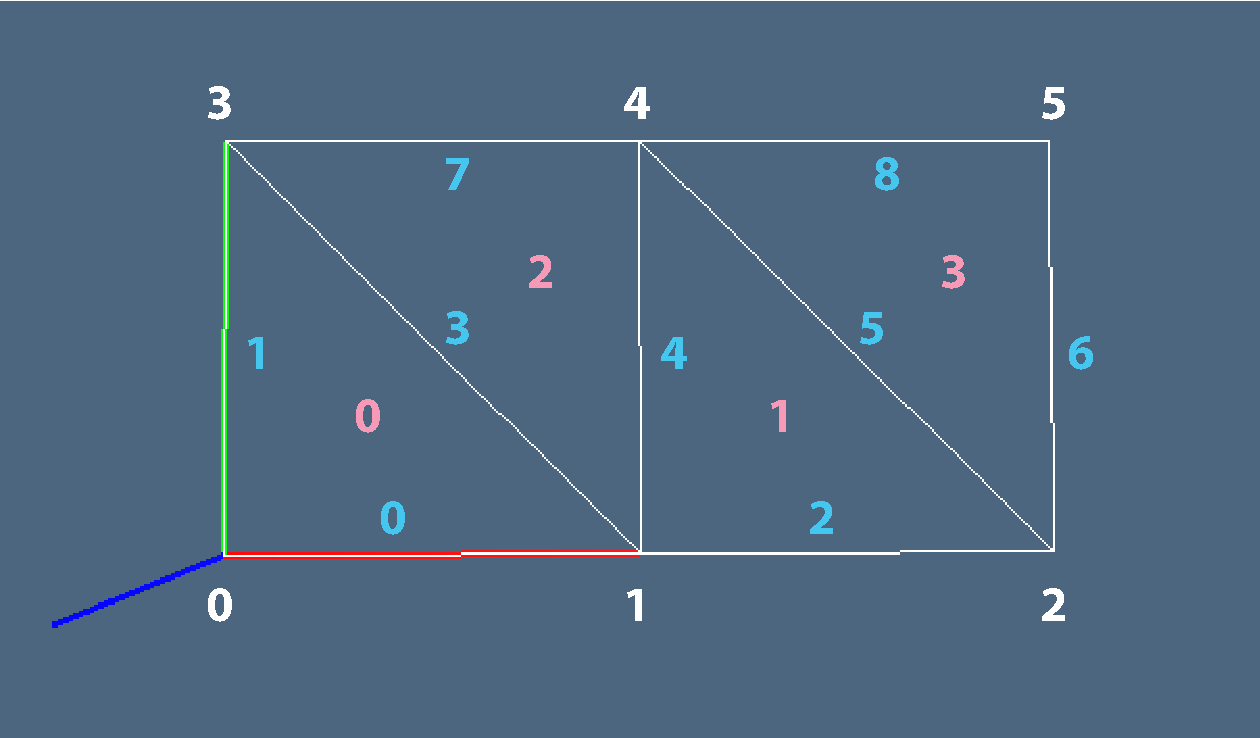
\includegraphics[width=0.6\linewidth]{images/2complex} 
   \caption{example caption}
   \label{fig:2complex}
\end{figure}

\paragraph{Matrix elements filtering}

Some filtering operations on matrix elements are needed in the implementation of various topological operators. Some of such filtering operations are given below.

%-------------------------------------------------------------------------------
\begin{flushleft} \small \label{scrap14}
\protect\makebox[0ex][r]{\NWtarget{nuweb8}{\rule{0ex}{0ex}}\hspace{1em}}$\langle\,$Matrix filtering to produce the boundary matrix\nobreak\ {\footnotesize 8}$\,\rangle\equiv$
\vspace{-1ex}
\begin{list}{}{} \item
\mbox{}\verb@def csrBoundaryFilter(CSRm, facetLengths):@\\
\mbox{}\verb@   maxs = [max(CSRm[k].data) for k in range(CSRm.shape[0])]@\\
\mbox{}\verb@   inputShape = CSRm.shape@\\
\mbox{}\verb@   coo = CSRm.tocoo()@\\
\mbox{}\verb@   for k in range(len(coo.data)):@\\
\mbox{}\verb@      if coo.data[k]==maxs[coo.row[k]]: coo.data[k] = 1@\\
\mbox{}\verb@      else: coo.data[k] = 0@\\
\mbox{}\verb@   mtx = coo_matrix((coo.data, (coo.row, coo.col)), shape=inputShape)@\\
\mbox{}\verb@   out = mtx.tocsr()@\\
\mbox{}\verb@   return out@\\
\mbox{}\verb@@{\NWsep}
\end{list}
\vspace{-1ex}
\footnotesize\addtolength{\baselineskip}{-1ex}
\begin{list}{}{\setlength{\itemsep}{-\parsep}\setlength{\itemindent}{-\leftmargin}}
\item \NWtxtMacroRefIn\ \NWlink{nuweb34b}{34b}.
\end{list}
\end{flushleft}
%-------------------------------------------------------------------------------
%-------------------------------------------------------------------------------
\begin{flushleft} \small \label{scrap15}
\protect\makebox[0ex][r]{\NWtarget{nuweb9a}{\rule{0ex}{0ex}}\hspace{1em}}$\langle\,$Test example of Matrix filtering to produce the boundary matrix\nobreak\ {\footnotesize 9a}$\,\rangle\equiv$
\vspace{-1ex}
\begin{list}{}{} \item
\mbox{}\verb@print "\n>>> csrBoundaryFilter"@\\
\mbox{}\verb@csrEF = matrixProduct(csrFV, csrTranspose(csrEV)).T@\\
\mbox{}\verb@facetLengths = [csrCell.getnnz() for csrCell in csrEV]@\\
\mbox{}\verb@CSRm = csrBoundaryFilter(csrEF, facetLengths).T@\\
\mbox{}\verb@print "\ncsrMaxFilter(csrFE) =\n", csr2DenseMatrix(CSRm)@\\
\mbox{}\verb@@{\NWsep}
\end{list}
\vspace{-1ex}
\footnotesize\addtolength{\baselineskip}{-1ex}
\begin{list}{}{\setlength{\itemsep}{-\parsep}\setlength{\itemindent}{-\leftmargin}}
\item \NWtxtMacroRefIn\ \NWlink{nuweb35a}{35a}.
\end{list}
\end{flushleft}
%-------------------------------------------------------------------------------
%-------------------------------------------------------------------------------
\begin{flushleft} \small \label{scrap16}
\protect\makebox[0ex][r]{\NWtarget{nuweb9b}{\rule{0ex}{0ex}}\hspace{1em}}$\langle\,$Matrix filtering via a generic predicate\nobreak\ {\footnotesize 9b}$\,\rangle\equiv$
\vspace{-1ex}
\begin{list}{}{} \item
\mbox{}\verb@def csrPredFilter(CSRm, pred):@\\
\mbox{}\verb@   # can be done in parallel (by rows)@\\
\mbox{}\verb@   coo = CSRm.tocoo()@\\
\mbox{}\verb@   triples = [[row,col,val] for row,col,val @\\
\mbox{}\verb@            in zip(coo.row,coo.col,coo.data) if pred(val)]@\\
\mbox{}\verb@   i, j, data = TRANS(triples)@\\
\mbox{}\verb@   CSRm = scipy.sparse.coo_matrix((data,(i,j)),CSRm.shape).tocsr()@\\
\mbox{}\verb@   return CSRm@\\
\mbox{}\verb@@{\NWsep}
\end{list}
\vspace{-1ex}
\footnotesize\addtolength{\baselineskip}{-1ex}
\begin{list}{}{\setlength{\itemsep}{-\parsep}\setlength{\itemindent}{-\leftmargin}}
\item \NWtxtMacroRefIn\ \NWlink{nuweb34b}{34b}.
\end{list}
\end{flushleft}
%-------------------------------------------------------------------------------
%-------------------------------------------------------------------------------
\begin{flushleft} \small \label{scrap17}
\protect\makebox[0ex][r]{\NWtarget{nuweb9c}{\rule{0ex}{0ex}}\hspace{1em}}$\langle\,$Test example of Matrix filtering via a generic predicate\nobreak\ {\footnotesize 9c}$\,\rangle\equiv$
\vspace{-1ex}
\begin{list}{}{} \item
\mbox{}\verb@print "\n>>> csrPredFilter"@\\
\mbox{}\verb@CSRm = csrPredFilter(matrixProduct(csrFV, csrTranspose(csrEV)).T, GE(2)).T@\\
\mbox{}\verb@print "\nccsrPredFilter(csrFE) =\n", csr2DenseMatrix(CSRm)@\\
\mbox{}\verb@@{\NWsep}
\end{list}
\vspace{-1ex}
\footnotesize\addtolength{\baselineskip}{-1ex}
\begin{list}{}{\setlength{\itemsep}{-\parsep}\setlength{\itemindent}{-\leftmargin}}
\item \NWtxtMacroRefIn\ \NWlink{nuweb35a}{35a}.
\end{list}
\end{flushleft}
%-------------------------------------------------------------------------------



\paragraph{Relational inversion (characteristic matrix transposition)}

The operation could be executed by simple matrix transposition of the CSR (Compressed Sparse Row) representation of the sparse characteristic matrix $M_d \equiv \texttt{CV}$.
A simple relational inversion using Python lists is given here. The \texttt{invertRelation} function 
is given here, linear in the size of the \texttt{CV} list, where the complexity of each cell is constant and 
small in most cases.

%-------------------------------------------------------------------------------
\begin{flushleft} \small \label{scrap18}
\protect\makebox[0ex][r]{\NWtarget{nuweb9d}{\rule{0ex}{0ex}}\hspace{1em}}$\langle\,$Characteristic matrix transposition\nobreak\ {\footnotesize 9d}$\,\rangle\equiv$
\vspace{-1ex}
\begin{list}{}{} \item
\mbox{}\verb@""" Characteristic matrix transposition """@\\
\mbox{}\verb@def invertRelation(CV):    @\\
\mbox{}\verb@    def myMax(List):@\\
\mbox{}\verb@        if List==[]:  return -1@\\
\mbox{}\verb@        else:  return max(List)@\\
\mbox{}\verb@            @\\
\mbox{}\verb@    columnNumber = max(AA(myMax)(CV))+1@\\
\mbox{}\verb@    VC = [[] for k in range(columnNumber)]@\\
\mbox{}\verb@    for k,cell in enumerate(CV):@\\
\mbox{}\verb@        for v in cell: VC[v] += [k]@\\
\mbox{}\verb@    return VC@\\
\mbox{}\verb@@{\NWsep}
\end{list}
\vspace{-1ex}
\footnotesize\addtolength{\baselineskip}{-1ex}
\begin{list}{}{\setlength{\itemsep}{-\parsep}\setlength{\itemindent}{-\leftmargin}}
\item \NWtxtMacroRefIn\ \NWlink{nuweb34b}{34b}.
\end{list}
\end{flushleft}
%-------------------------------------------------------------------------------


\subsection{Computation of lower-dimensional skeletons}

In most cases, in particular when the cellular complex is made by convex cells, the only cells of maximal dimension must be entered to gain a complete knowledge of the whole complex.
Here we show how to compute the $(d-1)$-skeleton of a complex starting from its $d$-dimensional skeleton.

\paragraph{Extraction of facets of a cell complex} 

The following \texttt{larFacets} function returns the LAR model \texttt{V,cellFacets} starting from the input \texttt{model} parameter. Two optional parameters define the (intrinsic) dimension of the input cells, with default value equal to three, and the eventual presence of a \texttt{emptyCellNumber} of empty cells. Their number default to zero when the complex is closed, for example in the case it provides the $d$-boundary of a $(d+1)$-complex. If empty cells are present, their subset must be located at the end of the \texttt{cell} list.

%-------------------------------------------------------------------------------
\begin{flushleft} \small \label{scrap19}
\protect\makebox[0ex][r]{\NWtarget{nuweb10}{\rule{0ex}{0ex}}\hspace{1em}}$\langle\,$Extraction of facets of a cell complex\nobreak\ {\footnotesize 10}$\,\rangle\equiv$
\vspace{-1ex}
\begin{list}{}{} \item
\mbox{}\verb@def setup(model,dim):@\\
\mbox{}\verb@   V, cells = model@\\
\mbox{}\verb@   csr = csrCreate(cells)@\\
\mbox{}\verb@   csrAdjSquareMat = larCellAdjacencies(csr)@\\
\mbox{}\verb@   csrAdjSquareMat = csrPredFilter(csrAdjSquareMat, GE(dim)) # ? HOWTODO ?@\\
\mbox{}\verb@   return V,cells,csr,csrAdjSquareMat@\\
\mbox{}\verb@@\\
\mbox{}\verb@def larFacets(model, dim=3, emptyCellNumber=0):@\\
\mbox{}\verb@   """ Estraction of (d-1)-cellFacets from "model" := (V,d-cells)@\\
\mbox{}\verb@      Return (V, (d-1)-cellFacets)@\\
\mbox{}\verb@      """@\\
\mbox{}\verb@   V,cells,csr,csrAdjSquareMat = setup(model,dim)@\\
\mbox{}\verb@   solidCellNumber = len(cells) - emptyCellNumber@\\
\mbox{}\verb@   cellFacets = []@\\
\mbox{}\verb@   # for each input cell i@\\
\mbox{}\verb@   for i in range(len(cells)):@\\
\mbox{}\verb@      adjCells = csrAdjSquareMat[i].tocoo()@\\
\mbox{}\verb@      cell1 = csr[i].tocoo().col@\\
\mbox{}\verb@      pairs = zip(adjCells.col,adjCells.data)@\\
\mbox{}\verb@      for j,v in pairs:@\\
\mbox{}\verb@         if (i<j) and (i<solidCellNumber):@\\
\mbox{}\verb@            cell2 = csr[j].tocoo().col@\\
\mbox{}\verb@            cell = list(set(cell1).intersection(cell2))@\\
\mbox{}\verb@            cellFacets.append(sorted(cell))@\\
\mbox{}\verb@   # sort and remove duplicates@\\
\mbox{}\verb@   cellFacets = sorted(AA(list)(set(AA(tuple)(cellFacets))))@\\
\mbox{}\verb@   return V,cellFacets@\\
\mbox{}\verb@@{\NWsep}
\end{list}
\vspace{-1ex}
\footnotesize\addtolength{\baselineskip}{-1ex}
\begin{list}{}{\setlength{\itemsep}{-\parsep}\setlength{\itemindent}{-\leftmargin}}
\item \NWtxtMacroRefIn\ \NWlink{nuweb34b}{34b}.
\end{list}
\end{flushleft}
%-------------------------------------------------------------------------------



%-------------------------------------------------------------------------------
\begin{flushleft} \small \label{scrap20}
\protect\makebox[0ex][r]{\NWtarget{nuweb11a}{\rule{0ex}{0ex}}\hspace{1em}}$\langle\,$Computation of cell adjacencies\nobreak\ {\footnotesize 11a}$\,\rangle\equiv$
\vspace{-1ex}
\begin{list}{}{} \item
\mbox{}\verb@def larCellAdjacencies(CSRm):@\\
\mbox{}\verb@   CSRm = matrixProduct(CSRm,csrTranspose(CSRm))@\\
\mbox{}\verb@   return CSRm@\\
\mbox{}\verb@@{\NWsep}
\end{list}
\vspace{-1ex}
\footnotesize\addtolength{\baselineskip}{-1ex}
\begin{list}{}{\setlength{\itemsep}{-\parsep}\setlength{\itemindent}{-\leftmargin}}
\item \NWtxtMacroRefIn\ \NWlink{nuweb34b}{34b}.
\end{list}
\end{flushleft}
%-------------------------------------------------------------------------------

\paragraph{Examples}
Two simple complexes are defined below by providing the pair \texttt{V,FV}.
In both cases the \texttt{EV} relation is computed via the \texttt{larFacets} function.
%-------------------------------------------------------------------------------
\begin{flushleft} \small \label{scrap21}
\protect\makebox[0ex][r]{\NWtarget{nuweb11b}{\rule{0ex}{0ex}}\hspace{1em}}$\langle\,$Test examples of Extraction of facets of a cell complex\nobreak\ {\footnotesize 11b}$\,\rangle\equiv$
\vspace{-1ex}
\begin{list}{}{} \item
\mbox{}\verb@""" A first (simplicial) example """@\\
\mbox{}\verb@V = [[0.,0.],[3.,0.],[0.,3.],[3.,3.],[1.,2.],[2.,2.],[1.,1.],[2.,1.]]@\\
\mbox{}\verb@FV = [[0,1,3],[1,2,4],[2,4,5],[3,4,6],[4,6,7],[5,7,8], # full@\\
\mbox{}\verb@   [1,3,4],[4,5,7], # empty@\\
\mbox{}\verb@   [0,1,2],[6,7,8],[0,3,6],[2,5,8]] # exterior     @\\
\mbox{}\verb@_,EV = larFacets((V,FV),dim=2)@\\
\mbox{}\verb@print "\nEV =",EV@\\
\mbox{}\verb@VIEW(EXPLODE(1.5,1.5,1.5)(MKPOLS((V,EV))))@\\
\mbox{}\verb@@\\
\mbox{}\verb@""" Another (cuboidal) example """@\\
\mbox{}\verb@FV = [[0,1,6,7],[0,2,4,6],[4,5,6,7],[1,3,5,7],[2,3,4,5],[0,1,2,3]]@\\
\mbox{}\verb@_,EV = larFacets((V,FV),dim=2)@\\
\mbox{}\verb@print "\nEV =",EV@\\
\mbox{}\verb@VV = AA(LIST)(range(len(V)))@\\
\mbox{}\verb@VIEW(EXPLODE(1.5,1.5,1.5)(MKPOLS((V,EV))))@\\
\mbox{}\verb@@{\NWsep}
\end{list}
\vspace{-1ex}
\footnotesize\addtolength{\baselineskip}{-1ex}
\begin{list}{}{\setlength{\itemsep}{-\parsep}\setlength{\itemindent}{-\leftmargin}}
\item \NWtxtMacroRefIn\ \NWlink{nuweb35a}{35a}.
\end{list}
\end{flushleft}
%-------------------------------------------------------------------------------

\paragraph{Visualization of cell numbers}
The adjacentcy matrices between 2-cells and 1-cells are printed here. Finally, the complex is displayed by numbering with different colours and sizes (depending on the rank) the complex cells.
%-------------------------------------------------------------------------------
\begin{flushleft} \small \label{scrap22}
\protect\makebox[0ex][r]{\NWtarget{nuweb11c}{\rule{0ex}{0ex}}\hspace{1em}}$\langle\,$Test examples of Computation of cell adjacencies\nobreak\ {\footnotesize 11c}$\,\rangle\equiv$
\vspace{-1ex}
\begin{list}{}{} \item
\mbox{}\verb@@\\
\mbox{}\verb@print "\n>>> larCellAdjacencies"@\\
\mbox{}\verb@adj_2_cells = larCellAdjacencies(csrCreate(FV))@\\
\mbox{}\verb@print "\nadj_2_cells =\n", csr2DenseMatrix(adj_2_cells)@\\
\mbox{}\verb@adj_1_cells = larCellAdjacencies(csrCreate(EV))@\\
\mbox{}\verb@print "\nadj_1_cells =\n", csr2DenseMatrix(adj_1_cells)@\\
\mbox{}\verb@@\\
\mbox{}\verb@submodel = mkSignedEdges((V,EV))@\\
\mbox{}\verb@VIEW(submodel)@\\
\mbox{}\verb@VIEW(larModelNumbering(scalx=1,scaly=1,scalz=1)(V,[VV,EV,FV],submodel,2))@\\
\mbox{}\verb@@{\NWsep}
\end{list}
\vspace{-1ex}
\footnotesize\addtolength{\baselineskip}{-1ex}
\begin{list}{}{\setlength{\itemsep}{-\parsep}\setlength{\itemindent}{-\leftmargin}}
\item \NWtxtMacroRefIn\ \NWlink{nuweb35a}{35a}.
\end{list}
\end{flushleft}
%-------------------------------------------------------------------------------


\section{Topological operations}

In this section we provide the matrix representation of operators to compute the more important and useful topological operations on cellular complexes, and/or the indexed relations they return. We start the section by giving a graphical tool used to test the developed software, concerning the graphical writing of the full set of indices of the cells of every dimension in a 3D cuboidal complex.  

\subsection{Visualization of cellular complexes}

It is often necessary to have a visual picture of the generated structures and computations.
This section provides some quite versatile visualisation tools of both the cells and/or their integer indices.

\paragraph{Visualization of cell indices}
As already outlined, the \texttt{modelIndexing} function return the \emph{hpc} value assembling both the 1-skeletons of the cells of every dimensions, and the graphical output of their indices, located on the centroid of each cell, and displayed using colors and sizes depending on the \emph{rank} of the cell.

%-------------------------------------------------------------------------------
\begin{flushleft} \small \label{scrap23}
\protect\makebox[0ex][r]{\NWtarget{nuweb12}{\rule{0ex}{0ex}}\hspace{1em}}$\langle\,$Visualization of cell indices\nobreak\ {\footnotesize 12}$\,\rangle\equiv$
\vspace{-1ex}
\begin{list}{}{} \item
\mbox{}\verb@""" Visualization of cell indices """@\\
\mbox{}\verb@from larlib import *@\\
\mbox{}\verb@@\\
\mbox{}\verb@def modelIndexing(shape):@\\
\mbox{}\verb@   V, bases = larCuboids(shape,True)@\\
\mbox{}\verb@   # bases = [[cell for cell in cellComplex if len(cell)==2**k] for k in range(4)]@\\
\mbox{}\verb@   color = [ORANGE,CYAN,GREEN,WHITE]@\\
\mbox{}\verb@   nums = AA(range)(AA(len)(bases))@\\
\mbox{}\verb@   hpcs = []@\\
\mbox{}\verb@   for k in range(4):@\\
\mbox{}\verb@      hpcs += [SKEL_1(STRUCT(MKPOLS((V,bases[k]))))]@\\
\mbox{}\verb@      hpcs += [cellNumbering((V,bases[k]),hpcs[2*k])(nums[k],color[k],0.3+0.2*k)]@\\
\mbox{}\verb@   return STRUCT(hpcs)@\\
\mbox{}\verb@@{\NWsep}
\end{list}
\vspace{-1ex}
\footnotesize\addtolength{\baselineskip}{-1ex}
\begin{list}{}{\setlength{\itemsep}{-\parsep}\setlength{\itemindent}{-\leftmargin}}
\item \NWtxtMacroDefBy\ \NWlink{nuweb12}{12}\NWlink{nuweb13a}{, 13a}.
\item \NWtxtMacroRefIn\ \NWlink{nuweb34b}{34b}.
\end{list}
\end{flushleft}
%-------------------------------------------------------------------------------


%-------------------------------------------------------------------------------
\begin{flushleft} \small \label{scrap24}
\protect\makebox[0ex][r]{\NWtarget{nuweb13a}{\rule{0ex}{0ex}}\hspace{1em}}$\langle\,$Visualization of cell indices\nobreak\ {\footnotesize 13a}$\,\rangle\equiv$
\vspace{-1ex}
\begin{list}{}{} \item
\mbox{}\verb@""" Numbered visualization of a LAR model """@\\
\mbox{}\verb@def larModelNumbering(scalx=1,scaly=1,scalz=1):@\\
\mbox{}\verb@   def  larModelNumbering0(V,bases,submodel,numberScaling=1):@\\
\mbox{}\verb@      color = [ORANGE,CYAN,GREEN,WHITE]@\\
\mbox{}\verb@      nums = AA(range)(AA(len)(bases))@\\
\mbox{}\verb@      hpcs = [submodel]@\\
\mbox{}\verb@      for k in range(len(bases)):@\\
\mbox{}\verb@         hpcs += [cellNumbering((V,bases[k]),submodel)@\\
\mbox{}\verb@                  (nums[k],color[k],(0.5+0.1*k)*numberScaling)]@\\
\mbox{}\verb@      return STRUCT(hpcs)@\\
\mbox{}\verb@      #return EXPLODE(scalx,scaly,scalz)(hpcs)@\\
\mbox{}\verb@   return larModelNumbering0@\\
\mbox{}\verb@@{\NWsep}
\end{list}
\vspace{-1ex}
\footnotesize\addtolength{\baselineskip}{-1ex}
\begin{list}{}{\setlength{\itemsep}{-\parsep}\setlength{\itemindent}{-\leftmargin}}
\item \NWtxtMacroDefBy\ \NWlink{nuweb12}{12}\NWlink{nuweb13a}{, 13a}.
\item \NWtxtMacroRefIn\ \NWlink{nuweb34b}{34b}.
\end{list}
\end{flushleft}
%-------------------------------------------------------------------------------



\paragraph{Drawing of oriented edges}
The following function return the \texttt{hpc} of the drawing with arrows of the oriented 1-cells of a 2D cellular complex. Of course, each edge orientation is from second to first vertex, independently from the vertex indices. Therefore, the edge orientation can be reversed by swapping the vertex indices in the 1-cell definition. 
%-------------------------------------------------------------------------------
\begin{flushleft} \small \label{scrap25}
\protect\makebox[0ex][r]{\NWtarget{nuweb13b}{\rule{0ex}{0ex}}\hspace{1em}}$\langle\,$Drawing of oriented edges\nobreak\ {\footnotesize 13b}$\,\rangle\equiv$
\vspace{-1ex}
\begin{list}{}{} \item
\mbox{}\verb@""" Drawing of oriented edges (2D) """@\\
\mbox{}\verb@def mkSignedEdges (model,scalingFactor=1):@\\
\mbox{}\verb@   V,EV = model@\\
\mbox{}\verb@   assert len(V[0])==2@\\
\mbox{}\verb@   hpcs = []@\\
\mbox{}\verb@   times = C(SCALARVECTPROD)@\\
\mbox{}\verb@   frac = 0.06*scalingFactor@\\
\mbox{}\verb@   for e0,e1 in EV:@\\
\mbox{}\verb@      v0,v1 = V[e0], V[e1]@\\
\mbox{}\verb@      vx,vy = DIFF([ v1, v0 ])@\\
\mbox{}\verb@      nx,ny = [-vy, vx]@\\
\mbox{}\verb@      v2 = SUM([ v0, times(0.66)([vx,vy]) ])@\\
\mbox{}\verb@      v3 = SUM([ v0, times(0.6-frac)([vx,vy]), times(frac)([nx,ny]) ])@\\
\mbox{}\verb@      v4 = SUM([ v0, times(0.6-frac)([vx,vy]), times(-frac)([nx,ny]) ])@\\
\mbox{}\verb@      verts,cells = [v0,v1,v2,v3,v4],[[1,2],[3,4],[3,5]]@\\
\mbox{}\verb@      hpcs += [MKPOL([verts,cells,None])]@\\
\mbox{}\verb@   hpc = STRUCT(hpcs)@\\
\mbox{}\verb@   return hpc@\\
\mbox{}\verb@@{\NWsep}
\end{list}
\vspace{-1ex}
\footnotesize\addtolength{\baselineskip}{-1ex}
\begin{list}{}{\setlength{\itemsep}{-\parsep}\setlength{\itemindent}{-\leftmargin}}
\item \NWtxtMacroRefIn\ \NWlink{nuweb34b}{34b}.
\end{list}
\end{flushleft}
%-------------------------------------------------------------------------------

\paragraph{Example of oriented edge drawing}
An example of drawing of oriented edges is given in \texttt{test/py/larcc/test11.py} file, and in Figure~\ref{numberedcomplex}, showing both the numbering of the cells and the arrows indicating the edge orientation is illustrated in Figure~\ref{numberedcomplex}, where also the oriented boundary is shown.

\begin{figure}[htbp] %  figure placement: here, top, bottom, or page
   \centering
   \includegraphics[width=0.9\linewidth]{images/numberedcomplex} 
   
   \includegraphics[width=0.9\linewidth]{images/numberedcomplex1} 
   \caption{Example of numbered polytopal complex, including edge orientations, and its oriented boundary.}
   \label{numberedcomplex}
\end{figure}

%-------------------------------------------------------------------------------
\begin{flushleft} \small \label{scrap26}
\protect\makebox[0ex][r]{\NWtarget{nuweb14a}{\rule{0ex}{0ex}}\hspace{1em}}\verb@"test/py/larcc/test11.py"@\nobreak\ {\footnotesize 14a }$\equiv$
\vspace{-1ex}
\begin{list}{}{} \item
\mbox{}\verb@@\\
\mbox{}\verb@@\hbox{$\langle\,$Example of oriented edge drawing\nobreak\ {\footnotesize \NWlink{nuweb14b}{14b}}$\,\rangle$}\verb@@\\
\mbox{}\verb@@{\NWsep}
\end{list}
\vspace{-2ex}
\end{flushleft}
%-------------------------------------------------------------------------------

%-------------------------------------------------------------------------------
\begin{flushleft} \small \label{scrap27}
\protect\makebox[0ex][r]{\NWtarget{nuweb14b}{\rule{0ex}{0ex}}\hspace{1em}}$\langle\,$Example of oriented edge drawing\nobreak\ {\footnotesize 14b}$\,\rangle\equiv$
\vspace{-1ex}
\begin{list}{}{} \item
\mbox{}\verb@""" Example of oriented edge drawing """@\\
\mbox{}\verb@from larlib import *@\\
\mbox{}\verb@@\\
\mbox{}\verb@V = [[9,0],[13,2],[15,4],[17,8],[14,9],[13,10],[11,11],[9,10],[7,9],[5,9],[3,@\\
\mbox{}\verb@8],[0,6],[2,3],[2,1],[5,0],[7,1],[4,2],[12,10],[6,3],[8,3],[3,5],[5,5],[7,6],@\\
\mbox{}\verb@[8,5],[10,5],[11,4],[10,2],[13,4],[14,6],[13,7],[11,9],[9,7],[7,7],[4,7],[2,@\\
\mbox{}\verb@6],[12,7],[12,5]]@\\
\mbox{}\verb@@\\
\mbox{}\verb@FV = [[0,1,26],[5,6,17],[6,7,17,30],[7,30,31],[7,8,31,32],[24,30,31,35],[3,4,@\\
\mbox{}\verb@28],[4,5,17,29,30,35],[4,28,29],[28,29,35,36],[8,9,32,33],[9,10,33],[11,10,@\\
\mbox{}\verb@33,34],[11,20,34],[20,33,34],[20,21,32,33],[18,21,22],[21,22,32],[22,23,31,@\\
\mbox{}\verb@32],[23,24,31],[11,12,20],[12,16,18,20,21],[18,22,23],[18,19,23],[19,23,24],@\\
\mbox{}\verb@[15,19,24,26],[0,15,26],[24,25,26],[24,25,35,36],[2,3,28],[1,2,27,28],[12,13,@\\
\mbox{}\verb@16],[13,14,16],[14,15,16,18,19],[1,25,26,27],[25,27,36],[36,27,28]]@\\
\mbox{}\verb@@\\
\mbox{}\verb@VIEW(EXPLODE(1.2,1.2,1)(MKPOLS((V,FV))))@\\
\mbox{}\verb@VV = AA(LIST)(range(len(V)))@\\
\mbox{}\verb@_,EV = larFacets((V,FV+[range(16)]),dim=2,emptyCellNumber=1)@\\
\mbox{}\verb@@\\
\mbox{}\verb@submodel = mkSignedEdges((V,EV))@\\
\mbox{}\verb@VIEW(submodel)@\\
\mbox{}\verb@VIEW(larModelNumbering(scalx=1,scaly=1,scalz=1)(V,[VV,EV,FV],submodel,2))@\\
\mbox{}\verb@@\\
\mbox{}\verb@orientedBoundary = signedCellularBoundaryCells(V,[VV,EV,FV])@\\
\mbox{}\verb@cells = [EV[e] if sign==1 else REVERSE(EV[e]) for (sign,e) in zip(*orientedBoundary)]@\\
\mbox{}\verb@submodel = mkSignedEdges((V,cells))@\\
\mbox{}\verb@VIEW(submodel)@\\
\mbox{}\verb@@{\NWsep}
\end{list}
\vspace{-1ex}
\footnotesize\addtolength{\baselineskip}{-1ex}
\begin{list}{}{\setlength{\itemsep}{-\parsep}\setlength{\itemindent}{-\leftmargin}}
\item \NWtxtMacroRefIn\ \NWlink{nuweb14a}{14a}\NWlink{nuweb16}{, 16}.
\end{list}
\end{flushleft}
%-------------------------------------------------------------------------------


\paragraph{Extracting the boundary of whichever chain}

The boundary of whichever chain, here defined as the list of indices of its cells, then transformed to its coordinate representation (column vector in the given basis), is explicitly computed by matrix product times the matrix of the boundary operator in the given basis, transformed back in its BRC representation, and displayed as  LAR model.
%-------------------------------------------------------------------------------
\begin{flushleft} \small \label{scrap28}
\protect\makebox[0ex][r]{\NWtarget{nuweb16}{\rule{0ex}{0ex}}\hspace{1em}}\verb@"test/py/larcc/test19.py"@\nobreak\ {\footnotesize 16 }$\equiv$
\vspace{-1ex}
\begin{list}{}{} \item
\mbox{}\verb@""" Example of oriented edge drawing """@\\
\mbox{}\verb@@\\
\mbox{}\verb@@\hbox{$\langle\,$Example of oriented edge drawing\nobreak\ {\footnotesize \NWlink{nuweb14b}{14b}}$\,\rangle$}\verb@@\\
\mbox{}\verb@@\\
\mbox{}\verb@C2 = csr_matrix((len(FV),1))@\\
\mbox{}\verb@for i in [1,2, 12,13,14,15, 22,23, 29,30,31]: C2[i,0] = 1@\\
\mbox{}\verb@BD = boundary(FV,EV)@\\
\mbox{}\verb@C1 = BD * C2@\\
\mbox{}\verb@C_1 = [i for i in range(len(EV)) if ABS(C1[i,0]) == 1 ]@\\
\mbox{}\verb@C_2 = [i for i in range(len(FV)) if C2[i,0] == 1 ]@\\
\mbox{}\verb@@\\
\mbox{}\verb@VIEW(EXPLODE(1.2,1.2,1)(MKPOLS((V,[EV[k] for k in C_1] + [FV[k] for k in C_2]))))@\\
\mbox{}\verb@@{\NWsep}
\end{list}
\vspace{-2ex}
\end{flushleft}
%-------------------------------------------------------------------------------




\subsection{Incidence and adjacency operators}

Let us start by computing the more interesting subset of the binary relationships between the 4 decompositive and/or boundary entities of 3D cellular models.  Therefore, in this case we denote with \texttt{C}, \texttt{F}, \texttt{E}, and \texttt{V}, the 3-cells and their faces, edges and vertices, respectively.
The input is the full-fledged LAR representation provided by 
\begin{align}
\texttt{CV} := \texttt{CSR}(M_3) \\
\texttt{FV} := \texttt{CSR}(M_2) \\
\texttt{EV} := \texttt{CSR}(M_1) \\
\texttt{VV} := \texttt{CSR}(M_0) 
\end{align}

Of course, $\texttt{CSR}(M_0)$ coincides with the identity matrix of dimension $|V|$ and can by excluded by further considerations.
Some binary incidence and adjacency relations we are going to compute are:
\begin{align}
\texttt{CF} := \texttt{CV} \times \texttt{FV}^t = \texttt{CSR}(M_3)\times\texttt{CSR}(M_2)^t \\
\texttt{CE} := \texttt{CV} \times \texttt{EV}^t = \texttt{CSR}(M_3)\times\texttt{CSR}(M_1)^t \\
\texttt{FE} := \texttt{FV} \times \texttt{EV}^t = \texttt{CSR}(M_2)\times\texttt{CSR}(M_1)^t 
\end{align}

The other possible operators follow from a similer computational pattern.

\paragraph{The programming pattern for incidence computation}

A high-level function \texttt{larIncidence} useful to compute the LAR representation of the incidence matrix (operator) and the incidence relations is given in the script below.

%-------------------------------------------------------------------------------
\begin{flushleft} \small \label{scrap29}
\protect\makebox[0ex][r]{\NWtarget{nuweb17a}{\rule{0ex}{0ex}}\hspace{1em}}$\langle\,$Some incidence operators\nobreak\ {\footnotesize 17a}$\,\rangle\equiv$
\vspace{-1ex}
\begin{list}{}{} \item
\mbox{}\verb@""" Some incidence operators """@\\
\mbox{}\verb@def larIncidence(cells,facets):@\\
\mbox{}\verb@   csrCellFacet = csrCellFaceIncidence(cells,facets)@\\
\mbox{}\verb@   cooCellFacet = csrCellFacet.tocoo()@\\
\mbox{}\verb@   larCellFacet = [[] for cell in range(len(cells))]@\\
\mbox{}\verb@   for i,j,val in zip(cooCellFacet.row,cooCellFacet.col,cooCellFacet.data):@\\
\mbox{}\verb@      if val == 1: larCellFacet[i] += [j]@\\
\mbox{}\verb@   return larCellFacet@\\
\mbox{}\verb@@\\
\mbox{}\verb@@\hbox{$\langle\,$Cell-Face incidence operator\nobreak\ {\footnotesize \NWlink{nuweb17b}{17b}}$\,\rangle$}\verb@@\\
\mbox{}\verb@@\hbox{$\langle\,$Cell-Edge incidence operator\nobreak\ {\footnotesize \NWlink{nuweb17c}{17c}}$\,\rangle$}\verb@@\\
\mbox{}\verb@@\hbox{$\langle\,$Face-Edge incidence operator\nobreak\ {\footnotesize \NWlink{nuweb18a}{18a}}$\,\rangle$}\verb@@\\
\mbox{}\verb@@{\NWsep}
\end{list}
\vspace{-1ex}
\footnotesize\addtolength{\baselineskip}{-1ex}
\begin{list}{}{\setlength{\itemsep}{-\parsep}\setlength{\itemindent}{-\leftmargin}}
\item \NWtxtMacroRefIn\ \NWlink{nuweb34b}{34b}.
\end{list}
\end{flushleft}
%-------------------------------------------------------------------------------


\paragraph{Cell-Face incidence}
The \texttt{csrCellFaceIncidence} and \texttt{larCellFace} functions are given below, and exported to the \texttt{larcc} module.
%-------------------------------------------------------------------------------
\begin{flushleft} \small \label{scrap30}
\protect\makebox[0ex][r]{\NWtarget{nuweb17b}{\rule{0ex}{0ex}}\hspace{1em}}$\langle\,$Cell-Face incidence operator\nobreak\ {\footnotesize 17b}$\,\rangle\equiv$
\vspace{-1ex}
\begin{list}{}{} \item
\mbox{}\verb@""" Cell-Face incidence operator """@\\
\mbox{}\verb@def csrCellFaceIncidence(CV,FV):@\\
\mbox{}\verb@   return boundary(FV,CV)@\\
\mbox{}\verb@@\\
\mbox{}\verb@def larCellFace(CV,FV):@\\
\mbox{}\verb@   return larIncidence(CV,FV)@\\
\mbox{}\verb@@{\NWsep}
\end{list}
\vspace{-1ex}
\footnotesize\addtolength{\baselineskip}{-1ex}
\begin{list}{}{\setlength{\itemsep}{-\parsep}\setlength{\itemindent}{-\leftmargin}}
\item \NWtxtMacroRefIn\ \NWlink{nuweb17a}{17a}.
\end{list}
\end{flushleft}
%-------------------------------------------------------------------------------

\paragraph{Cell-Edge incidence}
Analogously, the \texttt{csrCellEdgeIncidence} and \texttt{larCellFace} functions are given in the following script.

%-------------------------------------------------------------------------------
\begin{flushleft} \small \label{scrap31}
\protect\makebox[0ex][r]{\NWtarget{nuweb17c}{\rule{0ex}{0ex}}\hspace{1em}}$\langle\,$Cell-Edge incidence operator\nobreak\ {\footnotesize 17c}$\,\rangle\equiv$
\vspace{-1ex}
\begin{list}{}{} \item
\mbox{}\verb@""" Cell-Edge incidence operator """@\\
\mbox{}\verb@def csrCellEdgeIncidence(CV,EV):@\\
\mbox{}\verb@    return boundary(EV,CV)@\\
\mbox{}\verb@@\\
\mbox{}\verb@def larCellEdge(CV,EV):@\\
\mbox{}\verb@   return larIncidence(CV,EV)@\\
\mbox{}\verb@@{\NWsep}
\end{list}
\vspace{-1ex}
\footnotesize\addtolength{\baselineskip}{-1ex}
\begin{list}{}{\setlength{\itemsep}{-\parsep}\setlength{\itemindent}{-\leftmargin}}
\item \NWtxtMacroRefIn\ \NWlink{nuweb17a}{17a}.
\end{list}
\end{flushleft}
%-------------------------------------------------------------------------------

\paragraph{Face-Edge incidence}
Finally, the \texttt{csrCellEdgeIncidence} and \texttt{larCellFace} functions are provided below.

%-------------------------------------------------------------------------------
\begin{flushleft} \small \label{scrap32}
\protect\makebox[0ex][r]{\NWtarget{nuweb18a}{\rule{0ex}{0ex}}\hspace{1em}}$\langle\,$Face-Edge incidence operator\nobreak\ {\footnotesize 18a}$\,\rangle\equiv$
\vspace{-1ex}
\begin{list}{}{} \item
\mbox{}\verb@""" Face-Edge incidence operator """@\\
\mbox{}\verb@def csrFaceEdgeIncidence(FV,EV):@\\
\mbox{}\verb@   return boundary(EV,FV)@\\
\mbox{}\verb@@\\
\mbox{}\verb@def larFaceEdge(FV,EV):@\\
\mbox{}\verb@   return larIncidence(FV,EV)@\\
\mbox{}\verb@@{\NWsep}
\end{list}
\vspace{-1ex}
\footnotesize\addtolength{\baselineskip}{-1ex}
\begin{list}{}{\setlength{\itemsep}{-\parsep}\setlength{\itemindent}{-\leftmargin}}
\item \NWtxtMacroRefIn\ \NWlink{nuweb17a}{17a}.
\end{list}
\end{flushleft}
%-------------------------------------------------------------------------------


\paragraph{Example}
The example below concerns a 3D cuboidal grid, by computing a full LAR stack of bases
\texttt{CV, FV, EV, VV}, showing its fully numbered 3D model, and finally by computing
some more useful binary relationships (\texttt{CF, CE, FE}), needed for example to compute the signed matrices of boundary operators.

%-------------------------------------------------------------------------------
\begin{flushleft} \small \label{scrap33}
\protect\makebox[0ex][r]{\NWtarget{nuweb18b}{\rule{0ex}{0ex}}\hspace{1em}}\verb@"test/py/larcc/test10.py"@\nobreak\ {\footnotesize 18b }$\equiv$
\vspace{-1ex}
\begin{list}{}{} \item
\mbox{}\verb@""" A mesh model and various incidence operators """@\\
\mbox{}\verb@@\\
\mbox{}\verb@from larlib import *@\\
\mbox{}\verb@@\\
\mbox{}\verb@shape = [2,2,2]@\\
\mbox{}\verb@V,(VV,EV,FV,CV) = larCuboids(shape,True)@\\
\mbox{}\verb@VIEW(modelIndexing(shape))@\\
\mbox{}\verb@@\\
\mbox{}\verb@CF = larCellFace(CV,FV)@\\
\mbox{}\verb@CE = larCellFace(CV,EV)@\\
\mbox{}\verb@FE = larCellFace(FV,EV)@\\
\mbox{}\verb@@{\NWsep}
\end{list}
\vspace{-2ex}
\end{flushleft}
%-------------------------------------------------------------------------------

\subsubsection{Incidence chain}

Let denote with \texttt{CF}, \texttt{FE}, \texttt{EV} the three consecutive incidence relations between $k$-cells and $(k-1)$-cells ($3\leq k\leq 0$) in a 3-complex. In the general multidimensional case, let us call \texttt{CF}$_d$  the generic \emph{binary} incidence operator, between $d$-cells and $(d-1)$-facets, as:
\[
\texttt{CF}_d = M_{d-1} M_d^t, 
\]
with
\[
\texttt{CF}_d := \{a_{ij}\}, \qquad a_{ij} = 
\left\{
\begin{array}{cl}
1 & \mbox{if\ } M_{d-1}(i) M_d(j) = |f_j|  \\
0 & \mbox{otherwise}  \\  
\end{array}
\right.
\]

\paragraph{Incidence chain computation}
The function \texttt{incidenceChain}, given below, returns the full stack of \texttt{BRC} incidence matrices of a LAR representation for a cellular complex, starting from its list of bases, i.e.~from \texttt{[VV,EV,FV,CV,...]}. Notice that the function returns the inverse sequence 
\texttt{[EV,FE,CF,...]}, i.e., \texttt{CF}$_k$ ($1\leq k\leq d$).

%-------------------------------------------------------------------------------
\begin{flushleft} \small \label{scrap34}
\protect\makebox[0ex][r]{\NWtarget{nuweb19a}{\rule{0ex}{0ex}}\hspace{1em}}$\langle\,$Incidence chain computation\nobreak\ {\footnotesize 19a}$\,\rangle\equiv$
\vspace{-1ex}
\begin{list}{}{} \item
\mbox{}\verb@""" Incidence chain computation """@\\
\mbox{}\verb@def incidenceChain(bases):@\\
\mbox{}\verb@   #print "\n len(bases) = ",len(bases),"\n"@\\
\mbox{}\verb@   pairsOfBases = zip(bases[1:],bases[:-1])@\\
\mbox{}\verb@   relations = [larIncidence(cells,facets) @\\
\mbox{}\verb@               for cells,facets in pairsOfBases]@\\
\mbox{}\verb@   return REVERSE(relations)@\\
\mbox{}\verb@@{\NWsep}
\end{list}
\vspace{-1ex}
\footnotesize\addtolength{\baselineskip}{-1ex}
\begin{list}{}{\setlength{\itemsep}{-\parsep}\setlength{\itemindent}{-\leftmargin}}
\item \NWtxtMacroRefIn\ \NWlink{nuweb34b}{34b}.
\end{list}
\end{flushleft}
%-------------------------------------------------------------------------------

%-------------------------------------------------------------------------------
\begin{flushleft} \small \label{scrap35}
\protect\makebox[0ex][r]{\NWtarget{nuweb19b}{\rule{0ex}{0ex}}\hspace{1em}}\verb@"test/py/larcc/test13.py"@\nobreak\ {\footnotesize 19b }$\equiv$
\vspace{-1ex}
\begin{list}{}{} \item
\mbox{}\verb@""" Example of incidence chain computation """@\\
\mbox{}\verb@from larlib import *@\\
\mbox{}\verb@@\\
\mbox{}\verb@shape = (1,1,2) @\\
\mbox{}\verb@print "\n\nFor a better example provide a greater shape!"@\\
\mbox{}\verb@V,bases = larCuboids(shape,True)@\\
\mbox{}\verb@@\\
\mbox{}\verb@VV,EV,FV,CV = bases@\\
\mbox{}\verb@incidence = incidenceChain([VV,EV,FV,CV])@\\
\mbox{}\verb@relations = ["CF","FE","EV"]@\\
\mbox{}\verb@for k in range(3):@\\
\mbox{}\verb@   print "\n\n incidence", relations[k], "=\n", incidence[k],@\\
\mbox{}\verb@print "\n\n"@\\
\mbox{}\verb@@\\
\mbox{}\verb@submodel = SKEL_1(STRUCT(MKPOLS((V,EV))))@\\
\mbox{}\verb@VIEW(larModelNumbering(scalx=1,scaly=1,scalz=1)(V,[VV,EV,FV,CV],submodel,1))@\\
\mbox{}\verb@@{\NWsep}
\end{list}
\vspace{-2ex}
\end{flushleft}
%-------------------------------------------------------------------------------


\paragraph{Example of incidence chain computation}
When running the \texttt{test/py/larcc/test13.py} file one obtains the following printout. 
Notice that 
it provides the links between $d$-cell numerations and the numerations of their faces.
See Figure~\ref{incidenceChain} for this purpose.

\begin{figure}[htbp] %  figure placement: here, top, bottom, or page
   \centering
   \includegraphics[width=0.5\linewidth]{images/incidenceChain} 
   \caption{Che stack of incidence relations gives the common links between cell numerations.}
   \label{incidenceChain}
\end{figure}


%-------------------------------------------------------------------------------
\begin{flushleft} \small \label{scrap36}
\protect\makebox[0ex][r]{\NWtarget{nuweb19c}{\rule{0ex}{0ex}}\hspace{1em}}$\langle\,$Incidence chain for a 3D cuboidal complex\nobreak\ {\footnotesize 19c}$\,\rangle\equiv$
\vspace{-1ex}
\begin{list}{}{} \item
\mbox{}\verb@incidence CF = [[0,2,4,6,8,9],[1,3,5,7,9,10]]@\\
\mbox{}\verb@@\\
\mbox{}\verb@incidence FE = [[0,2,8,9],[1,3,9,10],[4,6,11,12],[5,7,12,13],[0,4,14,15],@\\
\mbox{}\verb@[1,5,15,16],[2,6,17,18],[3,7,18,19],[8,11,14,17],[9,12,15,18],[10,13,16,19]]@\\
\mbox{}\verb@@\\
\mbox{}\verb@incidence EV = [[0,1],[1,2],[3,4],[4,5],[6,7],[7,8],[9,10],[10,11],[0,3],@\\
\mbox{}\verb@[1,4],[2,5],[6,9],[7,10],[8,11],[0,6],[1,7],[2,8],[3,9],[4,10],[5,11]]@\\
\mbox{}\verb@@{\NWsep}
\end{list}
\vspace{-1ex}
\footnotesize\addtolength{\baselineskip}{-1ex}
\begin{list}{}{\setlength{\itemsep}{-\parsep}\setlength{\itemindent}{-\leftmargin}}
\item {\NWtxtMacroNoRef}.
\end{list}
\end{flushleft}
%-------------------------------------------------------------------------------



\subsection{Boundary and coboundary operators}

When computing the matrices of boundary and coboundary operators it may be useful to distinguish between simplicial complexes and general polytopal complexes, including  cuboidal ones. In the first cases all skeletons, and hence the other topological operators, may be computed using only combinatorial methods. In the second case some reference to their geometric embedding must be done, at least to compute the \emph{oriented} boundary and coboundary. Therefore we separate the two cases in the following sections.


\subsubsection{Non-oriented operators}

The \texttt{boundary} function below takes as parameters the \texttt{BRC} representations of $d$-cells and $(d-1)$-facets, and returns the \texttt{CSR} matrix of the boundary operator. Let us notice that such operator uses a mod 2 algebra, since it takes elements within the field $\Z_2=\{0,1\}$.

%-------------------------------------------------------------------------------
\begin{flushleft} \small \label{scrap37}
\protect\makebox[0ex][r]{\NWtarget{nuweb20}{\rule{0ex}{0ex}}\hspace{1em}}$\langle\,$Test examples of From cells and facets to boundary operator\nobreak\ {\footnotesize 20}$\,\rangle\equiv$
\vspace{-1ex}
\begin{list}{}{} \item
\mbox{}\verb@V = [[0.0,0.0,0.0],[1.0,0.0,0.0],[0.0,1.0,0.0],[1.0,1.0,0.0],@\\
\mbox{}\verb@      [0.0,0.0,1.0],[1.0,0.0,1.0],[0.0,1.0,1.0],[1.0,1.0,1.0]]@\\
\mbox{}\verb@CV = [[0,1,2,4],[1,2,4,5],[2,4,5,6],[1,2,3,5],[2,3,5,6],[3,5,6,7]]@\\
\mbox{}\verb@FV = [[0,1,2],[0,1,4],[0,2,4],[1,2,3],[1,2,4],[1,2,5],[1,3,5],[1,4,5],[2,3,5],@\\
\mbox{}\verb@     [2,3,6],[2,4,5],[2,4,6],[2,5,6],[3,5,6],[3,5,7],[3,6,7],[4,5,6],[5,6,7]]@\\
\mbox{}\verb@EV = [[0,1],[0,2],[0,4],[1,2],[1,3],[1,4],[1,5],[2,3],[2,4],[2,5],@\\
\mbox{}\verb@     [2,6],[3,5],[3,6],[3,7],[4,5],[4,6],[5,6],[5,7],[6,7]]@\\
\mbox{}\verb@VV = AA(LIST)(range(len(V)))@\\
\mbox{}\verb@@\\
\mbox{}\verb@print "\ncoboundary_2 =\n", csr2DenseMatrix(coboundary(CV,FV))@\\
\mbox{}\verb@print "\ncoboundary_1 =\n", csr2DenseMatrix(coboundary(FV,EV))@\\
\mbox{}\verb@print "\ncoboundary_0 =\n", csr2DenseMatrix(coboundary(EV,VV))@\\
\mbox{}\verb@@{\NWsep}
\end{list}
\vspace{-1ex}
\footnotesize\addtolength{\baselineskip}{-1ex}
\begin{list}{}{\setlength{\itemsep}{-\parsep}\setlength{\itemindent}{-\leftmargin}}
\item \NWtxtMacroRefIn\ \NWlink{nuweb35a}{35a}.
\end{list}
\end{flushleft}
%-------------------------------------------------------------------------------

In the script below it is necessary to guarantee that both \texttt{csrFV} and \texttt{csrCV} are created with the same number of column. The initial steps have this purpose.

%-------------------------------------------------------------------------------
\begin{flushleft} \small \label{scrap38}
\protect\makebox[0ex][r]{\NWtarget{nuweb21a}{\rule{0ex}{0ex}}\hspace{1em}}$\langle\,$From cells and facets to boundary operator\nobreak\ {\footnotesize 21a}$\,\rangle\equiv$
\vspace{-1ex}
\begin{list}{}{} \item
\mbox{}\verb@def boundary(cells,facets):@\\
\mbox{}\verb@   lenV = max(max(cells),max(facets))@\\
\mbox{}\verb@   csrCV = csrCreate(cells,lenV)@\\
\mbox{}\verb@   csrFV = csrCreate(facets,lenV)@\\
\mbox{}\verb@   csrFC = matrixProduct(csrFV, csrTranspose(csrCV))@\\
\mbox{}\verb@   facetLengths = [csrCell.getnnz() for csrCell in csrCV]@\\
\mbox{}\verb@   return csrBoundaryFilter(csrFC,facetLengths)@\\
\mbox{}\verb@@\\
\mbox{}\verb@def coboundary(cells,facets):@\\
\mbox{}\verb@   Boundary = boundary(cells,facets)@\\
\mbox{}\verb@   return csrTranspose(Boundary)@\\
\mbox{}\verb@@{\NWsep}
\end{list}
\vspace{-1ex}
\footnotesize\addtolength{\baselineskip}{-1ex}
\begin{list}{}{\setlength{\itemsep}{-\parsep}\setlength{\itemindent}{-\leftmargin}}
\item \NWtxtMacroRefIn\ \NWlink{nuweb34b}{34b}.
\end{list}
\end{flushleft}
%-------------------------------------------------------------------------------
%-------------------------------------------------------------------------------
\begin{flushleft} \small \label{scrap39}
\protect\makebox[0ex][r]{\NWtarget{nuweb21b}{\rule{0ex}{0ex}}\hspace{1em}}$\langle\,$From cells and facets to boundary cells\nobreak\ {\footnotesize 21b}$\,\rangle\equiv$
\vspace{-1ex}
\begin{list}{}{} \item
\mbox{}\verb@def totalChain(cells):@\\
\mbox{}\verb@   return csrCreate([[0] for cell in cells])  # ????  zero ??@\\
\mbox{}\verb@@\\
\mbox{}\verb@def boundaryCells(cells,facets):@\\
\mbox{}\verb@   csrBoundaryMat = boundary(cells,facets)@\\
\mbox{}\verb@   csrChain = totalChain(cells)@\\
\mbox{}\verb@   csrBoundaryChain = matrixProduct(csrBoundaryMat, csrChain)@\\
\mbox{}\verb@   for k,value in enumerate(csrBoundaryChain.data):@\\
\mbox{}\verb@      if value % 2 == 0: csrBoundaryChain.data[k] = 0@\\
\mbox{}\verb@   out = [k for k,val in enumerate(csrBoundaryChain.data.tolist()) if val == 1]@\\
\mbox{}\verb@   return out@\\
\mbox{}\verb@@{\NWsep}
\end{list}
\vspace{-1ex}
\footnotesize\addtolength{\baselineskip}{-1ex}
\begin{list}{}{\setlength{\itemsep}{-\parsep}\setlength{\itemindent}{-\leftmargin}}
\item \NWtxtMacroRefIn\ \NWlink{nuweb34b}{34b}.
\end{list}
\end{flushleft}
%-------------------------------------------------------------------------------
%-------------------------------------------------------------------------------
\begin{flushleft} \small \label{scrap40}
\protect\makebox[0ex][r]{\NWtarget{nuweb21c}{\rule{0ex}{0ex}}\hspace{1em}}$\langle\,$Test examples of From cells and facets to boundary cells\nobreak\ {\footnotesize 21c}$\,\rangle\equiv$
\vspace{-1ex}
\begin{list}{}{} \item
\mbox{}\verb@boundaryCells_2 = boundaryCells(CV,FV)@\\
\mbox{}\verb@boundaryCells_1 = boundaryCells([FV[k] for k in boundaryCells_2],EV)@\\
\mbox{}\verb@@\\
\mbox{}\verb@print "\nboundaryCells_2 =\n", boundaryCells_2@\\
\mbox{}\verb@print "\nboundaryCells_1 =\n", boundaryCells_1@\\
\mbox{}\verb@@\\
\mbox{}\verb@boundaryModel = (V,[FV[k] for k in boundaryCells_2])@\\
\mbox{}\verb@VIEW(EXPLODE(1.5,1.5,1.5)(MKPOLS(boundaryModel)))@\\
\mbox{}\verb@@{\NWsep}
\end{list}
\vspace{-1ex}
\footnotesize\addtolength{\baselineskip}{-1ex}
\begin{list}{}{\setlength{\itemsep}{-\parsep}\setlength{\itemindent}{-\leftmargin}}
\item \NWtxtMacroRefIn\ \NWlink{nuweb35a}{35a}.
\end{list}
\end{flushleft}
%-------------------------------------------------------------------------------



\subsubsection{Oriented operators}

Two $d$-cells are said \emph{coherently oriented} when their common $(d-1)$-facet has opposite orientations with respect to the two cells. When the boundary of an orientable solid partitionates its affine hull in two subsets corresponding to the \emph{interior} and the \emph{exterior} of the solid, then the boundary cells can be coherently oriented. This task is performed by the function \texttt{signedBoundaryCells} and \texttt{signedCellularBoundaryCells} in the following scripts.
The sparse matricial structures returned by the functions \texttt{signedSimplicialBoundary} and \texttt{signedCellularBoundary} take values in the Abelian group $\{-1,0,1\}$. We call them \emph{signed} matrices, and call \emph{signed} operators the corresponding boundary and coboundary.


\paragraph{Signed boundary matrix for simplicial complexes}

The computation of the \emph{signed} boundary matrix for simplicial complexes starts with enumerating the non-zero elements of the mod two (unoriented) boundary matrix. In particular, the \texttt{pairs} variable contains all the pairs of incident ($(d-1)$-cell, $d$-cell), corresponding to each 1 elements in the binary boundary matrix. Of course, their number equates the product of the number of $d$-cells, times the number of $(d-1)$-facets on the boundary of each $d$-cell. 

For the case of a 3-simplicial complex \texttt{CV}, we have $4|\texttt{CV}|$ \texttt{pairs} elements.  The actual goal of the function \texttt{signedSimplicialBoundary}, in the macro below, is to compute a sign for each of them.

The \texttt{pairs} values must be interpreted as $(i,j)$ values in the incidence matrix \texttt{FC} (\emph{facets}-\emph{cells}), and hence as pairs of indices $f$ and $c$ into the characteristic matrices $\texttt{FV}=\texttt{CSR}(M_{d-1})$ and $\texttt{CV}=\texttt{CSR}(M_{d})$, respectively.

For each incidence pair \texttt{f,c}, the list \texttt{vertLists}  contains the two lists of vertices associated to \texttt{f} and to \texttt{c}, called respectively the \texttt{face} and the \texttt{coface}. For each \texttt{face, coface} pair (i.e.~for each unit element in the unordered boundary matrix), the \texttt{missingVertIndices} list will contain the index of the \texttt{coface} vertex not contained in the incident \texttt{face}. 

Finally, the $\pm 1$ (signed) incidence coefficients are computed and stored in the \texttt{faceSigns}, and then located in their actual positions within the \texttt{csrSignedBoundaryMat}. The sign of the incidence coefficient associated to the pair (facet,cell), also called (face,coface) in the implementation below, is computed as the sign of $(-1)^k$, where $k$ is the position index of the removed vertex in the facet $\langle v_0, \ldots, v_{k-1}, v_{k+1}, \ldots, v_d \rangle$. of the $\langle v_0, \ldots, v_d \rangle$ cell.

%-------------------------------------------------------------------------------
\begin{flushleft} \small \label{scrap41}
\protect\makebox[0ex][r]{\NWtarget{nuweb23a}{\rule{0ex}{0ex}}\hspace{1em}}$\langle\,$Signed boundary matrix for simplicial models\nobreak\ {\footnotesize 23a}$\,\rangle\equiv$
\vspace{-1ex}
\begin{list}{}{} \item
\mbox{}\verb@def signedSimplicialBoundary (CV,FV):@\\
\mbox{}\verb@   # compute the set of pairs of indices to [boundary face,incident coface]@\\
\mbox{}\verb@   coo = boundary(CV,FV).tocoo()@\\
\mbox{}\verb@   pairs = [[coo.row[k],coo.col[k]] for k,val in enumerate(coo.data) if val != 0]@\\
\mbox{}\verb@@\\
\mbox{}\verb@   # compute the [face, coface] pair as vertex lists@\\
\mbox{}\verb@   vertLists = [[FV[f], CV[c]] for f,c in pairs]@\\
\mbox{}\verb@@\\
\mbox{}\verb@   # compute the local (interior to the coface) indices of missing vertices @\\
\mbox{}\verb@   def missingVert(face,coface): return list(set(coface).difference(face))[0]@\\
\mbox{}\verb@   missingVertIndices = [c.index(missingVert(f,c)) for f,c in vertLists]@\\
\mbox{}\verb@@\\
\mbox{}\verb@   # signed incidence coefficients@\\
\mbox{}\verb@   faceSigns = AA(C(POWER)(-1))(missingVertIndices)@\\
\mbox{}\verb@@\\
\mbox{}\verb@   # signed boundary matrix@\\
\mbox{}\verb@   csrSignedBoundaryMat = csr_matrix( (faceSigns, TRANS(pairs)) )@\\
\mbox{}\verb@   return csrSignedBoundaryMat@\\
\mbox{}\verb@@{\NWsep}
\end{list}
\vspace{-1ex}
\footnotesize\addtolength{\baselineskip}{-1ex}
\begin{list}{}{\setlength{\itemsep}{-\parsep}\setlength{\itemindent}{-\leftmargin}}
\item \NWtxtMacroRefIn\ \NWlink{nuweb34b}{34b}.
\end{list}
\end{flushleft}
%-------------------------------------------------------------------------------

\paragraph{Computation of signed boundary simplices}

The matrix of the signed boundary operator, with elements in $\{-1,0,1\}$, is computed in compressed sparse row (CSR) format, and stored in \texttt{csrSignedBoundaryMat}. In order to be able to return a list of \texttt{signedBoundaryCells} having a coherent orientation, we need to compute the coface of each boundary facet, i.e.~the single $d$-cell having the facet on its boundary, and provide a coherent orientation to such chain of $d$-cells. The goal is obtained computing the sign of the determinant of the coface matrices, i.e.~of square matrices having as rows the vertices of a coface, in normalised homogeneous coordinates.

The chain of boundary facets \texttt{boundaryCells}, obtained by multiplying the signed matrix of the boundary operator by the coordinate representation of the total $d$-chain, is coherently oriented by multiplication times the determinants of the \texttt{cofaceMats}.

The \texttt{cofaceMats} list is filled 
with the matrices having per row the position vectors of vertices of a coface, in normalized 
homogeneous coordinates. The list of signed face indices \texttt{orientedBoundaryCells} is returned by the function.

%-------------------------------------------------------------------------------
\begin{flushleft} \small \label{scrap42}
\protect\makebox[0ex][r]{\NWtarget{nuweb23b}{\rule{0ex}{0ex}}\hspace{1em}}$\langle\,$Orientation of general convex cells\nobreak\ {\footnotesize 23b}$\,\rangle\equiv$
\vspace{-1ex}
\begin{list}{}{} \item
\mbox{}\verb@def swap(mylist): return [mylist[1]]+[mylist[0]]+mylist[2:]@\\
\mbox{}\verb@@\\
\mbox{}\verb@def boundaryCellsCocells(cells,facets):@\\
\mbox{}\verb@   csrSignedBoundaryMat = signedSimplicialBoundary(cells,facets)@\\
\mbox{}\verb@   csrTotalChain = totalChain(cells)@\\
\mbox{}\verb@   csrBoundaryChain = matrixProduct(csrSignedBoundaryMat, csrTotalChain)@\\
\mbox{}\verb@   cooCells = csrBoundaryChain.tocoo() @\\
\mbox{}\verb@   boundaryCells = []@\\
\mbox{}\verb@   for k,v in enumerate(cooCells.data):@\\
\mbox{}\verb@      if abs(v) == 1:@\\
\mbox{}\verb@         boundaryCells += [int(cooCells.row[k] * cooCells.data[k])]        @\\
\mbox{}\verb@   boundaryCocells = []@\\
\mbox{}\verb@   for k,v in enumerate(boundaryCells):@\\
\mbox{}\verb@      boundaryCocells += list(csrSignedBoundaryMat[abs(v)].tocoo().col)    @\\
\mbox{}\verb@   return boundaryCells,boundaryCocells@\\
\mbox{}\verb@@\\
\mbox{}\verb@def signedBoundaryCells(verts,cells,facets):@\\
\mbox{}\verb@   boundaryCells,boundaryCocells = boundaryCellsCocells(cells,facets)      @\\
\mbox{}\verb@   boundaryCofaceMats = [[verts[v]+[1] for v in cells[c]] for c in boundaryCocells]@\\
\mbox{}\verb@   boundaryCofaceSigns = AA(SIGN)(AA(np.linalg.det)(boundaryCofaceMats))@\\
\mbox{}\verb@   orientedBoundaryCells = list(array(boundaryCells)*array(boundaryCofaceSigns))@\\
\mbox{}\verb@   @\\
\mbox{}\verb@   return orientedBoundaryCells@\\
\mbox{}\verb@@{\NWsep}
\end{list}
\vspace{-1ex}
\footnotesize\addtolength{\baselineskip}{-1ex}
\begin{list}{}{\setlength{\itemsep}{-\parsep}\setlength{\itemindent}{-\leftmargin}}
\item \NWtxtMacroRefIn\ \NWlink{nuweb34b}{34b}.
\end{list}
\end{flushleft}
%-------------------------------------------------------------------------------

\paragraph{Signed boundary matrix for polytopal complexes}

%-------------------------------------------------------------------------------
\begin{flushleft} \small \label{scrap43}
\protect\makebox[0ex][r]{\NWtarget{nuweb24}{\rule{0ex}{0ex}}\hspace{1em}}$\langle\,$Signed boundary matrix for polytopal complexes\nobreak\ {\footnotesize 24}$\,\rangle\equiv$
\vspace{-1ex}
\begin{list}{}{} \item
\mbox{}\verb@""" Signed boundary matrix for polytopal complexes """@\\
\mbox{}\verb@def signedCellularBoundary(V,bases):@\\
\mbox{}\verb@   coo = boundary(bases[-1],bases[-2]).tocoo()@\\
\mbox{}\verb@   pairs = [[coo.row[k],coo.col[k]] for k,val in enumerate(coo.data) if val != 0]@\\
\mbox{}\verb@   signs = []@\\
\mbox{}\verb@   dim = len(bases)-1@\\
\mbox{}\verb@   chain = incidenceChain(bases)@\\
\mbox{}\verb@   @\\
\mbox{}\verb@   for pair in pairs:      # for each facet/coface pair@\\
\mbox{}\verb@      flag = REVERSE(pair) #  [c,f]@\\
\mbox{}\verb@      #print "flag 1 =",flag@\\
\mbox{}\verb@      for k in range(dim-1):@\\
\mbox{}\verb@         cell = flag[-1]@\\
\mbox{}\verb@         flag += [chain[k+1][cell][1]]@\\
\mbox{}\verb@      @\\
\mbox{}\verb@      verts = [CCOMB([V[v] for v in bases[dim-k][flag[k]]]) for k in range(dim+1)]@\\
\mbox{}\verb@      flagMat = [verts[v]+[1] for v in range(dim+1)]@\\
\mbox{}\verb@      flagSign = SIGN(np.linalg.det(flagMat))@\\
\mbox{}\verb@      signs += [flagSign]@\\
\mbox{}\verb@   @\\
\mbox{}\verb@   csrSignedBoundaryMat = csr_matrix( (signs, TRANS(pairs)) )@\\
\mbox{}\verb@   # numpy.set_printoptions(threshold=numpy.nan)@\\
\mbox{}\verb@   # print csrSignedBoundaryMat.todense()@\\
\mbox{}\verb@   return csrSignedBoundaryMat@\\
\mbox{}\verb@@{\NWsep}
\end{list}
\vspace{-1ex}
\footnotesize\addtolength{\baselineskip}{-1ex}
\begin{list}{}{\setlength{\itemsep}{-\parsep}\setlength{\itemindent}{-\leftmargin}}
\item \NWtxtMacroRefIn\ \NWlink{nuweb34b}{34b}.
\end{list}
\end{flushleft}
%-------------------------------------------------------------------------------

\paragraph{Oriented boundary cells for polytopal complexes}

%-------------------------------------------------------------------------------
\begin{flushleft} \small \label{scrap44}
\protect\makebox[0ex][r]{\NWtarget{nuweb25a}{\rule{0ex}{0ex}}\hspace{1em}}$\langle\,$Signed boundary cells for polytopal complexes\nobreak\ {\footnotesize 25a}$\,\rangle\equiv$
\vspace{-1ex}
\begin{list}{}{} \item
\mbox{}\verb@""" Signed boundary cells for polytopal complexes """@\\
\mbox{}\verb@from scipy.sparse import *@\\
\mbox{}\verb@@\\
\mbox{}\verb@def signedCellularBoundaryCells(verts,bases):@\\
\mbox{}\verb@   CV = bases[-1]@\\
\mbox{}\verb@   boundaryMat = signedCellularBoundary(verts,bases)@\\
\mbox{}\verb@   chainCoords = csc_matrix((len(CV), 1))@\\
\mbox{}\verb@   for cell in range(len(CV)): chainCoords[cell,0] = 1@\\
\mbox{}\verb@   boundaryCells = list((boundaryMat * chainCoords).tocoo().row)@\\
\mbox{}\verb@   orientations = list((boundaryMat * chainCoords).tocoo().data)@\\
\mbox{}\verb@   return orientations,boundaryCells@\\
\mbox{}\verb@@{\NWsep}
\end{list}
\vspace{-1ex}
\footnotesize\addtolength{\baselineskip}{-1ex}
\begin{list}{}{\setlength{\itemsep}{-\parsep}\setlength{\itemindent}{-\leftmargin}}
\item \NWtxtMacroRefIn\ \NWlink{nuweb34b}{34b}.
\end{list}
\end{flushleft}
%-------------------------------------------------------------------------------

%-------------------------------------------------------------------------------
\subsubsection{Examples}
%-------------------------------------------------------------------------------

\paragraph{Boundary of a 2D cuboidal grid}
The \texttt{larCuboids} function, when applied to a \texttt{shape} parameter and to the optional parameter \texttt{full=True}, returns both the intoger vertices \texttt{V} of the generated complex, and the list of \texttt{bases} of cells of dimension $k$ ($0\leq k\leq d$), where $d = \texttt{len(shape)}-1$.

%-------------------------------------------------------------------------------
\begin{flushleft} \small \label{scrap45}
\protect\makebox[0ex][r]{\NWtarget{nuweb25b}{\rule{0ex}{0ex}}\hspace{1em}}\verb@"test/py/larcc/test14.py"@\nobreak\ {\footnotesize 25b }$\equiv$
\vspace{-1ex}
\begin{list}{}{} \item
\mbox{}\verb@""" Boundary of a 2D cuboidal grid """@\\
\mbox{}\verb@from larlib import *@\\
\mbox{}\verb@@\\
\mbox{}\verb@V,bases = larCuboids([6,6],True)@\\
\mbox{}\verb@[VV,EV,FV] = bases@\\
\mbox{}\verb@submodel = mkSignedEdges((V,EV))@\\
\mbox{}\verb@VIEW(submodel)@\\
\mbox{}\verb@VIEW(larModelNumbering(scalx=1,scaly=1,scalz=1)(V,bases,submodel,1))@\\
\mbox{}\verb@@\\
\mbox{}\verb@orientedBoundary = signedCellularBoundaryCells(V,bases)@\\
\mbox{}\verb@FV = [EV[e] if sign==1 else REVERSE(EV[e])  for (sign,e) in zip(*orientedBoundary)]@\\
\mbox{}\verb@submodel = mkSignedEdges((V,FV))@\\
\mbox{}\verb@VIEW(submodel)@\\
\mbox{}\verb@VIEW(larModelNumbering(scalx=1,scaly=1,scalz=1)(V,bases,submodel,1))@\\
\mbox{}\verb@@{\NWsep}
\end{list}
\vspace{-2ex}
\end{flushleft}
%-------------------------------------------------------------------------------

\paragraph{Oriented cuboidal and simplicial cells}
In the example \texttt{test/py/larcc/test15.py} we generate a simplicial and a cuboidal decomposition of the space parallelepiped with $\texttt{shape}=[5,5,3]$.
In both cases the boundary matrix is computed by using the general polytopal approach provided by the \texttt{signedCellularBoundaryCells} function, showing in both cases the oriented boundary of the two complexes
(Just notice that in the cuboidal version \texttt{pyplasm} makes a wrong rendering, to be fixed).

%-------------------------------------------------------------------------------
\begin{flushleft} \small \label{scrap46}
\protect\makebox[0ex][r]{\NWtarget{nuweb26a}{\rule{0ex}{0ex}}\hspace{1em}}\verb@"test/py/larcc/test15.py"@\nobreak\ {\footnotesize 26a }$\equiv$
\vspace{-1ex}
\begin{list}{}{} \item
\mbox{}\verb@""" Oriented cuboidal and simplicial cells (same algorithm) """@\\
\mbox{}\verb@from larlib import *@\\
\mbox{}\verb@@\\
\mbox{}\verb@# cuboidal grid@\\
\mbox{}\verb@V,bases = larCuboids([5,5,3],True)@\\
\mbox{}\verb@[VV,EV,FV,CV] = bases@\\
\mbox{}\verb@orientedBoundary = signedCellularBoundaryCells(V,AA(AA(REVERSE))([VV,EV,FV,CV]))@\\
\mbox{}\verb@cells = [FV[f] if sign==1 else REVERSE(FV[f])  for (sign,f) in zip(*orientedBoundary)]@\\
\mbox{}\verb@VIEW(EXPLODE(1.25,1.25,1.25)(MKPOLS((V,cells))))@\\
\mbox{}\verb@@\\
\mbox{}\verb@# simplicial grid@\\
\mbox{}\verb@V,CV = larSimplexGrid1([5,5,3])@\\
\mbox{}\verb@FV = larSimplexFacets(CV)@\\
\mbox{}\verb@EV = larSimplexFacets(FV)@\\
\mbox{}\verb@VV = AA(LIST)(range(len(V)))@\\
\mbox{}\verb@bases = [VV,EV,FV,CV]@\\
\mbox{}\verb@orientedBoundary = signedCellularBoundaryCells(V,bases)@\\
\mbox{}\verb@cells = [FV[f] if sign==1 else REVERSE(FV[f])  for (sign,f) in zip(*orientedBoundary)]@\\
\mbox{}\verb@VIEW(EXPLODE(1.25,1.25,1.25)(MKPOLS((V,cells))))@\\
\mbox{}\verb@@{\NWsep}
\end{list}
\vspace{-2ex}
\end{flushleft}
%-------------------------------------------------------------------------------


%-------------------------------------------------------------------------------
\begin{flushleft} \small \label{scrap47}
\protect\makebox[0ex][r]{\NWtarget{nuweb26b}{\rule{0ex}{0ex}}\hspace{1em}}\verb@"test/py/larcc/test18.py"@\nobreak\ {\footnotesize 26b }$\equiv$
\vspace{-1ex}
\begin{list}{}{} \item
\mbox{}\verb@""" Oriented cuboidal cells """@\\
\mbox{}\verb@""" Oriented cuboidal cells """@\\
\mbox{}\verb@from larlib import *@\\
\mbox{}\verb@@\\
\mbox{}\verb@def orientedBoundaryCells(V,(VV,EV,FV,CV)):@\\
\mbox{}\verb@    boundaryMat = signedCellularBoundary(V,[VV,EV,FV,CV])@\\
\mbox{}\verb@    chainCoords = csc_matrix((len(CV), 1))@\\
\mbox{}\verb@    for cell in range(len(CV)): chainCoords[cell,0] = 1@\\
\mbox{}\verb@    boundaryCells = list((boundaryMat * chainCoords).tocoo().row)@\\
\mbox{}\verb@    orientations = list((boundaryMat * chainCoords).tocoo().data)@\\
\mbox{}\verb@    return zip(orientations,boundaryCells)@\\
\mbox{}\verb@@\\
\mbox{}\verb@def normalVector(V,facet):@\\
\mbox{}\verb@    v0,v1,v2 = facet[:3]@\\
\mbox{}\verb@    return VECTPROD([ DIFF([V[v1],V[v0]]), DIFF([V[v2],V[v0]]) ])@\\
\mbox{}\verb@@\\
\mbox{}\verb@# cuboidal grid@\\
\mbox{}\verb@V,bases = larCuboids([5,5,3],True)@\\
\mbox{}\verb@[VV,EV,FV,CV] = bases@\\
\mbox{}\verb@BCpairs = orientedBoundaryCells(V,[VV,EV,FV,CV])@\\
\mbox{}\verb@orientedBoundary = [FV[face] if sign>0 else swap(FV[face]) for (sign,face) in BCpairs]@\\
\mbox{}\verb@normals = [ normalVector(V,facet)  for facet in orientedBoundary ]@\\
\mbox{}\verb@facetCentroids = [CCOMB([V[v] for v in facet]) for facet in orientedBoundary]@\\
\mbox{}\verb@appliedNormals = [[centroid,SUM([centroid,normal])] for (centroid,normal) in zip(facetCentroids,normals)]@\\
\mbox{}\verb@normalVectors = AA(POLYLINE)(appliedNormals)@\\
\mbox{}\verb@@\\
\mbox{}\verb@orientedQuads = [[sign,FV[face]] if sign>0 else [sign,swap(FV[face])] for (sign,face) in BCpairs]@\\
\mbox{}\verb@FVtriangles = CAT([[[v0,v1,v2],[v2,v1,v3]] if sign==1 else [[v0,v1,v2],[v0,v2,v3]]@\\
\mbox{}\verb@            for (sign,[v0,v1,v2,v3]) in orientedQuads])@\\
\mbox{}\verb@@\\
\mbox{}\verb@VIEW(EXPLODE(1.2,1.2,1.2)(MKPOLS((V,FVtriangles))+normalVectors))@\\
\mbox{}\verb@@{\NWsep}
\end{list}
\vspace{-2ex}
\end{flushleft}
%-------------------------------------------------------------------------------





\subsubsection{Boundary orientation of a random (2D) cubical complex}

%-------------------------------------------------------------------------------
\begin{flushleft} \small \label{scrap48}
\protect\makebox[0ex][r]{\NWtarget{nuweb27}{\rule{0ex}{0ex}}\hspace{1em}}\verb@"test/py/larcc/test17.py"@\nobreak\ {\footnotesize 27 }$\equiv$
\vspace{-1ex}
\begin{list}{}{} \item
\mbox{}\verb@""" Boundary orientation of a random 2D cubical complex """@\\
\mbox{}\verb@from larlib import *@\\
\mbox{}\verb@from random import random@\\
\mbox{}\verb@@\\
\mbox{}\verb@# test model generation@\\
\mbox{}\verb@shape = 20,20@\\
\mbox{}\verb@V,FV = larCuboids(shape)@\\
\mbox{}\verb@cellSpan = prod(shape)@\\
\mbox{}\verb@fraction = 0.5@\\
\mbox{}\verb@remove = [int(random()*cellSpan) for k in range(int(cellSpan*fraction)) ]@\\
\mbox{}\verb@FV = [FV[k] for k in range(cellSpan) if not (k in remove)]@\\
\mbox{}\verb@_,EV = larCuboidsFacets((V,FV))@\\
\mbox{}\verb@VV = AA(LIST)(range(len(V)))@\\
\mbox{}\verb@orientedBoundary = signedCellularBoundaryCells(V,[VV,EV,FV])@\\
\mbox{}\verb@cells = [EV[e] if sign==1 else REVERSE(EV[e]) for (sign,e) in zip(*orientedBoundary)]@\\
\mbox{}\verb@@\\
\mbox{}\verb@# test model visualization@\\
\mbox{}\verb@VIEW(STRUCT(MKPOLS((V,FV))))@\\
\mbox{}\verb@VIEW(STRUCT(MKPOLS((V,EV))))@\\
\mbox{}\verb@VIEW(EXPLODE(1.5,1.5,1.5)(MKPOLS((V,cells))))@\\
\mbox{}\verb@VIEW(STRUCT(MKPOLS((V,cells))))@\\
\mbox{}\verb@VIEW(mkSignedEdges((V,cells),2))@\\
\mbox{}\verb@@{\NWsep}
\end{list}
\vspace{-2ex}
\end{flushleft}
%-------------------------------------------------------------------------------


\subsubsection{Boundary orientation of a random (2D) triangulation}

Here we provide a 2D example of computation of the oriented boundary of a quite convoluted random cellular complex. The steps performed by the scripts in the following paragraphs are listed below:

\begin{enumerate}
\item	vertices are generated as random point in the unit circle
\item	the Delaunay triangulation of the whole set of points is built.
\item	spike-like triangles elimination
\item	the 90\% of triangles is randomly discarded
\item	the input LAR is provided by the remaining triangles
\item	the 1-cells are computed, and —  if  $n_i < n_j$ -- oriented as $v_i \to v_j$
\item	the 2-cells are "coherently oriented" via the sign of their 3x3 determinant 
	using normalised homogeneous coordinates of vertices: ccw if $\det > 0$
\item	the signed boundary matrix $[\partial_2]$ is built (with elements in $\{-1,0,1\}$ )
\item	the signed boundary 1-chain (the red one) is computed by $[\partial_2][\mathbf{1}_2]$,
	where $[\mathbf{1}_2]$ is the coordinate representation of the “total” 2-chain
\end{enumerate}



\begin{figure}[htbp] %  figure placement: here, top, bottom, or page
   \centering
   \includegraphics[height=0.243\linewidth,width=0.243\linewidth]{images/zigzag1} 
   \includegraphics[height=0.243\linewidth,width=0.243\linewidth]{images/zigzag2} 
   \includegraphics[height=0.243\linewidth,width=0.243\linewidth]{images/zigzag3} 
   \includegraphics[height=0.243\linewidth,width=0.243\linewidth]{images/zigzag4} 
   \caption{The orientation of the boundary of a random cuboidal 2-complex;
   (a) 2-cells; (b) 1-cells; (c) exploded boundary 1-chain; (d) oriented boundary 1-chain.}
   \label{zigzag}
\vspace{5mm}
   \centering
   \includegraphics[height=0.328\linewidth,width=0.328\linewidth]{images/randomdelaunay1} 
   \includegraphics[height=0.328\linewidth,width=0.328\linewidth]{images/randomdelaunay2} 
   \includegraphics[height=0.328\linewidth,width=0.328\linewidth]{images/randomdelaunay3} 
   \caption{The orientation of the boundary of a random simplicial 2-complex;
   (a) 2-cells; (b) 1-cells; (c) oriented boundary 1-chain (red).}
   \label{randomdelaunay}
\end{figure}


\paragraph{Top-down implementation}

%-------------------------------------------------------------------------------
\begin{flushleft} \small \label{scrap49}
\protect\makebox[0ex][r]{\NWtarget{nuweb28}{\rule{0ex}{0ex}}\hspace{1em}}\verb@"test/py/larcc/test16.py"@\nobreak\ {\footnotesize 28 }$\equiv$
\vspace{-1ex}
\begin{list}{}{} \item
\mbox{}\verb@""" Boundary orientation of a random 2D triangulation """@\\
\mbox{}\verb@from larlib import *@\\
\mbox{}\verb@from random import random@\\
\mbox{}\verb@@\\
\mbox{}\verb@@\hbox{$\langle\,$Vertices V generated as random point in the unit circle\nobreak\ {\footnotesize \NWlink{nuweb30a}{30a}}$\,\rangle$}\verb@@\\
\mbox{}\verb@@\hbox{$\langle\,$Delaunay triangulation of the whole set V of points\nobreak\ {\footnotesize \NWlink{nuweb30b}{30b}}$\,\rangle$}\verb@@\\
\mbox{}\verb@@\hbox{$\langle\,$Fraction of triangles randomly discarded\nobreak\ {\footnotesize \NWlink{nuweb30c}{30c}}$\,\rangle$}\verb@@\\
\mbox{}\verb@@\hbox{$\langle\,$Coherently orient the input LAR model (V,FV)\nobreak\ {\footnotesize \NWlink{nuweb30d}{30d}}$\,\rangle$}\verb@@\\
\mbox{}\verb@@\hbox{$\langle\,$Compute the 1-cell and 0-cell bases EV and VV\nobreak\ {\footnotesize \NWlink{nuweb31a}{31a}}$\,\rangle$}\verb@@\\
\mbox{}\verb@@\hbox{$\langle\,$Signed 2-boundary matrix and signed boundary 1-chain\nobreak\ {\footnotesize \NWlink{nuweb31b}{31b}}$\,\rangle$}\verb@   @\\
\mbox{}\verb@@\hbox{$\langle\,$Display the boundary 1-chain\nobreak\ {\footnotesize \NWlink{nuweb31c}{31c}}$\,\rangle$}\verb@@\\
\mbox{}\verb@@{\NWsep}
\end{list}
\vspace{-2ex}
\end{flushleft}
%-------------------------------------------------------------------------------

\paragraph{Vertices V generated as random point in the unit circle}
%-------------------------------------------------------------------------------
\begin{flushleft} \small \label{scrap50}
\protect\makebox[0ex][r]{\NWtarget{nuweb30a}{\rule{0ex}{0ex}}\hspace{1em}}$\langle\,$Vertices V generated as random point in the unit circle\nobreak\ {\footnotesize 30a}$\,\rangle\equiv$
\vspace{-1ex}
\begin{list}{}{} \item
\mbox{}\verb@""" Vertices V generated as random point in the unit circle """@\\
\mbox{}\verb@verts = []@\\
\mbox{}\verb@npoints = 200@\\
\mbox{}\verb@for k in range(npoints):@\\
\mbox{}\verb@   t = 2*pi*random()@\\
\mbox{}\verb@   u = random()+random()@\\
\mbox{}\verb@   if u > 1: r = 2-u @\\
\mbox{}\verb@   else: r = u@\\
\mbox{}\verb@   verts += [[r*cos(t), r*sin(t)]]@\\
\mbox{}\verb@VIEW(STRUCT(AA(MK)(verts)))@\\
\mbox{}\verb@@{\NWsep}
\end{list}
\vspace{-1ex}
\footnotesize\addtolength{\baselineskip}{-1ex}
\begin{list}{}{\setlength{\itemsep}{-\parsep}\setlength{\itemindent}{-\leftmargin}}
\item \NWtxtMacroRefIn\ \NWlink{nuweb28}{28}.
\end{list}
\end{flushleft}
%-------------------------------------------------------------------------------

\paragraph{Delaunay triangulation of the whole set V of points}
%-------------------------------------------------------------------------------
\begin{flushleft} \small \label{scrap51}
\protect\makebox[0ex][r]{\NWtarget{nuweb30b}{\rule{0ex}{0ex}}\hspace{1em}}$\langle\,$Delaunay triangulation of the whole set V of points\nobreak\ {\footnotesize 30b}$\,\rangle\equiv$
\vspace{-1ex}
\begin{list}{}{} \item
\mbox{}\verb@""" Delaunay triangulation of the whole set V of points """@\\
\mbox{}\verb@triangles = Delaunay(verts)@\\
\mbox{}\verb@def area(cell): return linalg.det([verts[v]+[1] for v in cell])/2@\\
\mbox{}\verb@cells = [ cell for cell in triangles.vertices.tolist() if area(cell)>PI/(3*npoints)]@\\
\mbox{}\verb@V, FV = AA(list)(verts), cells@\\
\mbox{}\verb@@{\NWsep}
\end{list}
\vspace{-1ex}
\footnotesize\addtolength{\baselineskip}{-1ex}
\begin{list}{}{\setlength{\itemsep}{-\parsep}\setlength{\itemindent}{-\leftmargin}}
\item \NWtxtMacroRefIn\ \NWlink{nuweb28}{28}.
\end{list}
\end{flushleft}
%-------------------------------------------------------------------------------

\paragraph{Fraction of triangles randomly discarded}
%-------------------------------------------------------------------------------
\begin{flushleft} \small \label{scrap52}
\protect\makebox[0ex][r]{\NWtarget{nuweb30c}{\rule{0ex}{0ex}}\hspace{1em}}$\langle\,$Fraction of triangles randomly discarded\nobreak\ {\footnotesize 30c}$\,\rangle\equiv$
\vspace{-1ex}
\begin{list}{}{} \item
\mbox{}\verb@""" Fraction of triangles randomly discarded """@\\
\mbox{}\verb@fraction = 0.7@\\
\mbox{}\verb@cellSpan = len(FV)@\\
\mbox{}\verb@remove = [int(random()*cellSpan) for k in range(int(cellSpan*fraction)) ]@\\
\mbox{}\verb@FV = [FV[k] for k in range(cellSpan) if not k in remove]@\\
\mbox{}\verb@@{\NWsep}
\end{list}
\vspace{-1ex}
\footnotesize\addtolength{\baselineskip}{-1ex}
\begin{list}{}{\setlength{\itemsep}{-\parsep}\setlength{\itemindent}{-\leftmargin}}
\item \NWtxtMacroRefIn\ \NWlink{nuweb28}{28}.
\end{list}
\end{flushleft}
%-------------------------------------------------------------------------------

\paragraph{Coherent orientation of input LAR model (V,FV)}
%-------------------------------------------------------------------------------
\begin{flushleft} \small \label{scrap53}
\protect\makebox[0ex][r]{\NWtarget{nuweb30d}{\rule{0ex}{0ex}}\hspace{1em}}$\langle\,$Coherently orient the input LAR model (V,FV)\nobreak\ {\footnotesize 30d}$\,\rangle\equiv$
\vspace{-1ex}
\begin{list}{}{} \item
\mbox{}\verb@""" Coherently orient the input LAR model (V,FV) """@\\
\mbox{}\verb@def positiveOrientation(model):@\\
\mbox{}\verb@   V,simplices = model@\\
\mbox{}\verb@   out = []@\\
\mbox{}\verb@   for simplex in simplices:@\\
\mbox{}\verb@      theMat = [V[v]+[1] for v in simplex]@\\
\mbox{}\verb@      if sign(linalg.det(theMat)) > 0:  out += [simplex]@\\
\mbox{}\verb@      else: out += [REVERSE(simplex)]@\\
\mbox{}\verb@   return V,out@\\
\mbox{}\verb@@\\
\mbox{}\verb@V,FV = positiveOrientation((V,FV))@\\
\mbox{}\verb@@{\NWsep}
\end{list}
\vspace{-1ex}
\footnotesize\addtolength{\baselineskip}{-1ex}
\begin{list}{}{\setlength{\itemsep}{-\parsep}\setlength{\itemindent}{-\leftmargin}}
\item \NWtxtMacroRefIn\ \NWlink{nuweb28}{28}.
\end{list}
\end{flushleft}
%-------------------------------------------------------------------------------

\paragraph{Compute the 1-cell and 0-cell bases EV and VV}
%-------------------------------------------------------------------------------
\begin{flushleft} \small \label{scrap54}
\protect\makebox[0ex][r]{\NWtarget{nuweb31a}{\rule{0ex}{0ex}}\hspace{1em}}$\langle\,$Compute the 1-cell and 0-cell bases EV and VV\nobreak\ {\footnotesize 31a}$\,\rangle\equiv$
\vspace{-1ex}
\begin{list}{}{} \item
\mbox{}\verb@""" Compute the 1-cell and 0-cell bases EV and VV """@\\
\mbox{}\verb@EV = larSimplexFacets(FV)@\\
\mbox{}\verb@VV = AA(LIST)(range(len(V)))@\\
\mbox{}\verb@VIEW(mkSignedEdges((V,EV)))@\\
\mbox{}\verb@@{\NWsep}
\end{list}
\vspace{-1ex}
\footnotesize\addtolength{\baselineskip}{-1ex}
\begin{list}{}{\setlength{\itemsep}{-\parsep}\setlength{\itemindent}{-\leftmargin}}
\item \NWtxtMacroRefIn\ \NWlink{nuweb28}{28}.
\end{list}
\end{flushleft}
%-------------------------------------------------------------------------------

\paragraph{Signed boundary matrix [$\partial_2$] and signed boundary 1-chain}
%-------------------------------------------------------------------------------
\begin{flushleft} \small \label{scrap55}
\protect\makebox[0ex][r]{\NWtarget{nuweb31b}{\rule{0ex}{0ex}}\hspace{1em}}$\langle\,$Signed 2-boundary matrix and signed boundary 1-chain\nobreak\ {\footnotesize 31b}$\,\rangle\equiv$
\vspace{-1ex}
\begin{list}{}{} \item
\mbox{}\verb@""" Signed 2-boundary matrix  and signed boundary 1-chain """@\\
\mbox{}\verb@orientedBoundary = signedCellularBoundaryCells(V,[VV,EV,FV])@\\
\mbox{}\verb@cells = [EV[e] if sign==1 else REVERSE(EV[e]) for (sign,e) in zip(*orientedBoundary)]@\\
\mbox{}\verb@@{\NWsep}
\end{list}
\vspace{-1ex}
\footnotesize\addtolength{\baselineskip}{-1ex}
\begin{list}{}{\setlength{\itemsep}{-\parsep}\setlength{\itemindent}{-\leftmargin}}
\item \NWtxtMacroRefIn\ \NWlink{nuweb28}{28}.
\end{list}
\end{flushleft}
%-------------------------------------------------------------------------------

\paragraph{Display the boundary 1-chain}
%-------------------------------------------------------------------------------
\begin{flushleft} \small \label{scrap56}
\protect\makebox[0ex][r]{\NWtarget{nuweb31c}{\rule{0ex}{0ex}}\hspace{1em}}$\langle\,$Display the boundary 1-chain\nobreak\ {\footnotesize 31c}$\,\rangle\equiv$
\vspace{-1ex}
\begin{list}{}{} \item
\mbox{}\verb@""" Display the boundary 1-chain """@\\
\mbox{}\verb@VIEW(STRUCT(MKPOLS((V,FV))))@\\
\mbox{}\verb@VIEW(STRUCT(@\\
\mbox{}\verb@   MKPOLS((V,FV)) +@\\
\mbox{}\verb@   [COLOR(RED)(mkSignedEdges((V,cells)))]  ))@\\
\mbox{}\verb@@{\NWsep}
\end{list}
\vspace{-1ex}
\footnotesize\addtolength{\baselineskip}{-1ex}
\begin{list}{}{\setlength{\itemsep}{-\parsep}\setlength{\itemindent}{-\leftmargin}}
\item \NWtxtMacroRefIn\ \NWlink{nuweb28}{28}.
\end{list}
\end{flushleft}
%-------------------------------------------------------------------------------


%-------------------------------------------------------------------------------

\subsection{Orienting polytopal cells}

An orientation can be allocated to a general convex (polytopal) cell by computing the biggest simplex in its interior, and attributing to the cell the orientation of the contained simplex. 
It is in fact easy to see that the orientation can be propagated via adjacent coherently oriented simplexes, until to cover the whole cell.

The variables in the following script have the meaning specified below:
{input} :  "cell" indices of a convex and solid polytopes and "V" vertices;
{output} :  biggest "simplex" indices spanning the polytope;
{\tt m} : number of cell vertices;
{\tt d} : dimension (number of coordinates) of cell vertices;
{\tt d+1} : number of simplex vertices;
{\tt vcell} : cell vertices;
{\tt vsimplex} : simplex vertices;
{\tt Id} : identity matrix;
{\tt basis} : orthonormal spanning set of vectors $e_k$;
{\tt vector} : position vector of a simplex vertex in translated coordinates;
{\tt unUsedIndices} : cell indices not moved to simplex.

%-------------------------------------------------------------------------------
\begin{flushleft} \small \label{scrap57}
\protect\makebox[0ex][r]{\NWtarget{nuweb32}{\rule{0ex}{0ex}}\hspace{1em}}$\langle\,$Oriented boundary cells for simplicial models\nobreak\ {\footnotesize 32}$\,\rangle\equiv$
\vspace{-1ex}
\begin{list}{}{} \item
\mbox{}\verb@def pivotSimplices(V,CV,d=3):@\\
\mbox{}\verb@   simplices = []@\\
\mbox{}\verb@   for cell in CV:@\\
\mbox{}\verb@      vcell = np.array([V[v] for v in cell])@\\
\mbox{}\verb@      m, simplex = len(cell), []@\\
\mbox{}\verb@      # translate the cell: for each k, vcell[k] -= vcell[0], and simplex[0] := cell[0]@\\
\mbox{}\verb@      for k in range(m-1,-1,-1): vcell[k] -= vcell[0]@\\
\mbox{}\verb@      # simplex = [0], basis = [], tensor = Id(d+1)@\\
\mbox{}\verb@      simplex += [cell[0]]@\\
\mbox{}\verb@      basis = []@\\
\mbox{}\verb@      tensor = np.array(IDNT(d))@\\
\mbox{}\verb@      # look for most distant cell vertex@\\
\mbox{}\verb@      dists = [SUM([SQR(x) for x in v])**0.5 for v in vcell]@\\
\mbox{}\verb@      maxDistIndex = max(enumerate(dists),key=lambda x: x[1])[0]@\\
\mbox{}\verb@      vector = np.array([vcell[maxDistIndex]])@\\
\mbox{}\verb@      # normalize vector@\\
\mbox{}\verb@      den=(vector**2).sum(axis=-1) **0.5@\\
\mbox{}\verb@      basis = [vector/den]@\\
\mbox{}\verb@      simplex += [cell[maxDistIndex]]@\\
\mbox{}\verb@      unUsedIndices = [h for h in cell if h not in simplex]@\\
\mbox{}\verb@      @\\
\mbox{}\verb@      # for k in {2,d+1}:@\\
\mbox{}\verb@      for k in range(2,d+1):@\\
\mbox{}\verb@         # update the orthonormal tensor@\\
\mbox{}\verb@         e = basis[-1]@\\
\mbox{}\verb@         tensor = tensor - np.dot(e.T, e)@\\
\mbox{}\verb@         # compute the index h of a best vector@\\
\mbox{}\verb@         # look for most distant cell vertex@\\
\mbox{}\verb@         dists = [SUM([SQR(x) for x in np.dot(tensor,v)])**0.5@\\
\mbox{}\verb@         if h in unUsedIndices else 0.0@\\
\mbox{}\verb@         for (h,v) in zip(cell,vcell)]@\\
\mbox{}\verb@         # insert the best vector index h in output simplex@\\
\mbox{}\verb@         maxDistIndex = max(enumerate(dists),key=lambda x: x[1])[0]@\\
\mbox{}\verb@         vector = np.array([vcell[maxDistIndex]])@\\
\mbox{}\verb@         # normalize vector@\\
\mbox{}\verb@         den=(vector**2).sum(axis=-1) **0.5@\\
\mbox{}\verb@         basis += [vector/den]@\\
\mbox{}\verb@         simplex += [cell[maxDistIndex]]@\\
\mbox{}\verb@         unUsedIndices = [h for h in cell if h not in simplex]@\\
\mbox{}\verb@      simplices += [simplex]@\\
\mbox{}\verb@   return simplices@\\
\mbox{}\verb@@\\
\mbox{}\verb@def simplexOrientations(V,simplices):@\\
\mbox{}\verb@   vcells = [[V[v]+[1.0] for v in simplex] for simplex in simplices]@\\
\mbox{}\verb@   return [SIGN(np.linalg.det(vcell)) for vcell in vcells]@\\
\mbox{}\verb@@{\NWsep}
\end{list}
\vspace{-1ex}
\footnotesize\addtolength{\baselineskip}{-1ex}
\begin{list}{}{\setlength{\itemsep}{-\parsep}\setlength{\itemindent}{-\leftmargin}}
\item \NWtxtMacroRefIn\ \NWlink{nuweb34b}{34b}.
\end{list}
\end{flushleft}
%-------------------------------------------------------------------------------



\section{Exporting the library}

\subsection{MIT licence}
%-------------------------------------------------------------------------------
\begin{flushleft} \small \label{scrap58}
\protect\makebox[0ex][r]{\NWtarget{nuweb33}{\rule{0ex}{0ex}}\hspace{1em}}$\langle\,$The MIT Licence\nobreak\ {\footnotesize 33}$\,\rangle\equiv$
\vspace{-1ex}
\begin{list}{}{} \item
\mbox{}\verb@@\\
\mbox{}\verb@"""@\\
\mbox{}\verb@The MIT License@\\
\mbox{}\verb@===============@\\
\mbox{}\verb@   @\\
\mbox{}\verb@Permission is hereby granted, free of charge, to any person obtaining@\\
\mbox{}\verb@a copy of this software and associated documentation files (the@\\
\mbox{}\verb@'Software'), to deal in the Software without restriction, including@\\
\mbox{}\verb@without limitation the rights to use, copy, modify, merge, publish,@\\
\mbox{}\verb@distribute, sublicense, and/or sell copies of the Software, and to@\\
\mbox{}\verb@permit persons to whom the Software is furnished to do so, subject to@\\
\mbox{}\verb@the following conditions:@\\
\mbox{}\verb@@\\
\mbox{}\verb@The above copyright notice and this permission notice shall be@\\
\mbox{}\verb@included in all copies or substantial portions of the Software.@\\
\mbox{}\verb@@\\
\mbox{}\verb@THE SOFTWARE IS PROVIDED 'AS IS', WITHOUT WARRANTY OF ANY KIND,@\\
\mbox{}\verb@EXPRESS OR IMPLIED, INCLUDING BUT NOT LIMITED TO THE WARRANTIES OF@\\
\mbox{}\verb@MERCHANTABILITY, FITNESS FOR A PARTICULAR PURPOSE AND NONINFRINGEMENT.@\\
\mbox{}\verb@IN NO EVENT SHALL THE AUTHORS OR COPYRIGHT HOLDERS BE LIABLE FOR ANY@\\
\mbox{}\verb@CLAIM, DAMAGES OR OTHER LIABILITY, WHETHER IN AN ACTION OF CONTRACT,@\\
\mbox{}\verb@TORT OR OTHERWISE, ARISING FROM, OUT OF OR IN CONNECTION WITH THE@\\
\mbox{}\verb@SOFTWARE OR THE USE OR OTHER DEALINGS IN THE SOFTWARE.@\\
\mbox{}\verb@"""@\\
\mbox{}\verb@@{\NWsep}
\end{list}
\vspace{-1ex}
\footnotesize\addtolength{\baselineskip}{-1ex}
\begin{list}{}{\setlength{\itemsep}{-\parsep}\setlength{\itemindent}{-\leftmargin}}
\item \NWtxtMacroRefIn\ \NWlink{nuweb34b}{34b}.
\end{list}
\end{flushleft}
%-------------------------------------------------------------------------------
\subsection{Importing of modules or packages}
%-------------------------------------------------------------------------------
\begin{flushleft} \small \label{scrap59}
\protect\makebox[0ex][r]{\NWtarget{nuweb34a}{\rule{0ex}{0ex}}\hspace{1em}}$\langle\,$Importing of modules or packages\nobreak\ {\footnotesize 34a}$\,\rangle\equiv$
\vspace{-1ex}
\begin{list}{}{} \item
\mbox{}\verb@from larlib import *@\\
\mbox{}\verb@@\\
\mbox{}\verb@import collections@\\
\mbox{}\verb@import numpy as np@\\
\mbox{}\verb@from scipy import zeros,arange,mat,amin,amax,array@\\
\mbox{}\verb@from scipy.sparse import vstack,hstack,csr_matrix,coo_matrix,lil_matrix,triu@\\
\mbox{}\verb@@{\NWsep}
\end{list}
\vspace{-1ex}
\footnotesize\addtolength{\baselineskip}{-1ex}
\begin{list}{}{\setlength{\itemsep}{-\parsep}\setlength{\itemindent}{-\leftmargin}}
\item \NWtxtMacroRefIn\ \NWlink{nuweb34b}{34b}.
\end{list}
\end{flushleft}
%-------------------------------------------------------------------------------

\subsection{Writing the library file}

%-------------------------------------------------------------------------------
\begin{flushleft} \small \label{scrap60}
\protect\makebox[0ex][r]{\NWtarget{nuweb34b}{\rule{0ex}{0ex}}\hspace{1em}}\verb@"larlib/larlib/larcc.py"@\nobreak\ {\footnotesize 34b }$\equiv$
\vspace{-1ex}
\begin{list}{}{} \item
\mbox{}\verb@# -*- coding: utf-8 -*-@\\
\mbox{}\verb@""" Basic LARCC library """@\\
\mbox{}\verb@@\hbox{$\langle\,$The MIT Licence\nobreak\ {\footnotesize \NWlink{nuweb33}{33}}$\,\rangle$}\verb@@\\
\mbox{}\verb@@\hbox{$\langle\,$Importing of modules or packages\nobreak\ {\footnotesize \NWlink{nuweb34a}{34a}}$\,\rangle$}\verb@@\\
\mbox{}\verb@@\hbox{$\langle\,$From list of triples to scipy.sparse\nobreak\ {\footnotesize \NWlink{nuweb3b}{3b}}$\,\rangle$}\verb@@\\
\mbox{}\verb@@\hbox{$\langle\,$Brc to Coo transformation\nobreak\ {\footnotesize \NWlink{nuweb2}{2}}$\,\rangle$}\verb@@\\
\mbox{}\verb@@\hbox{$\langle\,$Coo to Csr transformation\nobreak\ {\footnotesize \NWlink{nuweb3c}{3c}}$\,\rangle$}\verb@@\\
\mbox{}\verb@@\hbox{$\langle\,$Brc to Csr transformation\nobreak\ {\footnotesize \NWlink{nuweb4a}{4a}}$\,\rangle$}\verb@@\\
\mbox{}\verb@@\hbox{$\langle\,$Query Matrix shape\nobreak\ {\footnotesize \NWlink{nuweb5a}{5a}}$\,\rangle$}\verb@@\\
\mbox{}\verb@@\hbox{$\langle\,$Sparse to dense matrix transformation\nobreak\ {\footnotesize \NWlink{nuweb6a}{6a}}$\,\rangle$}\verb@@\\
\mbox{}\verb@@\hbox{$\langle\,$Matrix product and transposition\nobreak\ {\footnotesize \NWlink{nuweb6c}{6c}}$\,\rangle$}\verb@@\\
\mbox{}\verb@@\hbox{$\langle\,$Matrix filtering to produce the boundary matrix\nobreak\ {\footnotesize \NWlink{nuweb8}{8}}$\,\rangle$}\verb@@\\
\mbox{}\verb@@\hbox{$\langle\,$Matrix filtering via a generic predicate\nobreak\ {\footnotesize \NWlink{nuweb9b}{9b}}$\,\rangle$}\verb@@\\
\mbox{}\verb@@\hbox{$\langle\,$Characteristic matrix transposition\nobreak\ {\footnotesize \NWlink{nuweb9d}{9d}}$\,\rangle$}\verb@@\\
\mbox{}\verb@@\hbox{$\langle\,$From cells and facets to boundary operator\nobreak\ {\footnotesize \NWlink{nuweb21a}{21a}}$\,\rangle$}\verb@@\\
\mbox{}\verb@@\hbox{$\langle\,$From cells and facets to boundary cells\nobreak\ {\footnotesize \NWlink{nuweb21b}{21b}}$\,\rangle$}\verb@@\\
\mbox{}\verb@@\hbox{$\langle\,$Signed boundary matrix for simplicial models\nobreak\ {\footnotesize \NWlink{nuweb23a}{23a}}$\,\rangle$}\verb@@\\
\mbox{}\verb@@\hbox{$\langle\,$Orientation of general convex cells\nobreak\ {\footnotesize \NWlink{nuweb23b}{23b}}$\,\rangle$}\verb@@\\
\mbox{}\verb@@\hbox{$\langle\,$Computation of cell adjacencies\nobreak\ {\footnotesize \NWlink{nuweb11a}{11a}}$\,\rangle$}\verb@@\\
\mbox{}\verb@@\hbox{$\langle\,$Extraction of facets of a cell complex\nobreak\ {\footnotesize \NWlink{nuweb10}{10}}$\,\rangle$}\verb@@\\
\mbox{}\verb@@\hbox{$\langle\,$Some incidence operators\nobreak\ {\footnotesize \NWlink{nuweb17a}{17a}}$\,\rangle$}\verb@@\\
\mbox{}\verb@@\hbox{$\langle\,$Visualization of cell indices\nobreak\ {\footnotesize \NWlink{nuweb12}{12}, \ldots\ }$\,\rangle$}\verb@@\\
\mbox{}\verb@@\hbox{$\langle\,$Numbered visualization of a LAR model\nobreak\ {\footnotesize ?}$\,\rangle$}\verb@@\\
\mbox{}\verb@@\hbox{$\langle\,$Drawing of oriented edges\nobreak\ {\footnotesize \NWlink{nuweb13b}{13b}}$\,\rangle$}\verb@@\\
\mbox{}\verb@@\hbox{$\langle\,$Incidence chain computation\nobreak\ {\footnotesize \NWlink{nuweb19a}{19a}}$\,\rangle$}\verb@@\\
\mbox{}\verb@@\hbox{$\langle\,$Signed boundary matrix for polytopal complexes\nobreak\ {\footnotesize \NWlink{nuweb24}{24}}$\,\rangle$}\verb@@\\
\mbox{}\verb@@\hbox{$\langle\,$Signed boundary cells for polytopal complexes\nobreak\ {\footnotesize \NWlink{nuweb25a}{25a}}$\,\rangle$}\verb@@\\
\mbox{}\verb@@\hbox{$\langle\,$Oriented boundary cells for simplicial models\nobreak\ {\footnotesize \NWlink{nuweb32}{32}}$\,\rangle$}\verb@@\\
\mbox{}\verb@@\\
\mbox{}\verb@if __name__ == "__main__": @\\
\mbox{}\verb@   @\hbox{$\langle\,$Test examples\nobreak\ {\footnotesize \NWlink{nuweb35a}{35a}}$\,\rangle$}\verb@@\\
\mbox{}\verb@@{\NWsep}
\end{list}
\vspace{-2ex}
\end{flushleft}
%-------------------------------------------------------------------------------

\section{Unit tests}


%-------------------------------------------------------------------------------
\begin{flushleft} \small \label{scrap61}
\protect\makebox[0ex][r]{\NWtarget{nuweb35a}{\rule{0ex}{0ex}}\hspace{1em}}$\langle\,$Test examples\nobreak\ {\footnotesize 35a}$\,\rangle\equiv$
\vspace{-1ex}
\begin{list}{}{} \item
\mbox{}\verb@@\\
\mbox{}\verb@@\hbox{$\langle\,$Test example of Brc to Coo transformation\nobreak\ {\footnotesize \NWlink{nuweb3a}{3a}}$\,\rangle$}\verb@@\\
\mbox{}\verb@@\hbox{$\langle\,$Test example of Coo to Csr transformation\nobreak\ {\footnotesize \NWlink{nuweb3d}{3d}}$\,\rangle$}\verb@@\\
\mbox{}\verb@@\hbox{$\langle\,$Test example of Brc to Csr transformation\nobreak\ {\footnotesize \NWlink{nuweb4b}{4b}}$\,\rangle$}\verb@@\\
\mbox{}\verb@@\hbox{$\langle\,$Test examples of Query Matrix shape\nobreak\ {\footnotesize \NWlink{nuweb5b}{5b}}$\,\rangle$}\verb@@\\
\mbox{}\verb@@\hbox{$\langle\,$Test examples of Sparse to dense matrix transformation\nobreak\ {\footnotesize \NWlink{nuweb6b}{6b}}$\,\rangle$}\verb@@\\
\mbox{}\verb@@\hbox{$\langle\,$Test example of Matrix filtering to produce the boundary matrix\nobreak\ {\footnotesize \NWlink{nuweb9a}{9a}}$\,\rangle$}\verb@@\\
\mbox{}\verb@@\hbox{$\langle\,$Test example of Matrix filtering via a generic predicate\nobreak\ {\footnotesize \NWlink{nuweb9c}{9c}}$\,\rangle$}\verb@@\\
\mbox{}\verb@@\hbox{$\langle\,$Test examples of From cells and facets to boundary operator\nobreak\ {\footnotesize \NWlink{nuweb20}{20}}$\,\rangle$}\verb@@\\
\mbox{}\verb@@\hbox{$\langle\,$Test examples of From cells and facets to boundary cells\nobreak\ {\footnotesize \NWlink{nuweb21c}{21c}}$\,\rangle$}\verb@@\\
\mbox{}\verb@@\hbox{$\langle\,$Test examples of Computation of cell adjacencies\nobreak\ {\footnotesize \NWlink{nuweb11c}{11c}}$\,\rangle$}\verb@@\\
\mbox{}\verb@@\hbox{$\langle\,$Test examples of Extraction of facets of a cell complex\nobreak\ {\footnotesize \NWlink{nuweb11b}{11b}}$\,\rangle$}\verb@@\\
\mbox{}\verb@@{\NWsep}
\end{list}
\vspace{-1ex}
\footnotesize\addtolength{\baselineskip}{-1ex}
\begin{list}{}{\setlength{\itemsep}{-\parsep}\setlength{\itemindent}{-\leftmargin}}
\item \NWtxtMacroRefIn\ \NWlink{nuweb34b}{34b}.
\end{list}
\end{flushleft}
%-------------------------------------------------------------------------------

\paragraph{Comparing oriented and unoriented boundary}

%-------------------------------------------------------------------------------
\begin{flushleft} \small \label{scrap62}
\protect\makebox[0ex][r]{\NWtarget{nuweb35b}{\rule{0ex}{0ex}}\hspace{1em}}\verb@"test/py/larcc/test09.py"@\nobreak\ {\footnotesize 35b }$\equiv$
\vspace{-1ex}
\begin{list}{}{} \item
\mbox{}\verb@""" comparing oriented boundary and unoriented boundary extraction on a simple example """@\\
\mbox{}\verb@import sys; sys.path.insert(0, 'lib/py/')@\\
\mbox{}\verb@from largrid import *@\\
\mbox{}\verb@from larcc import *@\\
\mbox{}\verb@@\\
\mbox{}\verb@V,CV = larSimplexGrid1([1,1,1])@\\
\mbox{}\verb@FV = larSimplexFacets(CV)@\\
\mbox{}\verb@@\\
\mbox{}\verb@orientedBoundary = signedBoundaryCells(V,CV,FV)@\\
\mbox{}\verb@orientedBoundaryFV = [FV[-k] if k<0 else swap(FV[k]) for k in orientedBoundary]@\\
\mbox{}\verb@VIEW(EXPLODE(1.5,1.5,1.5)(MKPOLS((V,orientedBoundaryFV))))@\\
\mbox{}\verb@@\\
\mbox{}\verb@BF = boundaryCells(CV,FV)@\\
\mbox{}\verb@boundaryCellsFV = [FV[k] for k in BF]@\\
\mbox{}\verb@VIEW(EXPLODE(1.5,1.5,1.5)(MKPOLS((V,boundaryCellsFV))))@\\
\mbox{}\verb@@{\NWsep}
\end{list}
\vspace{-2ex}
\end{flushleft}
%-------------------------------------------------------------------------------

%-------------------------------------------------------------------------------
\begin{flushleft} \small \label{scrap63}
\protect\makebox[0ex][r]{\NWtarget{nuweb36a}{\rule{0ex}{0ex}}\hspace{1em}}\verb@"test/py/larcc/test12.py"@\nobreak\ {\footnotesize 36a }$\equiv$
\vspace{-1ex}
\begin{list}{}{} \item
\mbox{}\verb@""" comparing edge orientation and oriented boundary extraction """@\\
\mbox{}\verb@import sys; sys.path.insert(0, 'lib/py/')@\\
\mbox{}\verb@from largrid import *@\\
\mbox{}\verb@from larcc import *@\\
\mbox{}\verb@@\\
\mbox{}\verb@V,FV = larSimplexGrid1([5,5])@\\
\mbox{}\verb@EV = larSimplexFacets(FV)@\\
\mbox{}\verb@VIEW(mkSignedEdges((V,EV)))@\\
\mbox{}\verb@@\\
\mbox{}\verb@orientedBoundary = signedBoundaryCells(V,FV,EV)@\\
\mbox{}\verb@orientedBoundaryEV = [EV[-k] if k<0 else swap(EV[k]) for k in orientedBoundary]@\\
\mbox{}\verb@VIEW(mkSignedEdges((V,orientedBoundaryEV)))@\\
\mbox{}\verb@@{\NWsep}
\end{list}
\vspace{-2ex}
\end{flushleft}
%-------------------------------------------------------------------------------



\appendix

\section{Appendix: Tutorials}


\subsection{Model generation, skeleton and boundary extraction}

%-------------------------------------------------------------------------------
\begin{flushleft} \small \label{scrap64}
\protect\makebox[0ex][r]{\NWtarget{nuweb36b}{\rule{0ex}{0ex}}\hspace{1em}}\verb@"test/py/larcc/test01.py"@\nobreak\ {\footnotesize 36b }$\equiv$
\vspace{-1ex}
\begin{list}{}{} \item
\mbox{}\verb@""" Model generation, skeleton and boundary extraction """@\\
\mbox{}\verb@from larlib import *@\\
\mbox{}\verb@@\hbox{$\langle\,$input of 2D topology and geometry data\nobreak\ {\footnotesize \NWlink{nuweb36c}{36c}}$\,\rangle$}\verb@@\\
\mbox{}\verb@@\hbox{$\langle\,$characteristic matrices\nobreak\ {\footnotesize \NWlink{nuweb36d}{36d}}$\,\rangle$}\verb@@\\
\mbox{}\verb@@\hbox{$\langle\,$incidence matrix\nobreak\ {\footnotesize \NWlink{nuweb37a}{37a}}$\,\rangle$}\verb@@\\
\mbox{}\verb@@\hbox{$\langle\,$boundary and coboundary operators\nobreak\ {\footnotesize \NWlink{nuweb37b}{37b}}$\,\rangle$}\verb@@\\
\mbox{}\verb@@\hbox{$\langle\,$product of cell complexes\nobreak\ {\footnotesize \NWlink{nuweb37c}{37c}}$\,\rangle$}\verb@@\\
\mbox{}\verb@@\hbox{$\langle\,$2-skeleton extraction\nobreak\ {\footnotesize \NWlink{nuweb37d}{37d}}$\,\rangle$}\verb@@\\
\mbox{}\verb@@\hbox{$\langle\,$1-skeleton extraction\nobreak\ {\footnotesize \NWlink{nuweb38a}{38a}}$\,\rangle$}\verb@@\\
\mbox{}\verb@@\hbox{$\langle\,$0-coboundary computation\nobreak\ {\footnotesize \NWlink{nuweb38b}{38b}}$\,\rangle$}\verb@@\\
\mbox{}\verb@@\hbox{$\langle\,$1-coboundary computation\nobreak\ {\footnotesize \NWlink{nuweb38c}{38c}}$\,\rangle$}\verb@@\\
\mbox{}\verb@@\hbox{$\langle\,$2-coboundary computation\nobreak\ {\footnotesize \NWlink{nuweb38d}{38d}}$\,\rangle$}\verb@@\\
\mbox{}\verb@@\hbox{$\langle\,$boundary chain visualisation\nobreak\ {\footnotesize \NWlink{nuweb39a}{39a}}$\,\rangle$}\verb@@\\
\mbox{}\verb@@{\NWsep}
\end{list}
\vspace{-2ex}
\end{flushleft}
%-------------------------------------------------------------------------------

%-------------------------------------------------------------------------------
\begin{flushleft} \small \label{scrap65}
\protect\makebox[0ex][r]{\NWtarget{nuweb36c}{\rule{0ex}{0ex}}\hspace{1em}}$\langle\,$input of 2D topology and geometry data\nobreak\ {\footnotesize 36c}$\,\rangle\equiv$
\vspace{-1ex}
\begin{list}{}{} \item
\mbox{}\verb@@\\
\mbox{}\verb@# input of geometry and topology  @\\
\mbox{}\verb@V2 = [[4,10],[8,10],[14,10],[8,7],[14,7],[4,4],[8,4],[14,4]]@\\
\mbox{}\verb@EV = [[0,1],[1,2],[3,4],[5,6],[6,7],[0,5],[1,3],[2,4],[3,6],[4,7]]@\\
\mbox{}\verb@FV = [[0,1,3,5,6],[1,2,3,4],[3,4,6,7]]@\\
\mbox{}\verb@@{\NWsep}
\end{list}
\vspace{-1ex}
\footnotesize\addtolength{\baselineskip}{-1ex}
\begin{list}{}{\setlength{\itemsep}{-\parsep}\setlength{\itemindent}{-\leftmargin}}
\item \NWtxtMacroRefIn\ \NWlink{nuweb36b}{36b}.
\end{list}
\end{flushleft}
%-------------------------------------------------------------------------------

%-------------------------------------------------------------------------------
\begin{flushleft} \small \label{scrap66}
\protect\makebox[0ex][r]{\NWtarget{nuweb36d}{\rule{0ex}{0ex}}\hspace{1em}}$\langle\,$characteristic matrices\nobreak\ {\footnotesize 36d}$\,\rangle\equiv$
\vspace{-1ex}
\begin{list}{}{} \item
\mbox{}\verb@# characteristic matrices@\\
\mbox{}\verb@csrFV = csrCreate(FV)@\\
\mbox{}\verb@csrEV = csrCreate(EV)@\\
\mbox{}\verb@print "\nFV =\n", csr2DenseMatrix(csrFV)@\\
\mbox{}\verb@print "\nEV =\n", csr2DenseMatrix(csrEV)@\\
\mbox{}\verb@@{\NWsep}
\end{list}
\vspace{-1ex}
\footnotesize\addtolength{\baselineskip}{-1ex}
\begin{list}{}{\setlength{\itemsep}{-\parsep}\setlength{\itemindent}{-\leftmargin}}
\item \NWtxtMacroRefIn\ \NWlink{nuweb36b}{36b}.
\end{list}
\end{flushleft}
%-------------------------------------------------------------------------------

%-------------------------------------------------------------------------------
\begin{flushleft} \small \label{scrap67}
\protect\makebox[0ex][r]{\NWtarget{nuweb37a}{\rule{0ex}{0ex}}\hspace{1em}}$\langle\,$incidence matrix\nobreak\ {\footnotesize 37a}$\,\rangle\equiv$
\vspace{-1ex}
\begin{list}{}{} \item
\mbox{}\verb@# product@\\
\mbox{}\verb@csrEF = matrixProduct(csrEV, csrTranspose(csrFV))@\\
\mbox{}\verb@print "\nEF =\n", csr2DenseMatrix(csrEF)@\\
\mbox{}\verb@@{\NWsep}
\end{list}
\vspace{-1ex}
\footnotesize\addtolength{\baselineskip}{-1ex}
\begin{list}{}{\setlength{\itemsep}{-\parsep}\setlength{\itemindent}{-\leftmargin}}
\item \NWtxtMacroRefIn\ \NWlink{nuweb36b}{36b}.
\end{list}
\end{flushleft}
%-------------------------------------------------------------------------------

%-------------------------------------------------------------------------------
\begin{flushleft} \small \label{scrap68}
\protect\makebox[0ex][r]{\NWtarget{nuweb37b}{\rule{0ex}{0ex}}\hspace{1em}}$\langle\,$boundary and coboundary operators\nobreak\ {\footnotesize 37b}$\,\rangle\equiv$
\vspace{-1ex}
\begin{list}{}{} \item
\mbox{}\verb@# boundary and coboundary operators@\\
\mbox{}\verb@facetLengths = [csrCell.getnnz() for csrCell in csrEV]@\\
\mbox{}\verb@boundary = csrBoundaryFilter(csrEF,facetLengths)@\\
\mbox{}\verb@coboundary_1 = csrTranspose(boundary)@\\
\mbox{}\verb@print "\ncoboundary_1 =\n", csr2DenseMatrix(coboundary_1)@\\
\mbox{}\verb@@{\NWsep}
\end{list}
\vspace{-1ex}
\footnotesize\addtolength{\baselineskip}{-1ex}
\begin{list}{}{\setlength{\itemsep}{-\parsep}\setlength{\itemindent}{-\leftmargin}}
\item \NWtxtMacroRefIn\ \NWlink{nuweb36b}{36b}.
\end{list}
\end{flushleft}
%-------------------------------------------------------------------------------

%-------------------------------------------------------------------------------
\begin{flushleft} \small \label{scrap69}
\protect\makebox[0ex][r]{\NWtarget{nuweb37c}{\rule{0ex}{0ex}}\hspace{1em}}$\langle\,$product of cell complexes\nobreak\ {\footnotesize 37c}$\,\rangle\equiv$
\vspace{-1ex}
\begin{list}{}{} \item
\mbox{}\verb@# product operator@\\
\mbox{}\verb@mod_2D = (V2,FV)@\\
\mbox{}\verb@V1,topol_0 = [[0.],[1.],[2.]], [[0],[1],[2]]@\\
\mbox{}\verb@topol_1 = [[0,1],[1,2]]@\\
\mbox{}\verb@mod_0D = (V1,topol_0)@\\
\mbox{}\verb@mod_1D = (V1,topol_1)@\\
\mbox{}\verb@V3,CV = larModelProduct([mod_2D,mod_1D])@\\
\mbox{}\verb@mod_3D = (V3,CV)@\\
\mbox{}\verb@VIEW(EXPLODE(1.2,1.2,1.2)(MKPOLS(mod_3D)))@\\
\mbox{}\verb@print "\nk_3 =", len(CV), "\n"@\\
\mbox{}\verb@@{\NWsep}
\end{list}
\vspace{-1ex}
\footnotesize\addtolength{\baselineskip}{-1ex}
\begin{list}{}{\setlength{\itemsep}{-\parsep}\setlength{\itemindent}{-\leftmargin}}
\item \NWtxtMacroRefIn\ \NWlink{nuweb36b}{36b}.
\end{list}
\end{flushleft}
%-------------------------------------------------------------------------------

%-------------------------------------------------------------------------------
\begin{flushleft} \small \label{scrap70}
\protect\makebox[0ex][r]{\NWtarget{nuweb37d}{\rule{0ex}{0ex}}\hspace{1em}}$\langle\,$2-skeleton extraction\nobreak\ {\footnotesize 37d}$\,\rangle\equiv$
\vspace{-1ex}
\begin{list}{}{} \item
\mbox{}\verb@# 2-skeleton of the 3D product complex@\\
\mbox{}\verb@mod_2D_1 = (V2,EV)@\\
\mbox{}\verb@mod_3D_h2 = larModelProduct([mod_2D,mod_0D])@\\
\mbox{}\verb@mod_3D_v2 = larModelProduct([mod_2D_1,mod_1D])@\\
\mbox{}\verb@_,FV_h = mod_3D_h2@\\
\mbox{}\verb@_,FV_v = mod_3D_v2@\\
\mbox{}\verb@FV3 = FV_h + FV_v@\\
\mbox{}\verb@SK2 = (V3,FV3)@\\
\mbox{}\verb@VIEW(EXPLODE(1.2,1.2,1.2)(MKPOLS(SK2)))@\\
\mbox{}\verb@print "\nk_2 =", len(FV3), "\n"@\\
\mbox{}\verb@@{\NWsep}
\end{list}
\vspace{-1ex}
\footnotesize\addtolength{\baselineskip}{-1ex}
\begin{list}{}{\setlength{\itemsep}{-\parsep}\setlength{\itemindent}{-\leftmargin}}
\item \NWtxtMacroRefIn\ \NWlink{nuweb36b}{36b}.
\end{list}
\end{flushleft}
%-------------------------------------------------------------------------------

%-------------------------------------------------------------------------------
\begin{flushleft} \small \label{scrap71}
\protect\makebox[0ex][r]{\NWtarget{nuweb38a}{\rule{0ex}{0ex}}\hspace{1em}}$\langle\,$1-skeleton extraction\nobreak\ {\footnotesize 38a}$\,\rangle\equiv$
\vspace{-1ex}
\begin{list}{}{} \item
\mbox{}\verb@# 1-skeleton of the 3D product complex @\\
\mbox{}\verb@mod_2D_0 = (V2,AA(LIST)(range(len(V2))))@\\
\mbox{}\verb@mod_3D_h1 = larModelProduct([mod_2D_1,mod_0D])@\\
\mbox{}\verb@mod_3D_v1 = larModelProduct([mod_2D_0,mod_1D])@\\
\mbox{}\verb@_,EV_h = mod_3D_h1@\\
\mbox{}\verb@_,EV_v = mod_3D_v1@\\
\mbox{}\verb@EV3 = EV_h + EV_v@\\
\mbox{}\verb@SK1 = (V3,EV3)@\\
\mbox{}\verb@VIEW(EXPLODE(1.2,1.2,1.2)(MKPOLS(SK1)))@\\
\mbox{}\verb@print "\nk_1 =", len(EV3), "\n"@\\
\mbox{}\verb@@{\NWsep}
\end{list}
\vspace{-1ex}
\footnotesize\addtolength{\baselineskip}{-1ex}
\begin{list}{}{\setlength{\itemsep}{-\parsep}\setlength{\itemindent}{-\leftmargin}}
\item \NWtxtMacroRefIn\ \NWlink{nuweb36b}{36b}.
\end{list}
\end{flushleft}
%-------------------------------------------------------------------------------

%-------------------------------------------------------------------------------
\begin{flushleft} \small \label{scrap72}
\protect\makebox[0ex][r]{\NWtarget{nuweb38b}{\rule{0ex}{0ex}}\hspace{1em}}$\langle\,$0-coboundary computation\nobreak\ {\footnotesize 38b}$\,\rangle\equiv$
\vspace{-1ex}
\begin{list}{}{} \item
\mbox{}\verb@# boundary and coboundary operators@\\
\mbox{}\verb@np.set_printoptions(threshold=sys.maxint)@\\
\mbox{}\verb@csrFV3 = csrCreate(FV3)@\\
\mbox{}\verb@csrEV3 = csrCreate(EV3)@\\
\mbox{}\verb@csrVE3 = csrTranspose(csrEV3)@\\
\mbox{}\verb@facetLengths = [csrCell.getnnz() for csrCell in csrEV3]@\\
\mbox{}\verb@boundary = csrBoundaryFilter(csrVE3,facetLengths)@\\
\mbox{}\verb@coboundary_0 = csrTranspose(boundary)@\\
\mbox{}\verb@print "\ncoboundary_0 =\n", csr2DenseMatrix(coboundary_0)@\\
\mbox{}\verb@@{\NWsep}
\end{list}
\vspace{-1ex}
\footnotesize\addtolength{\baselineskip}{-1ex}
\begin{list}{}{\setlength{\itemsep}{-\parsep}\setlength{\itemindent}{-\leftmargin}}
\item \NWtxtMacroRefIn\ \NWlink{nuweb36b}{36b}.
\end{list}
\end{flushleft}
%-------------------------------------------------------------------------------

%-------------------------------------------------------------------------------
\begin{flushleft} \small \label{scrap73}
\protect\makebox[0ex][r]{\NWtarget{nuweb38c}{\rule{0ex}{0ex}}\hspace{1em}}$\langle\,$1-coboundary computation\nobreak\ {\footnotesize 38c}$\,\rangle\equiv$
\vspace{-1ex}
\begin{list}{}{} \item
\mbox{}\verb@csrEF3 = matrixProduct(csrEV3, csrTranspose(csrFV3))@\\
\mbox{}\verb@facetLengths = [csrCell.getnnz() for csrCell in csrFV3]@\\
\mbox{}\verb@boundary = csrBoundaryFilter(csrEF3,facetLengths)@\\
\mbox{}\verb@coboundary_1 = csrTranspose(boundary)@\\
\mbox{}\verb@print "\ncoboundary_1.T =\n", csr2DenseMatrix(coboundary_1.T)@\\
\mbox{}\verb@@{\NWsep}
\end{list}
\vspace{-1ex}
\footnotesize\addtolength{\baselineskip}{-1ex}
\begin{list}{}{\setlength{\itemsep}{-\parsep}\setlength{\itemindent}{-\leftmargin}}
\item \NWtxtMacroRefIn\ \NWlink{nuweb36b}{36b}.
\end{list}
\end{flushleft}
%-------------------------------------------------------------------------------

%-------------------------------------------------------------------------------
\begin{flushleft} \small \label{scrap74}
\protect\makebox[0ex][r]{\NWtarget{nuweb38d}{\rule{0ex}{0ex}}\hspace{1em}}$\langle\,$2-coboundary computation\nobreak\ {\footnotesize 38d}$\,\rangle\equiv$
\vspace{-1ex}
\begin{list}{}{} \item
\mbox{}\verb@csrCV = csrCreate(CV)@\\
\mbox{}\verb@csrFC3 = matrixProduct(csrFV3, csrTranspose(csrCV))@\\
\mbox{}\verb@facetLengths = [csrCell.getnnz() for csrCell in csrCV]@\\
\mbox{}\verb@boundary = csrBoundaryFilter(csrFC3,facetLengths)@\\
\mbox{}\verb@coboundary_2 = csrTranspose(boundary)@\\
\mbox{}\verb@print "\ncoboundary_2 =\n", csr2DenseMatrix(coboundary_2)@\\
\mbox{}\verb@@{\NWsep}
\end{list}
\vspace{-1ex}
\footnotesize\addtolength{\baselineskip}{-1ex}
\begin{list}{}{\setlength{\itemsep}{-\parsep}\setlength{\itemindent}{-\leftmargin}}
\item \NWtxtMacroRefIn\ \NWlink{nuweb36b}{36b}.
\end{list}
\end{flushleft}
%-------------------------------------------------------------------------------

%-------------------------------------------------------------------------------
\begin{flushleft} \small \label{scrap75}
\protect\makebox[0ex][r]{\NWtarget{nuweb39a}{\rule{0ex}{0ex}}\hspace{1em}}$\langle\,$boundary chain visualisation\nobreak\ {\footnotesize 39a}$\,\rangle\equiv$
\vspace{-1ex}
\begin{list}{}{} \item
\mbox{}\verb@# boundary chain visualisation@\\
\mbox{}\verb@boundaryCells_2 = boundaryCells(CV,FV3)@\\
\mbox{}\verb@boundary = (V3,[FV3[k] for k in boundaryCells_2])@\\
\mbox{}\verb@VIEW(EXPLODE(1.5,1.5,1.5)(MKPOLS(boundary)))@\\
\mbox{}\verb@@{\NWsep}
\end{list}
\vspace{-1ex}
\footnotesize\addtolength{\baselineskip}{-1ex}
\begin{list}{}{\setlength{\itemsep}{-\parsep}\setlength{\itemindent}{-\leftmargin}}
\item \NWtxtMacroRefIn\ \NWlink{nuweb36b}{36b}.
\end{list}
\end{flushleft}
%-------------------------------------------------------------------------------



\subsection{Boundary of 3D simplicial grid}

%-------------------------------------------------------------------------------
\begin{flushleft} \small
\begin{minipage}{\linewidth} \label{scrap76}
\protect\makebox[0ex][r]{\NWtarget{nuweb39b}{\rule{0ex}{0ex}}\hspace{1em}}\verb@"test/py/larcc/test02.py"@\nobreak\ {\footnotesize 39b }$\equiv$
\vspace{-1ex}
\begin{list}{}{} \item
\mbox{}\verb@""" Boundary of 3D simplicial grid """@\\
\mbox{}\verb@from larlib import *@\\
\mbox{}\verb@@\\
\mbox{}\verb@@\hbox{$\langle\,$boundary of 3D simplicial grid\nobreak\ {\footnotesize \NWlink{nuweb39c}{39c}}$\,\rangle$}\verb@@\\
\mbox{}\verb@@{\NWsep}
\end{list}
\vspace{-2ex}
\end{minipage}\\[4ex]
\end{flushleft}
%-------------------------------------------------------------------------------

%-------------------------------------------------------------------------------
\begin{flushleft} \small \label{scrap77}
\protect\makebox[0ex][r]{\NWtarget{nuweb39c}{\rule{0ex}{0ex}}\hspace{1em}}$\langle\,$boundary of 3D simplicial grid\nobreak\ {\footnotesize 39c}$\,\rangle\equiv$
\vspace{-1ex}
\begin{list}{}{} \item
\mbox{}\verb@@\\
\mbox{}\verb@V,CV = larSimplexGrid1([10,10,3])@\\
\mbox{}\verb@VIEW(EXPLODE(1.5,1.5,1.5)(MKPOLS((V,CV))))@\\
\mbox{}\verb@SK2 = (V,larSimplexFacets(CV))@\\
\mbox{}\verb@VIEW(EXPLODE(1.5,1.5,1.5)(MKPOLS(SK2)))@\\
\mbox{}\verb@_,FV = SK2@\\
\mbox{}\verb@SK1 = (V,larSimplexFacets(FV))@\\
\mbox{}\verb@_,EV = SK1@\\
\mbox{}\verb@VIEW(EXPLODE(1.5,1.5,1.5)(MKPOLS(SK1)))@\\
\mbox{}\verb@@\\
\mbox{}\verb@boundaryCells_2 = boundaryCells(CV,FV)@\\
\mbox{}\verb@boundary = (V,[FV[k] for k in boundaryCells_2])@\\
\mbox{}\verb@VIEW(EXPLODE(1.5,1.5,1.5)(MKPOLS(boundary)))@\\
\mbox{}\verb@print "\nboundaryCells_2 =\n", boundaryCells_2@\\
\mbox{}\verb@@\\
\mbox{}\verb@boundaryCells_2 = signedBoundaryCells(V,CV,FV)@\\
\mbox{}\verb@boundaryFV = [FV[-k] if k<0 else swap(FV[k]) for k in boundaryCells_2]@\\
\mbox{}\verb@@\\
\mbox{}\verb@VIEW(EXPLODE(1.5,1.5,1.5)(MKPOLS((V,boundaryFV))))@\\
\mbox{}\verb@print "\nboundaryCells_2 =\n", boundaryFV@\\
\mbox{}\verb@@{\NWsep}
\end{list}
\vspace{-1ex}
\footnotesize\addtolength{\baselineskip}{-1ex}
\begin{list}{}{\setlength{\itemsep}{-\parsep}\setlength{\itemindent}{-\leftmargin}}
\item \NWtxtMacroRefIn\ \NWlink{nuweb39b}{39b}.
\end{list}
\end{flushleft}
%-------------------------------------------------------------------------------


\subsection{Oriented boundary of a random simplicial complex}


%-------------------------------------------------------------------------------
\begin{flushleft} \small
\begin{minipage}{\linewidth} \label{scrap78}
\protect\makebox[0ex][r]{\NWtarget{nuweb40a}{\rule{0ex}{0ex}}\hspace{1em}}\verb@"test/py/larcc/test03.py"@\nobreak\ {\footnotesize 40a }$\equiv$
\vspace{-1ex}
\begin{list}{}{} \item
\mbox{}\verb@""" Oriented boundary of a random simplicial complex """@\\
\mbox{}\verb@from larlib import *@\\
\mbox{}\verb@@\\
\mbox{}\verb@@\hbox{$\langle\,$Importing external modules\nobreak\ {\footnotesize \NWlink{nuweb40b}{40b}}$\,\rangle$}\verb@@\\
\mbox{}\verb@@\hbox{$\langle\,$Generating and viewing a random 3D simplicial complex\nobreak\ {\footnotesize \NWlink{nuweb40c}{40c}}$\,\rangle$}\verb@@\\
\mbox{}\verb@@\hbox{$\langle\,$Computing and viewing its non-oriented boundary\nobreak\ {\footnotesize \NWlink{nuweb40d}{40d}}$\,\rangle$}\verb@@\\
\mbox{}\verb@@\hbox{$\langle\,$Computing and viewing its oriented boundary\nobreak\ {\footnotesize \NWlink{nuweb41a}{41a}}$\,\rangle$}\verb@@\\
\mbox{}\verb@@{\NWsep}
\end{list}
\vspace{-2ex}
\end{minipage}\\[4ex]
\end{flushleft}
%-------------------------------------------------------------------------------


%-------------------------------------------------------------------------------
\begin{flushleft} \small \label{scrap79}
\protect\makebox[0ex][r]{\NWtarget{nuweb40b}{\rule{0ex}{0ex}}\hspace{1em}}$\langle\,$Importing external modules\nobreak\ {\footnotesize 40b}$\,\rangle\equiv$
\vspace{-1ex}
\begin{list}{}{} \item
\mbox{}\verb@""" Importing external modules """@\\
\mbox{}\verb@from scipy.spatial import Delaunay@\\
\mbox{}\verb@import numpy as np@\\
\mbox{}\verb@@{\NWsep}
\end{list}
\vspace{-1ex}
\footnotesize\addtolength{\baselineskip}{-1ex}
\begin{list}{}{\setlength{\itemsep}{-\parsep}\setlength{\itemindent}{-\leftmargin}}
\item \NWtxtMacroRefIn\ \NWlink{nuweb40a}{40a}.
\end{list}
\end{flushleft}
%-------------------------------------------------------------------------------

%-------------------------------------------------------------------------------
\begin{flushleft} \small \label{scrap80}
\protect\makebox[0ex][r]{\NWtarget{nuweb40c}{\rule{0ex}{0ex}}\hspace{1em}}$\langle\,$Generating and viewing a random 3D simplicial complex\nobreak\ {\footnotesize 40c}$\,\rangle\equiv$
\vspace{-1ex}
\begin{list}{}{} \item
\mbox{}\verb@verts = np.random.rand(10000, 3) # 1000 points in 3-d@\\
\mbox{}\verb@verts = [AA(lambda x: 2*x)(VECTDIFF([vert,[0.5,0.5,0.5]])) for vert in verts]@\\
\mbox{}\verb@verts = [vert for vert in verts if VECTNORM(vert) < 1.0]@\\
\mbox{}\verb@tetra = Delaunay(verts)@\\
\mbox{}\verb@cells = [cell for cell in tetra.vertices.tolist()@\\
\mbox{}\verb@       if  ((verts[cell[0]][2]<0) and (verts[cell[1]][2]<0) @\\
\mbox{}\verb@            and (verts[cell[2]][2]<0) and (verts[cell[3]][2]<0) ) ]@\\
\mbox{}\verb@V, CV = verts, cells@\\
\mbox{}\verb@VIEW(MKPOL([V,AA(AA(lambda k:k+1))(CV),[]]))@\\
\mbox{}\verb@@{\NWsep}
\end{list}
\vspace{-1ex}
\footnotesize\addtolength{\baselineskip}{-1ex}
\begin{list}{}{\setlength{\itemsep}{-\parsep}\setlength{\itemindent}{-\leftmargin}}
\item \NWtxtMacroRefIn\ \NWlink{nuweb40a}{40a}.
\end{list}
\end{flushleft}
%-------------------------------------------------------------------------------

%-------------------------------------------------------------------------------
\begin{flushleft} \small \label{scrap81}
\protect\makebox[0ex][r]{\NWtarget{nuweb40d}{\rule{0ex}{0ex}}\hspace{1em}}$\langle\,$Computing and viewing its non-oriented boundary\nobreak\ {\footnotesize 40d}$\,\rangle\equiv$
\vspace{-1ex}
\begin{list}{}{} \item
\mbox{}\verb@FV = larSimplexFacets(CV)@\\
\mbox{}\verb@VIEW(MKPOL([V,AA(AA(lambda k:k+1))(FV),[]]))@\\
\mbox{}\verb@boundaryCells_2 = boundaryCells(CV,FV)@\\
\mbox{}\verb@print "\nboundaryCells_2 =\n", boundaryCells_2@\\
\mbox{}\verb@bndry = (V,[FV[k] for k in boundaryCells_2])@\\
\mbox{}\verb@VIEW(EXPLODE(1.5,1.5,1.5)(MKPOLS(bndry)))@\\
\mbox{}\verb@@{\NWsep}
\end{list}
\vspace{-1ex}
\footnotesize\addtolength{\baselineskip}{-1ex}
\begin{list}{}{\setlength{\itemsep}{-\parsep}\setlength{\itemindent}{-\leftmargin}}
\item \NWtxtMacroRefIn\ \NWlink{nuweb40a}{40a}.
\end{list}
\end{flushleft}
%-------------------------------------------------------------------------------

%-------------------------------------------------------------------------------
\begin{flushleft} \small \label{scrap82}
\protect\makebox[0ex][r]{\NWtarget{nuweb41a}{\rule{0ex}{0ex}}\hspace{1em}}$\langle\,$Computing and viewing its oriented boundary\nobreak\ {\footnotesize 41a}$\,\rangle\equiv$
\vspace{-1ex}
\begin{list}{}{} \item
\mbox{}\verb@boundaryCells_2 = signedBoundaryCells(V,CV,FV)@\\
\mbox{}\verb@print "\nboundaryCells_2 =\n", boundaryCells_2@\\
\mbox{}\verb@boundaryFV = [FV[-k] if k<0 else swap(FV[k]) for k in boundaryCells_2]@\\
\mbox{}\verb@boundaryModel = (V,boundaryFV)@\\
\mbox{}\verb@VIEW(EXPLODE(1.5,1.5,1.5)(MKPOLS(boundaryModel)))@\\
\mbox{}\verb@@{\NWsep}
\end{list}
\vspace{-1ex}
\footnotesize\addtolength{\baselineskip}{-1ex}
\begin{list}{}{\setlength{\itemsep}{-\parsep}\setlength{\itemindent}{-\leftmargin}}
\item \NWtxtMacroRefIn\ \NWlink{nuweb40a}{40a}.
\end{list}
\end{flushleft}
%-------------------------------------------------------------------------------

\subsection{Oriented boundary of a simplicial grid}

%-------------------------------------------------------------------------------
\begin{flushleft} \small
\begin{minipage}{\linewidth} \label{scrap83}
\protect\makebox[0ex][r]{\NWtarget{nuweb41b}{\rule{0ex}{0ex}}\hspace{1em}}\verb@"test/py/larcc/test04.py"@\nobreak\ {\footnotesize 41b }$\equiv$
\vspace{-1ex}
\begin{list}{}{} \item
\mbox{}\verb@@\hbox{$\langle\,$Generate and view a 3D simplicial grid\nobreak\ {\footnotesize \NWlink{nuweb41c}{41c}}$\,\rangle$}\verb@@\\
\mbox{}\verb@@\hbox{$\langle\,$Computing and viewing the 2-skeleton of simplicial grid\nobreak\ {\footnotesize \NWlink{nuweb41d}{41d}}$\,\rangle$}\verb@@\\
\mbox{}\verb@@\hbox{$\langle\,$Computing and viewing the oriented boundary of simplicial grid\nobreak\ {\footnotesize \NWlink{nuweb41e}{41e}}$\,\rangle$}\verb@@\\
\mbox{}\verb@@{\NWsep}
\end{list}
\vspace{-2ex}
\end{minipage}\\[4ex]
\end{flushleft}
%-------------------------------------------------------------------------------


%-------------------------------------------------------------------------------
\begin{flushleft} \small \label{scrap84}
\protect\makebox[0ex][r]{\NWtarget{nuweb41c}{\rule{0ex}{0ex}}\hspace{1em}}$\langle\,$Generate and view a 3D simplicial grid\nobreak\ {\footnotesize 41c}$\,\rangle\equiv$
\vspace{-1ex}
\begin{list}{}{} \item
\mbox{}\verb@""" Generate and view a 3D simplicial grid """@\\
\mbox{}\verb@from larlib import *@\\
\mbox{}\verb@@\\
\mbox{}\verb@V,CV = larSimplexGrid1([4,4,4])@\\
\mbox{}\verb@VIEW(EXPLODE(1.5,1.5,1.5)(MKPOLS((V,CV))))@\\
\mbox{}\verb@@{\NWsep}
\end{list}
\vspace{-1ex}
\footnotesize\addtolength{\baselineskip}{-1ex}
\begin{list}{}{\setlength{\itemsep}{-\parsep}\setlength{\itemindent}{-\leftmargin}}
\item \NWtxtMacroRefIn\ \NWlink{nuweb41b}{41b}.
\end{list}
\end{flushleft}
%-------------------------------------------------------------------------------

%-------------------------------------------------------------------------------
\begin{flushleft} \small \label{scrap85}
\protect\makebox[0ex][r]{\NWtarget{nuweb41d}{\rule{0ex}{0ex}}\hspace{1em}}$\langle\,$Computing and viewing the 2-skeleton of simplicial grid\nobreak\ {\footnotesize 41d}$\,\rangle\equiv$
\vspace{-1ex}
\begin{list}{}{} \item
\mbox{}\verb@FV = larSimplexFacets(CV)@\\
\mbox{}\verb@EV = larSimplexFacets(FV)@\\
\mbox{}\verb@VIEW(EXPLODE(1.5,1.5,1.5)(MKPOLS((V,FV))))@\\
\mbox{}\verb@@{\NWsep}
\end{list}
\vspace{-1ex}
\footnotesize\addtolength{\baselineskip}{-1ex}
\begin{list}{}{\setlength{\itemsep}{-\parsep}\setlength{\itemindent}{-\leftmargin}}
\item \NWtxtMacroRefIn\ \NWlink{nuweb41b}{41b}.
\end{list}
\end{flushleft}
%-------------------------------------------------------------------------------

%-------------------------------------------------------------------------------
\begin{flushleft} \small \label{scrap86}
\protect\makebox[0ex][r]{\NWtarget{nuweb41e}{\rule{0ex}{0ex}}\hspace{1em}}$\langle\,$Computing and viewing the oriented boundary of simplicial grid\nobreak\ {\footnotesize 41e}$\,\rangle\equiv$
\vspace{-1ex}
\begin{list}{}{} \item
\mbox{}\verb@csrSignedBoundaryMat = signedSimplicialBoundary (CV,FV)@\\
\mbox{}\verb@boundaryCells_2 = signedBoundaryCells(V,CV,FV)@\\
\mbox{}\verb@boundaryFV = [FV[-k] if k<0 else swap(FV[k]) for k in boundaryCells_2]@\\
\mbox{}\verb@boundary = (V,boundaryFV)@\\
\mbox{}\verb@VIEW(EXPLODE(1.5,1.5,1.5)(MKPOLS(boundary)))@\\
\mbox{}\verb@@{\NWsep}
\end{list}
\vspace{-1ex}
\footnotesize\addtolength{\baselineskip}{-1ex}
\begin{list}{}{\setlength{\itemsep}{-\parsep}\setlength{\itemindent}{-\leftmargin}}
\item \NWtxtMacroRefIn\ \NWlink{nuweb41b}{41b}.
\end{list}
\end{flushleft}
%-------------------------------------------------------------------------------


\subsection{Skeletons and oriented boundary of a simplicial complex}


%-------------------------------------------------------------------------------
\begin{flushleft} \small
\begin{minipage}{\linewidth} \label{scrap87}
\protect\makebox[0ex][r]{\NWtarget{nuweb42a}{\rule{0ex}{0ex}}\hspace{1em}}\verb@"test/py/larcc/test05.py"@\nobreak\ {\footnotesize 42a }$\equiv$
\vspace{-1ex}
\begin{list}{}{} \item
\mbox{}\verb@""" Skeletons and oriented boundary of a simplicial complex """@\\
\mbox{}\verb@from larlib import *@\\
\mbox{}\verb@@\\
\mbox{}\verb@@\hbox{$\langle\,$Skeletons computation and visualisation\nobreak\ {\footnotesize ?}$\,\rangle$}\verb@@\\
\mbox{}\verb@@\hbox{$\langle\,$Oriented boundary matrix visualization\nobreak\ {\footnotesize \NWlink{nuweb42c}{42c}}$\,\rangle$}\verb@@\\
\mbox{}\verb@@\hbox{$\langle\,$Computation of oriented boundary cells\nobreak\ {\footnotesize \NWlink{nuweb42d}{42d}}$\,\rangle$}\verb@@\\
\mbox{}\verb@@{\NWsep}
\end{list}
\vspace{-2ex}
\end{minipage}\\[4ex]
\end{flushleft}
%-------------------------------------------------------------------------------


%-------------------------------------------------------------------------------
\begin{flushleft} \small \label{scrap88}
\protect\makebox[0ex][r]{\NWtarget{nuweb42b}{\rule{0ex}{0ex}}\hspace{1em}}$\langle\,$Skeletons computation and vilualisation\nobreak\ {\footnotesize 42b}$\,\rangle\equiv$
\vspace{-1ex}
\begin{list}{}{} \item
\mbox{}\verb@""" Skeletons computation and vilualisation """@\\
\mbox{}\verb@V,FV = larSimplexGrid1([3,3])@\\
\mbox{}\verb@VIEW(EXPLODE(1.5,1.5,1.5)(MKPOLS((V,FV))))@\\
\mbox{}\verb@EV = larSimplexFacets(FV)@\\
\mbox{}\verb@VIEW(EXPLODE(1.5,1.5,1.5)(MKPOLS((V,EV))))@\\
\mbox{}\verb@VV = larSimplexFacets(EV)@\\
\mbox{}\verb@VIEW(EXPLODE(1.5,1.5,1.5)(MKPOLS((V,VV))))@\\
\mbox{}\verb@@{\NWsep}
\end{list}
\vspace{-1ex}
\footnotesize\addtolength{\baselineskip}{-1ex}
\begin{list}{}{\setlength{\itemsep}{-\parsep}\setlength{\itemindent}{-\leftmargin}}
\item {\NWtxtMacroNoRef}.
\end{list}
\end{flushleft}
%-------------------------------------------------------------------------------

%-------------------------------------------------------------------------------
\begin{flushleft} \small \label{scrap89}
\protect\makebox[0ex][r]{\NWtarget{nuweb42c}{\rule{0ex}{0ex}}\hspace{1em}}$\langle\,$Oriented boundary matrix visualization\nobreak\ {\footnotesize 42c}$\,\rangle\equiv$
\vspace{-1ex}
\begin{list}{}{} \item
\mbox{}\verb@""" Oriented boundary matrix visualization """@\\
\mbox{}\verb@np.set_printoptions(threshold='nan')@\\
\mbox{}\verb@csrSignedBoundaryMat = signedSimplicialBoundary (FV,EV)@\\
\mbox{}\verb@Z = csr2DenseMatrix(csrSignedBoundaryMat)@\\
\mbox{}\verb@print "\ncsrSignedBoundaryMat =\n", Z@\\
\mbox{}\verb@import matplotlib.pyplot@\\
\mbox{}\verb@from pylab import *@\\
\mbox{}\verb@matshow(Z)@\\
\mbox{}\verb@show()@\\
\mbox{}\verb@@{\NWsep}
\end{list}
\vspace{-1ex}
\footnotesize\addtolength{\baselineskip}{-1ex}
\begin{list}{}{\setlength{\itemsep}{-\parsep}\setlength{\itemindent}{-\leftmargin}}
\item \NWtxtMacroRefIn\ \NWlink{nuweb42a}{42a}.
\end{list}
\end{flushleft}
%-------------------------------------------------------------------------------

%-------------------------------------------------------------------------------
\begin{flushleft} \small \label{scrap90}
\protect\makebox[0ex][r]{\NWtarget{nuweb42d}{\rule{0ex}{0ex}}\hspace{1em}}$\langle\,$Computation of oriented boundary cells\nobreak\ {\footnotesize 42d}$\,\rangle\equiv$
\vspace{-1ex}
\begin{list}{}{} \item
\mbox{}\verb@"""  Computation of oriented boundary cells """@\\
\mbox{}\verb@boundaryCells_1 = signedBoundaryCells(V,FV,EV)@\\
\mbox{}\verb@print "\nboundaryCells_1 =\n", boundaryCells_1@\\
\mbox{}\verb@boundaryEV = [EV[-k] if k<0 else swap(EV[k]) for k in boundaryCells_1]@\\
\mbox{}\verb@bndry = (V,boundaryEV)@\\
\mbox{}\verb@VIEW(EXPLODE(1.5,1.5,1.5)(MKPOLS(bndry)))@\\
\mbox{}\verb@@{\NWsep}
\end{list}
\vspace{-1ex}
\footnotesize\addtolength{\baselineskip}{-1ex}
\begin{list}{}{\setlength{\itemsep}{-\parsep}\setlength{\itemindent}{-\leftmargin}}
\item \NWtxtMacroRefIn\ \NWlink{nuweb42a}{42a}.
\end{list}
\end{flushleft}
%-------------------------------------------------------------------------------

\subsection{Boundary of random 2D simplicial complex}

%-------------------------------------------------------------------------------
\begin{flushleft} \small
\begin{minipage}{\linewidth} \label{scrap91}
\protect\makebox[0ex][r]{\NWtarget{nuweb43a}{\rule{0ex}{0ex}}\hspace{1em}}\verb@"test/py/larcc/test06.py"@\nobreak\ {\footnotesize 43a }$\equiv$
\vspace{-1ex}
\begin{list}{}{} \item
\mbox{}\verb@""" Boundary of random 2D simplicial complex """@\\
\mbox{}\verb@from larlib import *@\\
\mbox{}\verb@from scipy.spatial import Delaunay@\\
\mbox{}\verb@@\\
\mbox{}\verb@@\hbox{$\langle\,$Test for quasi-equilateral triangles\nobreak\ {\footnotesize \NWlink{nuweb43b}{43b}}$\,\rangle$}\verb@@\\
\mbox{}\verb@@\hbox{$\langle\,$Generation and selection of random triangles\nobreak\ {\footnotesize \NWlink{nuweb43c}{43c}}$\,\rangle$}\verb@@\\
\mbox{}\verb@@\hbox{$\langle\,$Boundary computation and visualisation\nobreak\ {\footnotesize \NWlink{nuweb44a}{44a}}$\,\rangle$}\verb@@\\
\mbox{}\verb@@{\NWsep}
\end{list}
\vspace{-2ex}
\end{minipage}\\[4ex]
\end{flushleft}
%-------------------------------------------------------------------------------


\begin{figure}[htbp] %  figure placement: here, top, bottom, or page
   \centering
   \includegraphics[height=0.25\linewidth,width=0.32\linewidth]{images/tria0} 
   \includegraphics[height=0.25\linewidth,width=0.32\linewidth]{images/tria1} 
   \includegraphics[height=0.25\linewidth,width=0.32\linewidth]{images/tria2} 
   \caption{example caption}
   \label{fig:example}
\end{figure}

%-------------------------------------------------------------------------------
\begin{flushleft} \small \label{scrap92}
\protect\makebox[0ex][r]{\NWtarget{nuweb43b}{\rule{0ex}{0ex}}\hspace{1em}}$\langle\,$Test for quasi-equilateral triangles\nobreak\ {\footnotesize 43b}$\,\rangle\equiv$
\vspace{-1ex}
\begin{list}{}{} \item
\mbox{}\verb@""" Test for quasi-equilateral triangles """@\\
\mbox{}\verb@def quasiEquilateral(tria):@\\
\mbox{}\verb@   a = VECTNORM(VECTDIFF(tria[0:2]))@\\
\mbox{}\verb@   b = VECTNORM(VECTDIFF(tria[1:3]))@\\
\mbox{}\verb@   c = VECTNORM(VECTDIFF([tria[0],tria[2]]))@\\
\mbox{}\verb@   m = max(a,b,c)@\\
\mbox{}\verb@   if m/a < 1.7 and m/b < 1.7 and m/c < 1.7: return True@\\
\mbox{}\verb@   else: return False@\\
\mbox{}\verb@@{\NWsep}
\end{list}
\vspace{-1ex}
\footnotesize\addtolength{\baselineskip}{-1ex}
\begin{list}{}{\setlength{\itemsep}{-\parsep}\setlength{\itemindent}{-\leftmargin}}
\item \NWtxtMacroRefIn\ \NWlink{nuweb43a}{43a}.
\end{list}
\end{flushleft}
%-------------------------------------------------------------------------------

%-------------------------------------------------------------------------------
\begin{flushleft} \small \label{scrap93}
\protect\makebox[0ex][r]{\NWtarget{nuweb43c}{\rule{0ex}{0ex}}\hspace{1em}}$\langle\,$Generation and selection of random triangles\nobreak\ {\footnotesize 43c}$\,\rangle\equiv$
\vspace{-1ex}
\begin{list}{}{} \item
\mbox{}\verb@""" Generation and selection of random triangles """@\\
\mbox{}\verb@verts = np.random.rand(50,2)@\\
\mbox{}\verb@verts = (verts - [0.5,0.5]) * 2@\\
\mbox{}\verb@triangles = Delaunay(verts)@\\
\mbox{}\verb@cells = [ cell for cell in triangles.vertices.tolist()@\\
\mbox{}\verb@       if (not quasiEquilateral([verts[k] for k in cell])) ]@\\
\mbox{}\verb@V, FV = AA(list)(verts), cells@\\
\mbox{}\verb@EV = larSimplexFacets(FV)@\\
\mbox{}\verb@pols2D = MKPOLS((V,FV))@\\
\mbox{}\verb@VIEW(EXPLODE(1.5,1.5,1.5)(pols2D))@\\
\mbox{}\verb@@{\NWsep}
\end{list}
\vspace{-1ex}
\footnotesize\addtolength{\baselineskip}{-1ex}
\begin{list}{}{\setlength{\itemsep}{-\parsep}\setlength{\itemindent}{-\leftmargin}}
\item \NWtxtMacroRefIn\ \NWlink{nuweb43a}{43a}.
\end{list}
\end{flushleft}
%-------------------------------------------------------------------------------

%-------------------------------------------------------------------------------
\begin{flushleft} \small \label{scrap94}
\protect\makebox[0ex][r]{\NWtarget{nuweb44a}{\rule{0ex}{0ex}}\hspace{1em}}$\langle\,$Boundary computation and visualisation\nobreak\ {\footnotesize 44a}$\,\rangle\equiv$
\vspace{-1ex}
\begin{list}{}{} \item
\mbox{}\verb@""" Boundary computation and visualisation """@\\
\mbox{}\verb@orientedBoundary = signedBoundaryCells(V,FV,EV)@\\
\mbox{}\verb@submodel = mkSignedEdges((V,orientedBoundary))@\\
\mbox{}\verb@VIEW(submodel)@\\
\mbox{}\verb@@{\NWsep}
\end{list}
\vspace{-1ex}
\footnotesize\addtolength{\baselineskip}{-1ex}
\begin{list}{}{\setlength{\itemsep}{-\parsep}\setlength{\itemindent}{-\leftmargin}}
\item \NWtxtMacroRefIn\ \NWlink{nuweb43a}{43a}.
\end{list}
\end{flushleft}
%-------------------------------------------------------------------------------


%-------------------------------------------------------------------------------
\begin{flushleft} \small \label{scrap95}
\protect\makebox[0ex][r]{\NWtarget{nuweb44b}{\rule{0ex}{0ex}}\hspace{1em}}$\langle\,$Decompose a permutation into cycles\nobreak\ {\footnotesize 44b}$\,\rangle\equiv$
\vspace{-1ex}
\begin{list}{}{} \item
\mbox{}\verb@""" Decompose a permutation into cycles """@\\
\mbox{}\verb@def permutationOrbits(List):@\\
\mbox{}\verb@   d = dict((i,int(x)) for i,x in enumerate(List))@\\
\mbox{}\verb@   out = []@\\
\mbox{}\verb@   while d:@\\
\mbox{}\verb@      x = list(d)[0]@\\
\mbox{}\verb@      orbit = []@\\
\mbox{}\verb@      while x in d:@\\
\mbox{}\verb@         orbit += [x],@\\
\mbox{}\verb@         x = d.pop(x)@\\
\mbox{}\verb@      out += [CAT(orbit)+orbit[0]]@\\
\mbox{}\verb@   return out@\\
\mbox{}\verb@      @\\
\mbox{}\verb@if __name__ == "__main__":@\\
\mbox{}\verb@   print [2, 3, 4, 5, 6, 7, 0, 1]@\\
\mbox{}\verb@   print permutationOrbits([2, 3, 4, 5, 6, 7, 0, 1])@\\
\mbox{}\verb@   print [3,9,8,4,10,7,2,11,6,0,1,5]@\\
\mbox{}\verb@   print permutationOrbits([3,9,8,4,10,7,2,11,6,0,1,5])@\\
\mbox{}\verb@@{\NWsep}
\end{list}
\vspace{-1ex}
\footnotesize\addtolength{\baselineskip}{-1ex}
\begin{list}{}{\setlength{\itemsep}{-\parsep}\setlength{\itemindent}{-\leftmargin}}
\item {\NWtxtMacroNoRef}.
\end{list}
\end{flushleft}
%-------------------------------------------------------------------------------

\subsection{Assemblies of simplices and hypercubes}

%-------------------------------------------------------------------------------
\begin{flushleft} \small \label{scrap96}
\protect\makebox[0ex][r]{\NWtarget{nuweb44c}{\rule{0ex}{0ex}}\hspace{1em}}\verb@"test/py/larcc/test07.py"@\nobreak\ {\footnotesize 44c }$\equiv$
\vspace{-1ex}
\begin{list}{}{} \item
\mbox{}\verb@""" Assemblies of simplices and hypercubes """@\\
\mbox{}\verb@from larlib import *@\\
\mbox{}\verb@@\\
\mbox{}\verb@@\hbox{$\langle\,$Definition of 1-dimensional LAR models\nobreak\ {\footnotesize \NWlink{nuweb45a}{45a}}$\,\rangle$}\verb@@\\
\mbox{}\verb@@\hbox{$\langle\,$Assembly generation of squares and triangles\nobreak\ {\footnotesize \NWlink{nuweb45b}{45b}}$\,\rangle$}\verb@@\\
\mbox{}\verb@@\hbox{$\langle\,$Assembly generation of cubes and tetrahedra\nobreak\ {\footnotesize \NWlink{nuweb45c}{45c}}$\,\rangle$}\verb@@\\
\mbox{}\verb@@{\NWsep}
\end{list}
\vspace{-2ex}
\end{flushleft}
%-------------------------------------------------------------------------------

\begin{figure}[htbp] %  figure placement: here, top, bottom, or page
   \centering
   \includegraphics[width=0.405\linewidth]{images/assembly1} 
   \includegraphics[width=0.315\linewidth]{images/assembly2} 
   \caption{(a) Assemblies of squares and triangles; (b) assembly of cubes and tetrahedra.}
   \label{fig:example}
\end{figure}

%-------------------------------------------------------------------------------
\begin{flushleft} \small \label{scrap97}
\protect\makebox[0ex][r]{\NWtarget{nuweb45a}{\rule{0ex}{0ex}}\hspace{1em}}$\langle\,$Definition of 1-dimensional LAR models\nobreak\ {\footnotesize 45a}$\,\rangle\equiv$
\vspace{-1ex}
\begin{list}{}{} \item
\mbox{}\verb@""" Definition of 1-dimensional LAR models  """@\\
\mbox{}\verb@geom_0,topol_0 = [[0.],[1.],[2.],[3.],[4.]],[[0,1],[1,2],[3,4]]@\\
\mbox{}\verb@geom_1,topol_1 = [[0.],[1.],[2.]], [[0,1],[1,2]]@\\
\mbox{}\verb@mod_0 = (geom_0,topol_0)@\\
\mbox{}\verb@mod_1 = (geom_1,topol_1)@\\
\mbox{}\verb@@{\NWsep}
\end{list}
\vspace{-1ex}
\footnotesize\addtolength{\baselineskip}{-1ex}
\begin{list}{}{\setlength{\itemsep}{-\parsep}\setlength{\itemindent}{-\leftmargin}}
\item \NWtxtMacroRefIn\ \NWlink{nuweb44c}{44c}.
\end{list}
\end{flushleft}
%-------------------------------------------------------------------------------

%-------------------------------------------------------------------------------
\begin{flushleft} \small \label{scrap98}
\protect\makebox[0ex][r]{\NWtarget{nuweb45b}{\rule{0ex}{0ex}}\hspace{1em}}$\langle\,$Assembly generation of squares and triangles\nobreak\ {\footnotesize 45b}$\,\rangle\equiv$
\vspace{-1ex}
\begin{list}{}{} \item
\mbox{}\verb@""" Assembly generation of squares and triangles """@\\
\mbox{}\verb@squares = larModelProduct([mod_0,mod_1])@\\
\mbox{}\verb@V,FV = squares@\\
\mbox{}\verb@simplices = pivotSimplices(V,FV,d=2)@\\
\mbox{}\verb@VIEW(STRUCT([ MKPOL([V,AA(AA(C(SUM)(1)))(simplices),[]]),@\\
\mbox{}\verb@           SKEL_1(STRUCT(MKPOLS((V,FV)))) ]))@\\
\mbox{}\verb@@{\NWsep}
\end{list}
\vspace{-1ex}
\footnotesize\addtolength{\baselineskip}{-1ex}
\begin{list}{}{\setlength{\itemsep}{-\parsep}\setlength{\itemindent}{-\leftmargin}}
\item \NWtxtMacroRefIn\ \NWlink{nuweb44c}{44c}.
\end{list}
\end{flushleft}
%-------------------------------------------------------------------------------

%-------------------------------------------------------------------------------
\begin{flushleft} \small \label{scrap99}
\protect\makebox[0ex][r]{\NWtarget{nuweb45c}{\rule{0ex}{0ex}}\hspace{1em}}$\langle\,$Assembly generation of cubes and tetrahedra\nobreak\ {\footnotesize 45c}$\,\rangle\equiv$
\vspace{-1ex}
\begin{list}{}{} \item
\mbox{}\verb@""" Assembly generation  of cubes and tetrahedra """@\\
\mbox{}\verb@cubes = larModelProduct([squares,mod_0])@\\
\mbox{}\verb@V,CV = cubes@\\
\mbox{}\verb@simplices = pivotSimplices(V,CV,d=3)@\\
\mbox{}\verb@VIEW(STRUCT([ MKPOL([V,AA(AA(C(SUM)(1)))(simplices),[]]),@\\
\mbox{}\verb@           SKEL_1(STRUCT(MKPOLS((V,CV)))) ]))@\\
\mbox{}\verb@@{\NWsep}
\end{list}
\vspace{-1ex}
\footnotesize\addtolength{\baselineskip}{-1ex}
\begin{list}{}{\setlength{\itemsep}{-\parsep}\setlength{\itemindent}{-\leftmargin}}
\item \NWtxtMacroRefIn\ \NWlink{nuweb44c}{44c}.
\end{list}
\end{flushleft}
%-------------------------------------------------------------------------------







\bibliographystyle{amsalpha}
\bibliography{larcc}

\end{document}



\end{document}

